\section{Experiments}
\label{sec:experiment}

In this section we analyse the performance of all CGD algorithms derived in Section \ref{sec:fitting} on the specific problem of non-rigid face alignment in-the-wild. We start by quantifying the fitting accuracy and convergence properties of each algorithm. Then we

All algorithms were tested using the same AAM which was built using $\sim800$  training images of the Labelled Face Parts in the Wild (LFPW) \cite{Belhumeur2011} and $\sim2000$ Helen \cite{Le2012} databases.

All algorithms are implemented using a coarse to fine optimization strategy using a gaussian pyramid with $2$ levels (face images are normalized to a \emph{face size}\footnote{We use the definition of face size given in \cite{Zhu2012} i.e. the mean of height and width of the face.} of roughly $150$ pixels at the top level). Similar to \cite{Tzimiropoulos2014}, we use a modified version of the \emph{Dense} Scale Invariant Feature Transform (DSIFT) \cite{Lowe1999, Dalal2005} to define the image representation of the linear appearance models. In particular, each pixel is described using a reduced DSIFT representation with $8$ features using the public implementation provided by the authors of \cite{Vedaldi2008vlfeat}. In all experiments, we optimized over $7$ shape parameters ($4$ similarity transform and $3$ non-rigid shape prameters) at the first pyramid level and over $16$ shape parameters ($4$ similarity transform and $12$ non-rigid shape prameters) at the second one. The dimensionality of the both appearance models is kept to represent $75\%$ of the total variance. This results in $225$ and $280$ appearance parameters at the first and second piramid levels respectively.

In this paper, we treated all previous parameters as hyperparameters and we set their values experimentally after testing on a small hold out set of the training data. 

We initialize all algorithms in all experiments by perturbing the similarity transforms that align the shape model's mean shape (a frontal pose and neutral expression looking shape) to the ground truth shape of  each image. These transforms are perturbed by adding a particular amounts of uniformly distributed random noise to their scale, rotation and translation parameters. Exemplar initializations obtained by this procedure for different amounts of uniform noiseare shown in Figure \ref{fig:initializations}.


\subsection{Comparison on LFPW}

In this experiment, we report the fitting accuracy and convergence properties of each of the previous algorithms. In order to keep the information on each figure and table easily readible and interpretable the experiment by grouping al...


\subsubsection{SSD algorithms}


\subsubsection*{Gauss-Newton}

\begin{figure*}[h!]
	\centering
	\begin{subfigure}{0.48\textwidth}
	    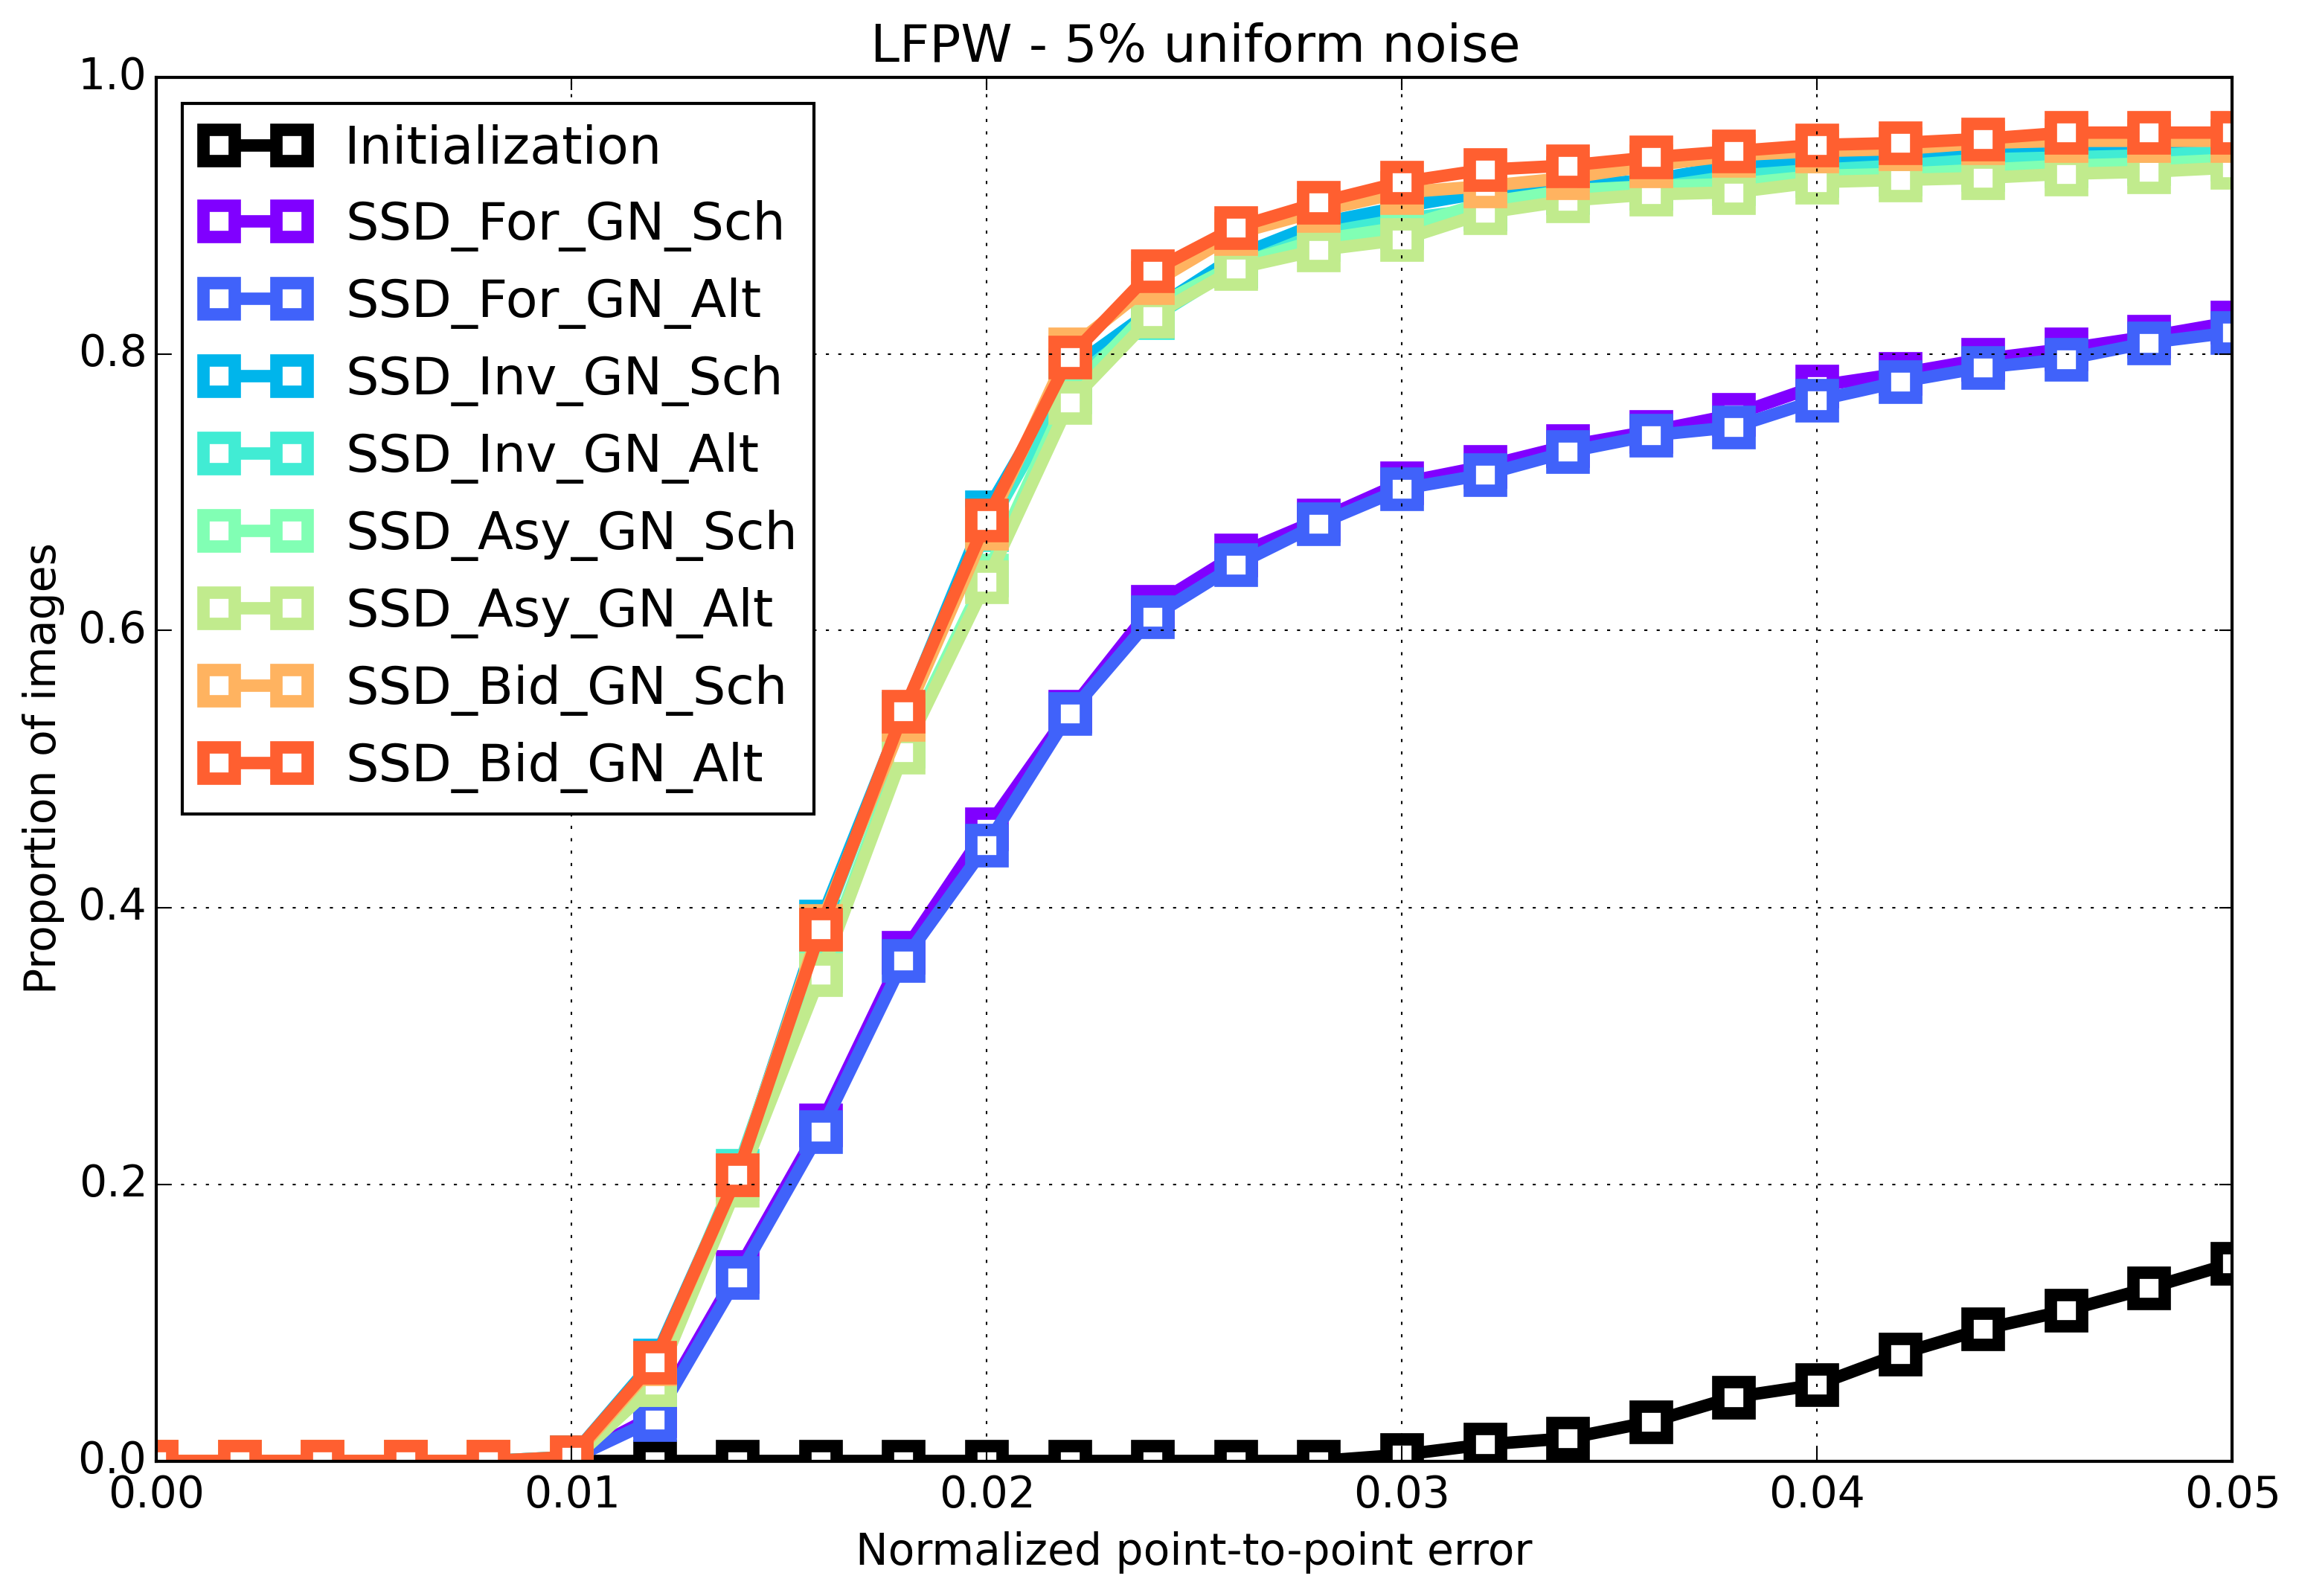
\includegraphics[width=\textwidth]{experiments/algorithms/ssd_gn/ced_ssd_gn_5.png}
	    \caption{Cumulative Error Distribution graph on the LFPW test dataset for all SSD Gauss-Newton algorithms initialized with $5\%$ uniform noise.}
	    \label{fig:ced_ssd_gn_5}
	\end{subfigure}
	\hfill
	\begin{subfigure}{0.48\textwidth}
	    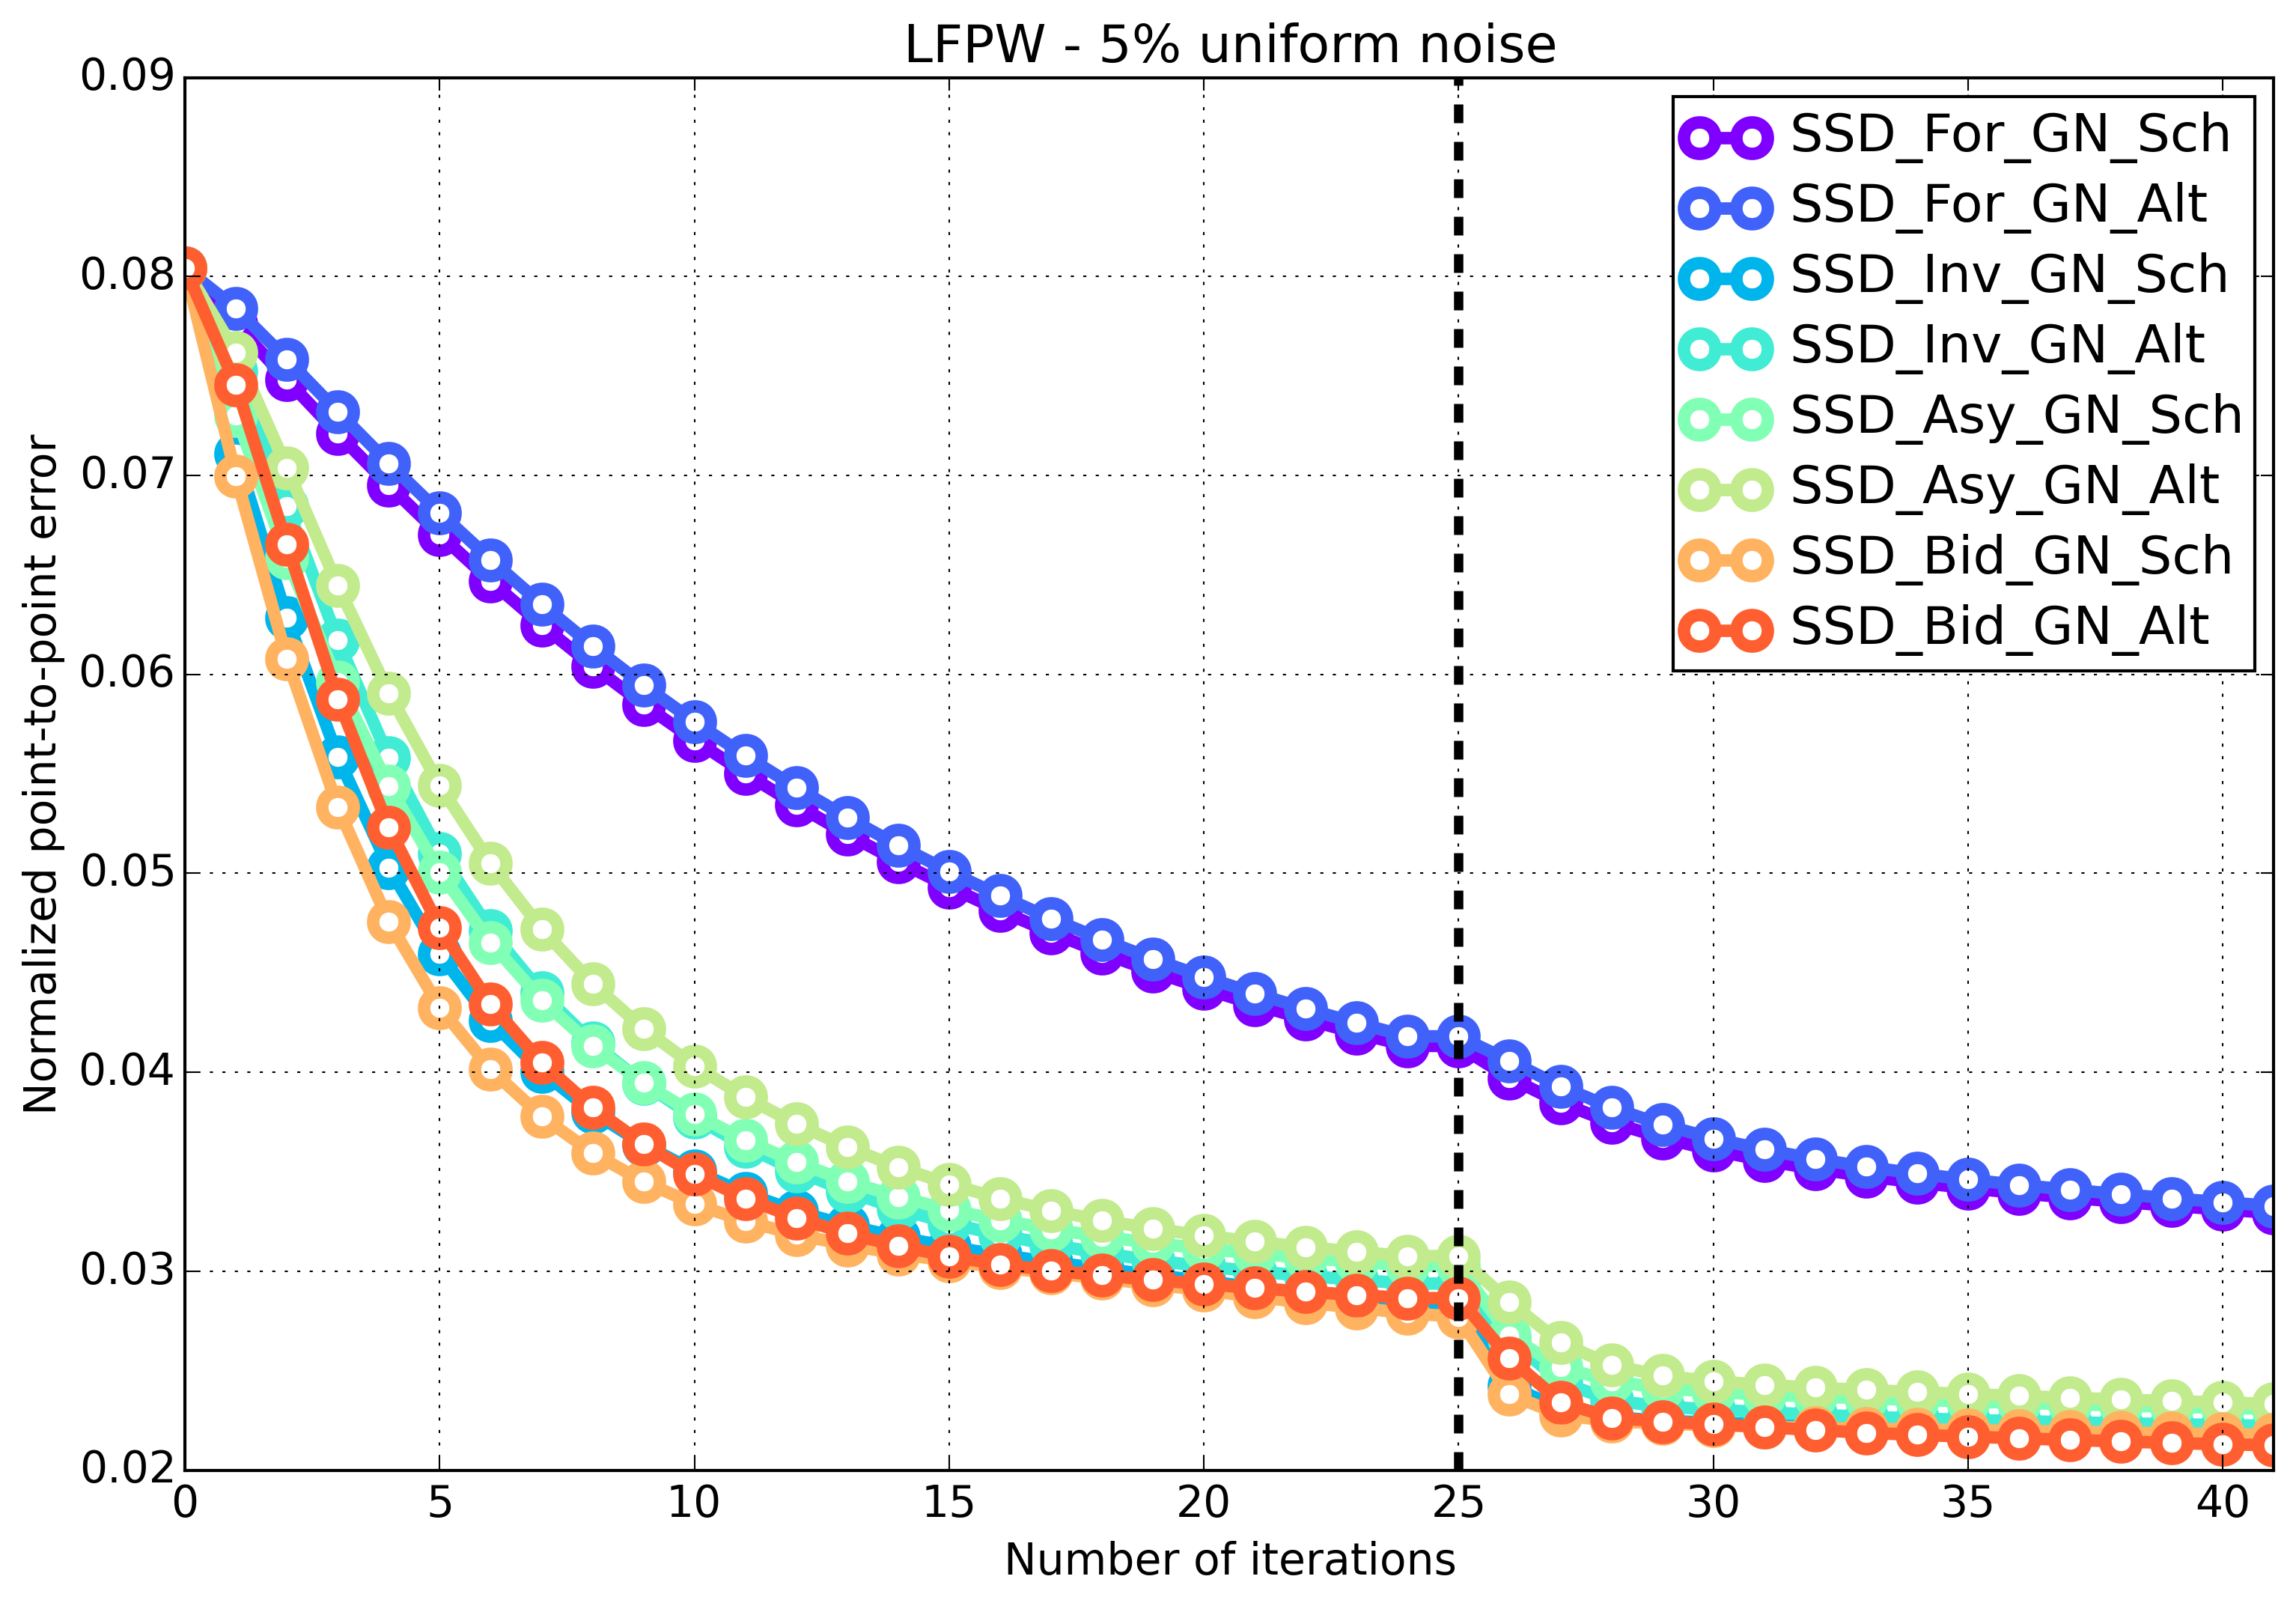
\includegraphics[width=\textwidth]{experiments/algorithms/ssd_gn/mean_error_vs_iters_ssd_gn_5.png}
	    \caption{Mean normalized point-to-point error vs number of iterations graph on the LFPW test dataset for all SSD Gauss-Newton algorithms initialized with $5\%$ uniform noise.}
	    \label{fig:mean_error_vs_iters_ssd_gn_5}
	\end{subfigure}
	\par\medskip
	\begin{subfigure}{0.48\textwidth}
	    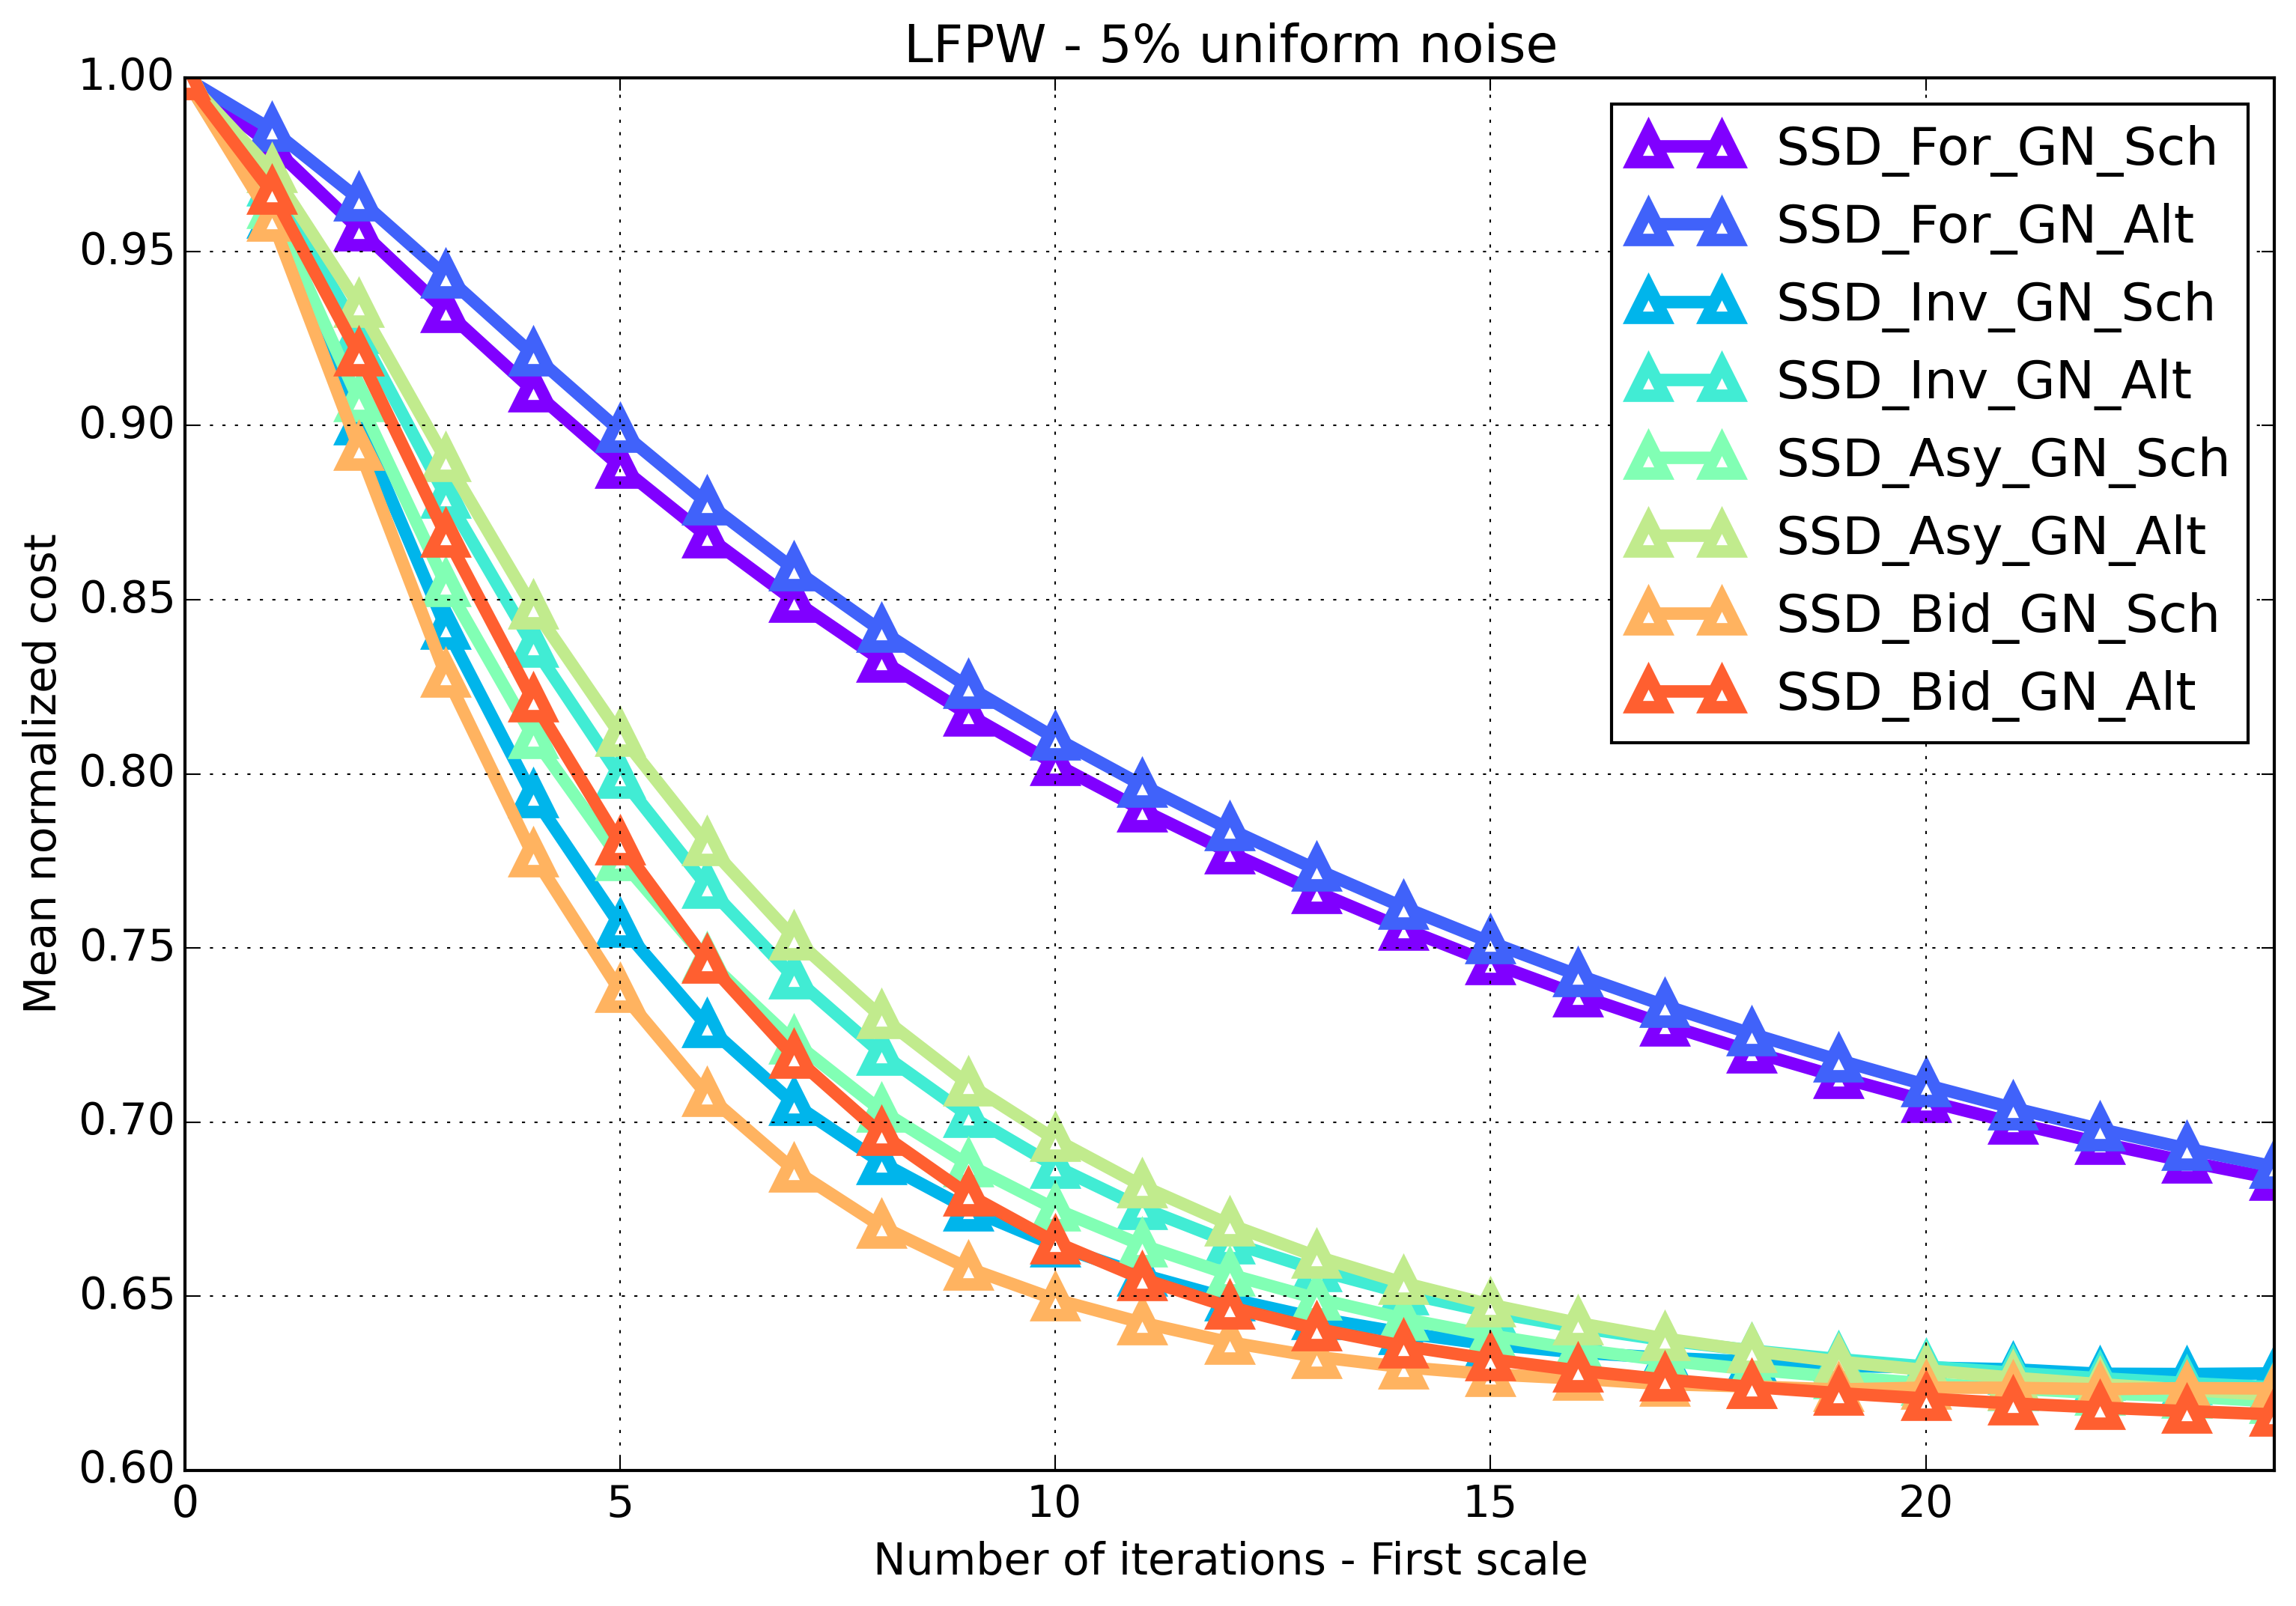
\includegraphics[width=\textwidth]{experiments/algorithms/ssd_gn/mean_cost_vs_iters1_ssd_gn_5.png}
	    \caption{Mean normalized cost vs number of first scale iterations graph on the LFPW test dataset for all SSD Gauss-Newton algorithms initialized with $5\%$ uniform noise.}
	    \label{fig:mean_cost_vs_iters1_ssd_gn_5}
	\end{subfigure}
	\hfill
	\begin{subfigure}{0.48\textwidth}
	    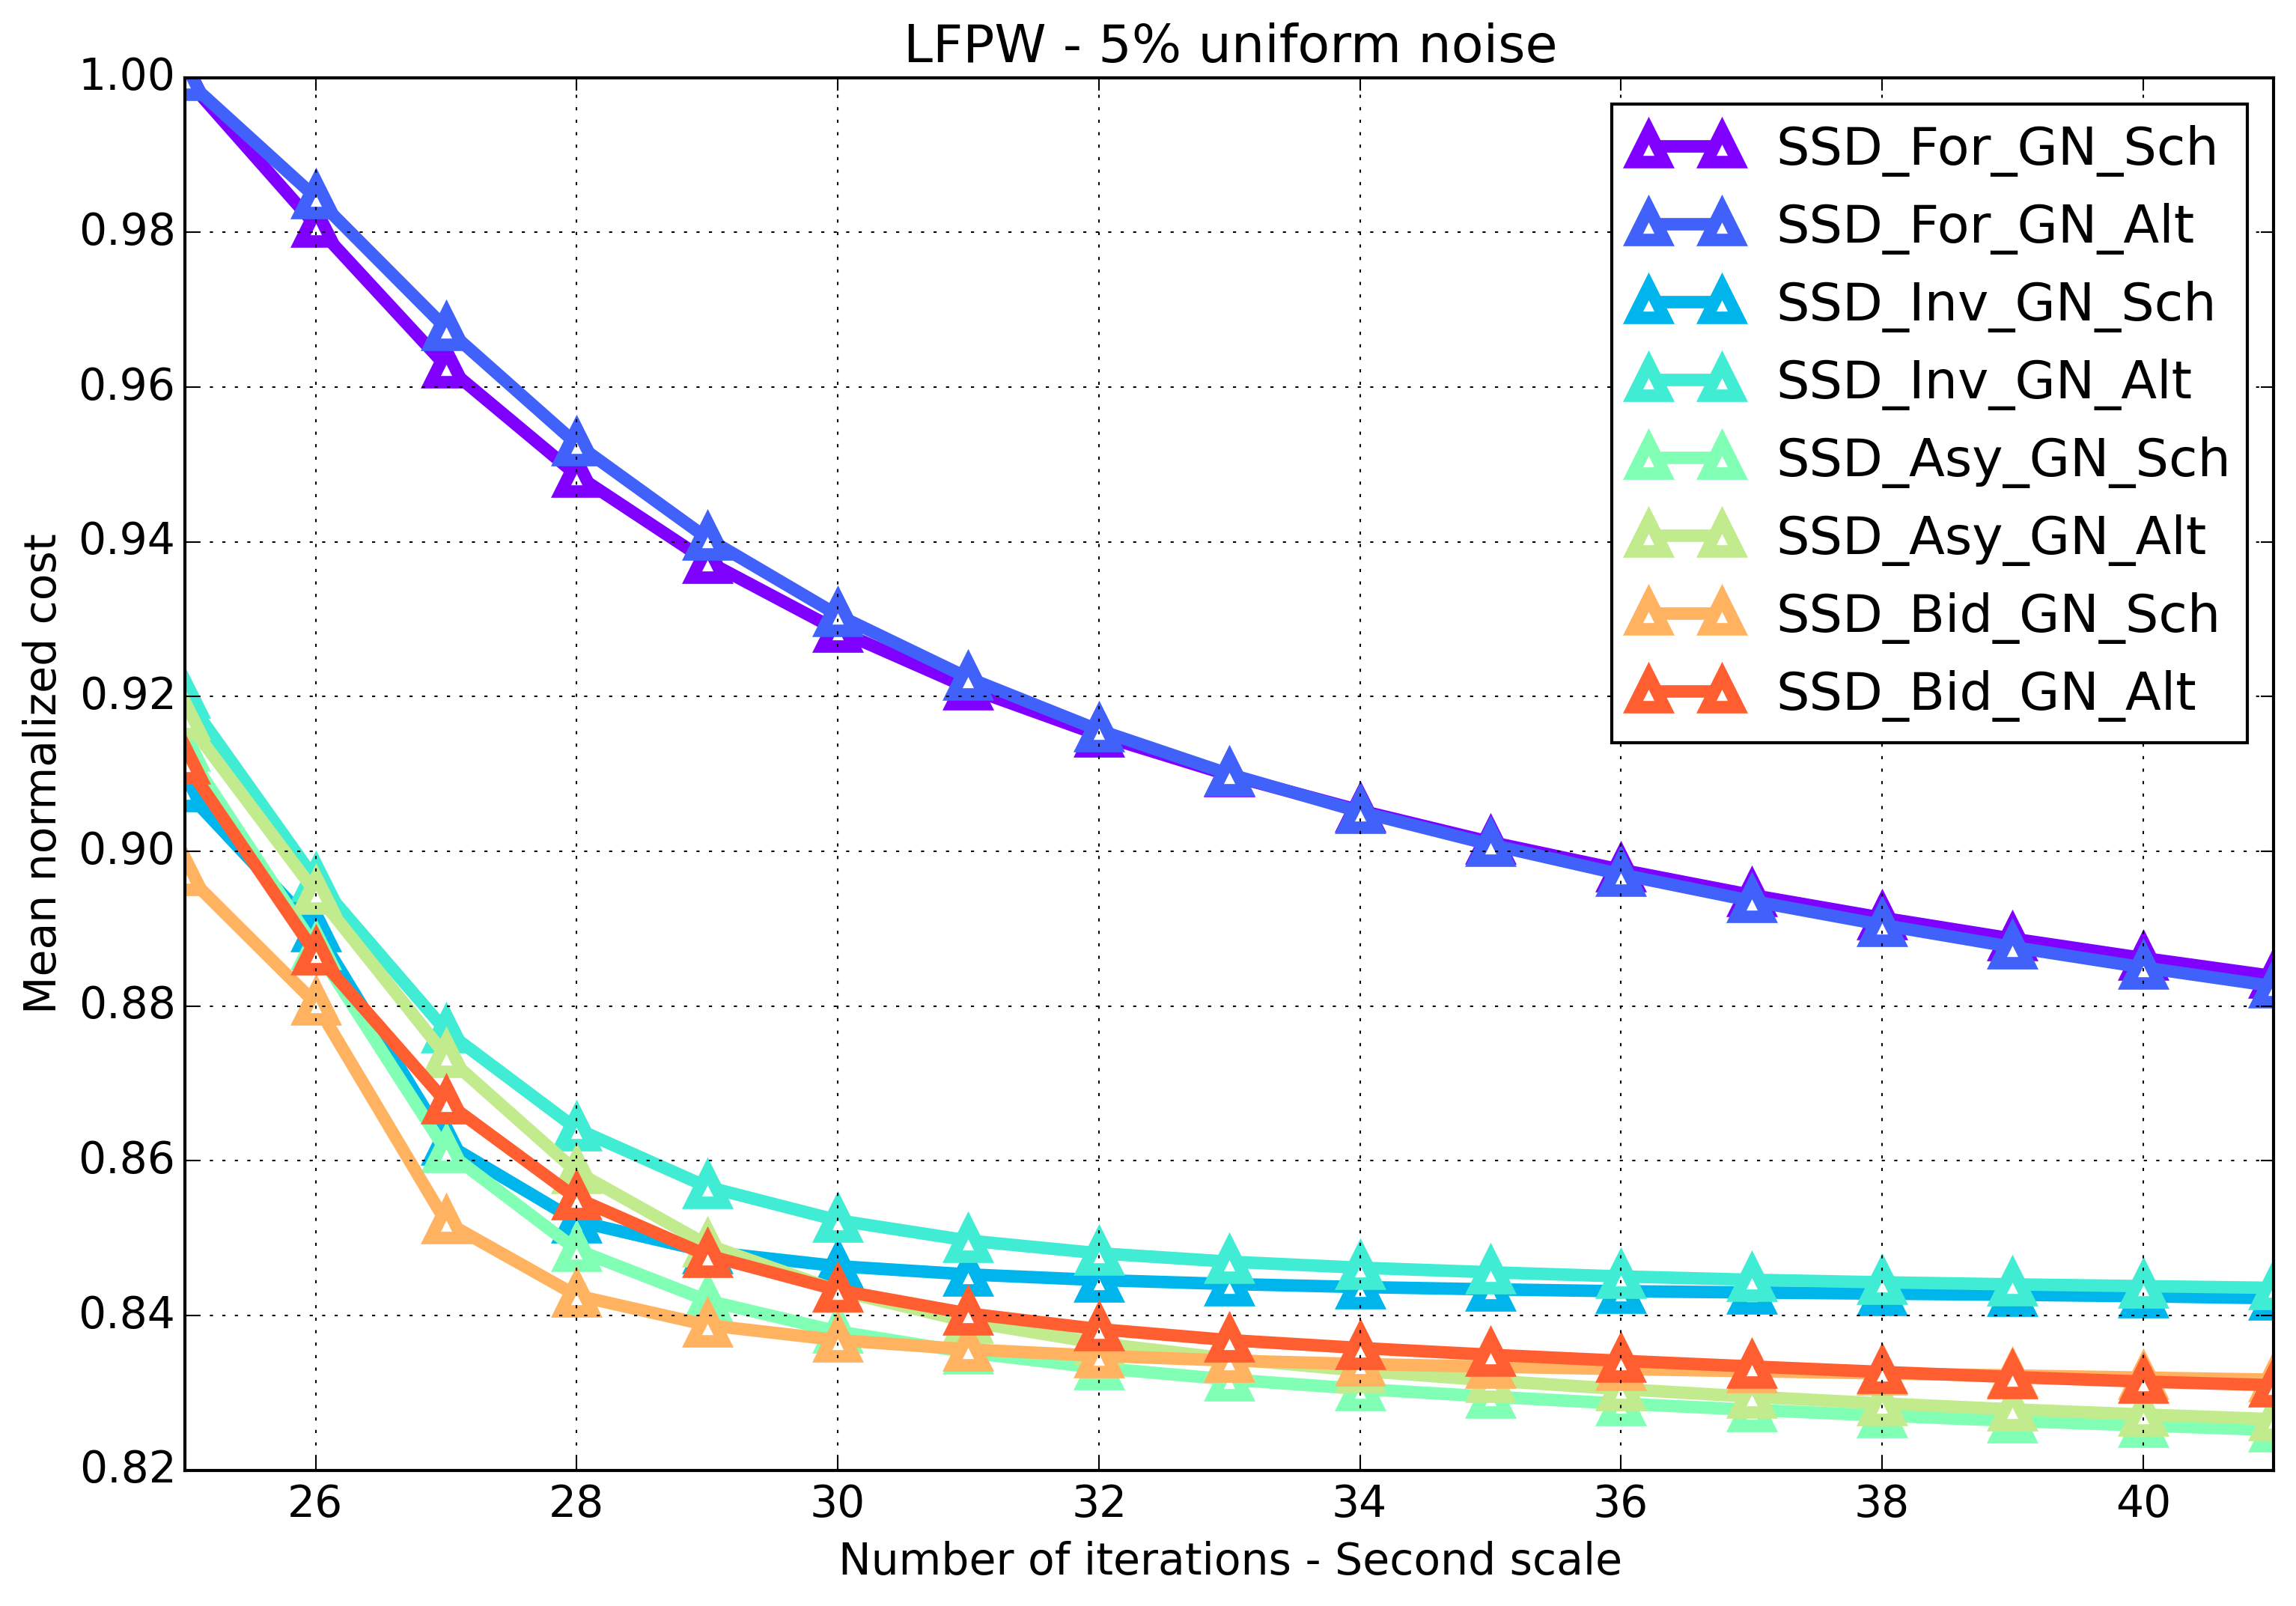
\includegraphics[width=\textwidth]{experiments/algorithms/ssd_gn/mean_cost_vs_iters2_ssd_gn_5.png}
	    \caption{Mean normalized cost vs number of second scale iterations graph on the LFPW test dataset for all SSD Gauss-Newton algorithms initialized with $5\%$ uniform noise.}
	    \label{fig:mean_cost_vs_iters2_ssd_gn_5}
	\end{subfigure}
	\label{fig:ssd_gn_5}
	\caption{}
\end{figure*}


\subsubsection*{Wiberg}

\begin{figure*}[h!]
	\centering
	\begin{subfigure}{0.48\textwidth}
	    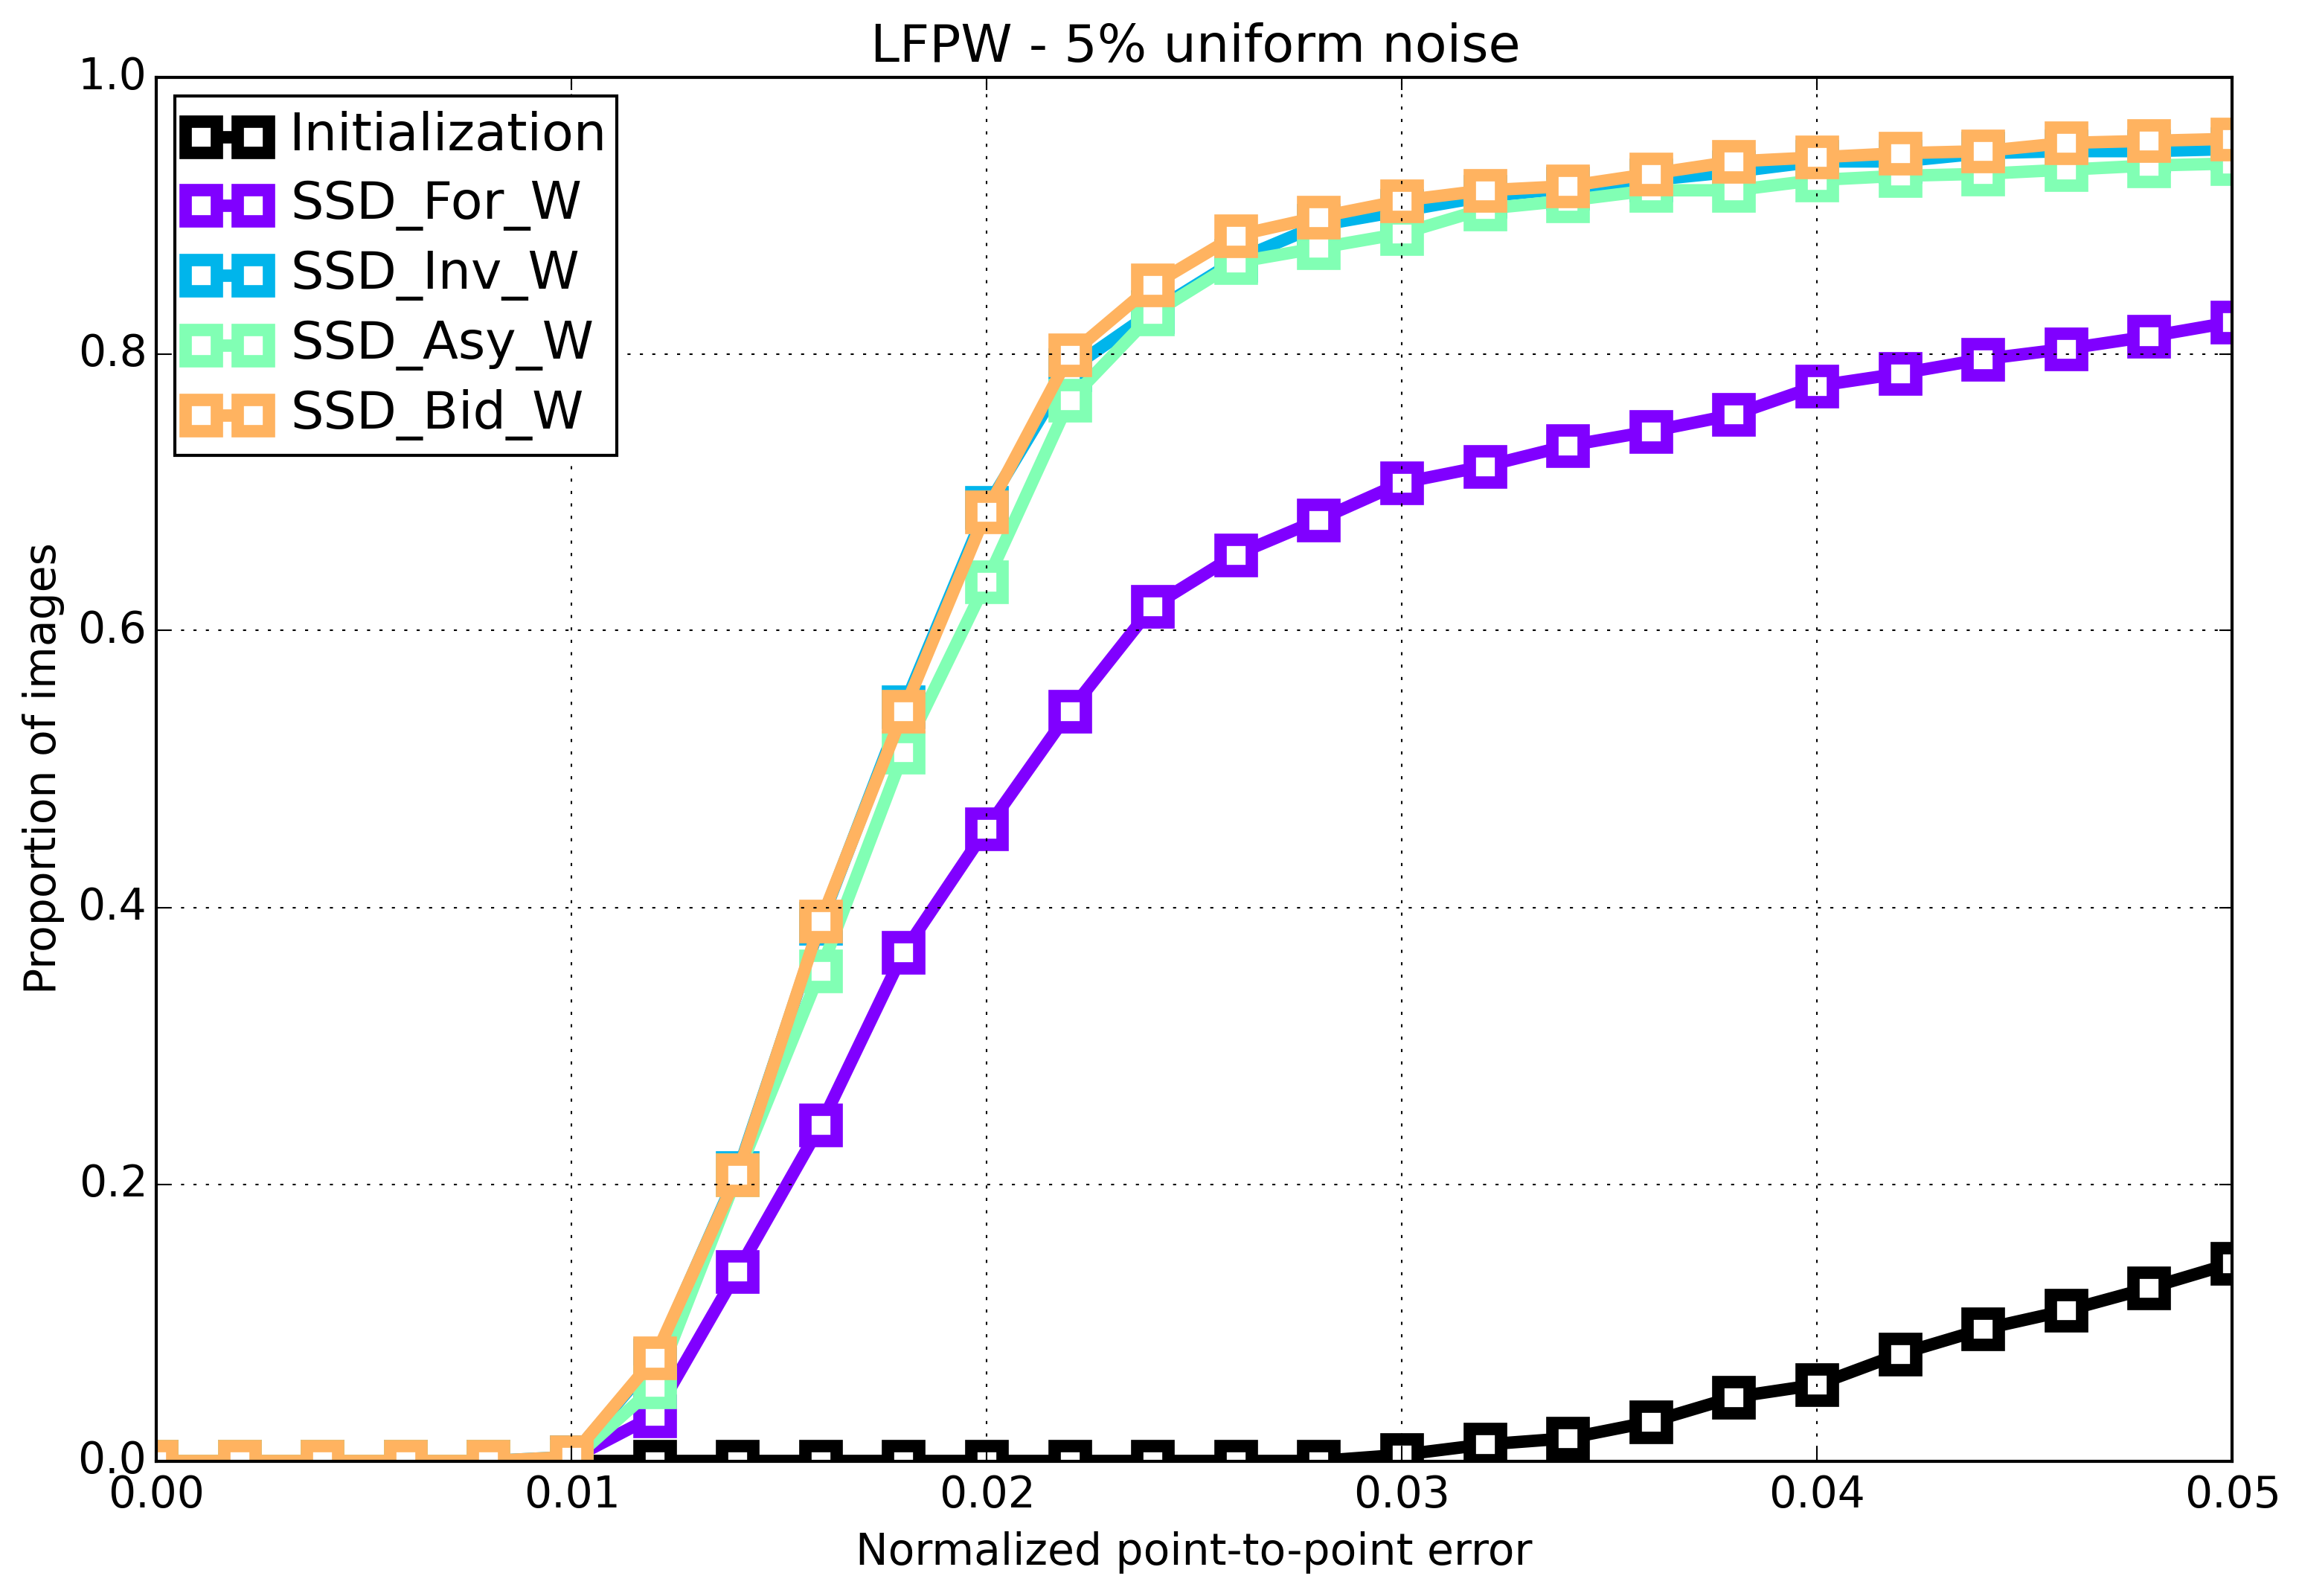
\includegraphics[width=\textwidth]{experiments/algorithms/ssd_w/ced_ssd_w_5.png}
	    \caption{Cumulative Error Distribution graph on the LFPW test dataset for all SSD Wiberg algorithms initialized with $5\%$ uniform noise.}
	    \label{fig:ced_ssd_w_5}
	\end{subfigure}
	\hfill
	\begin{subfigure}{0.48\textwidth}
	    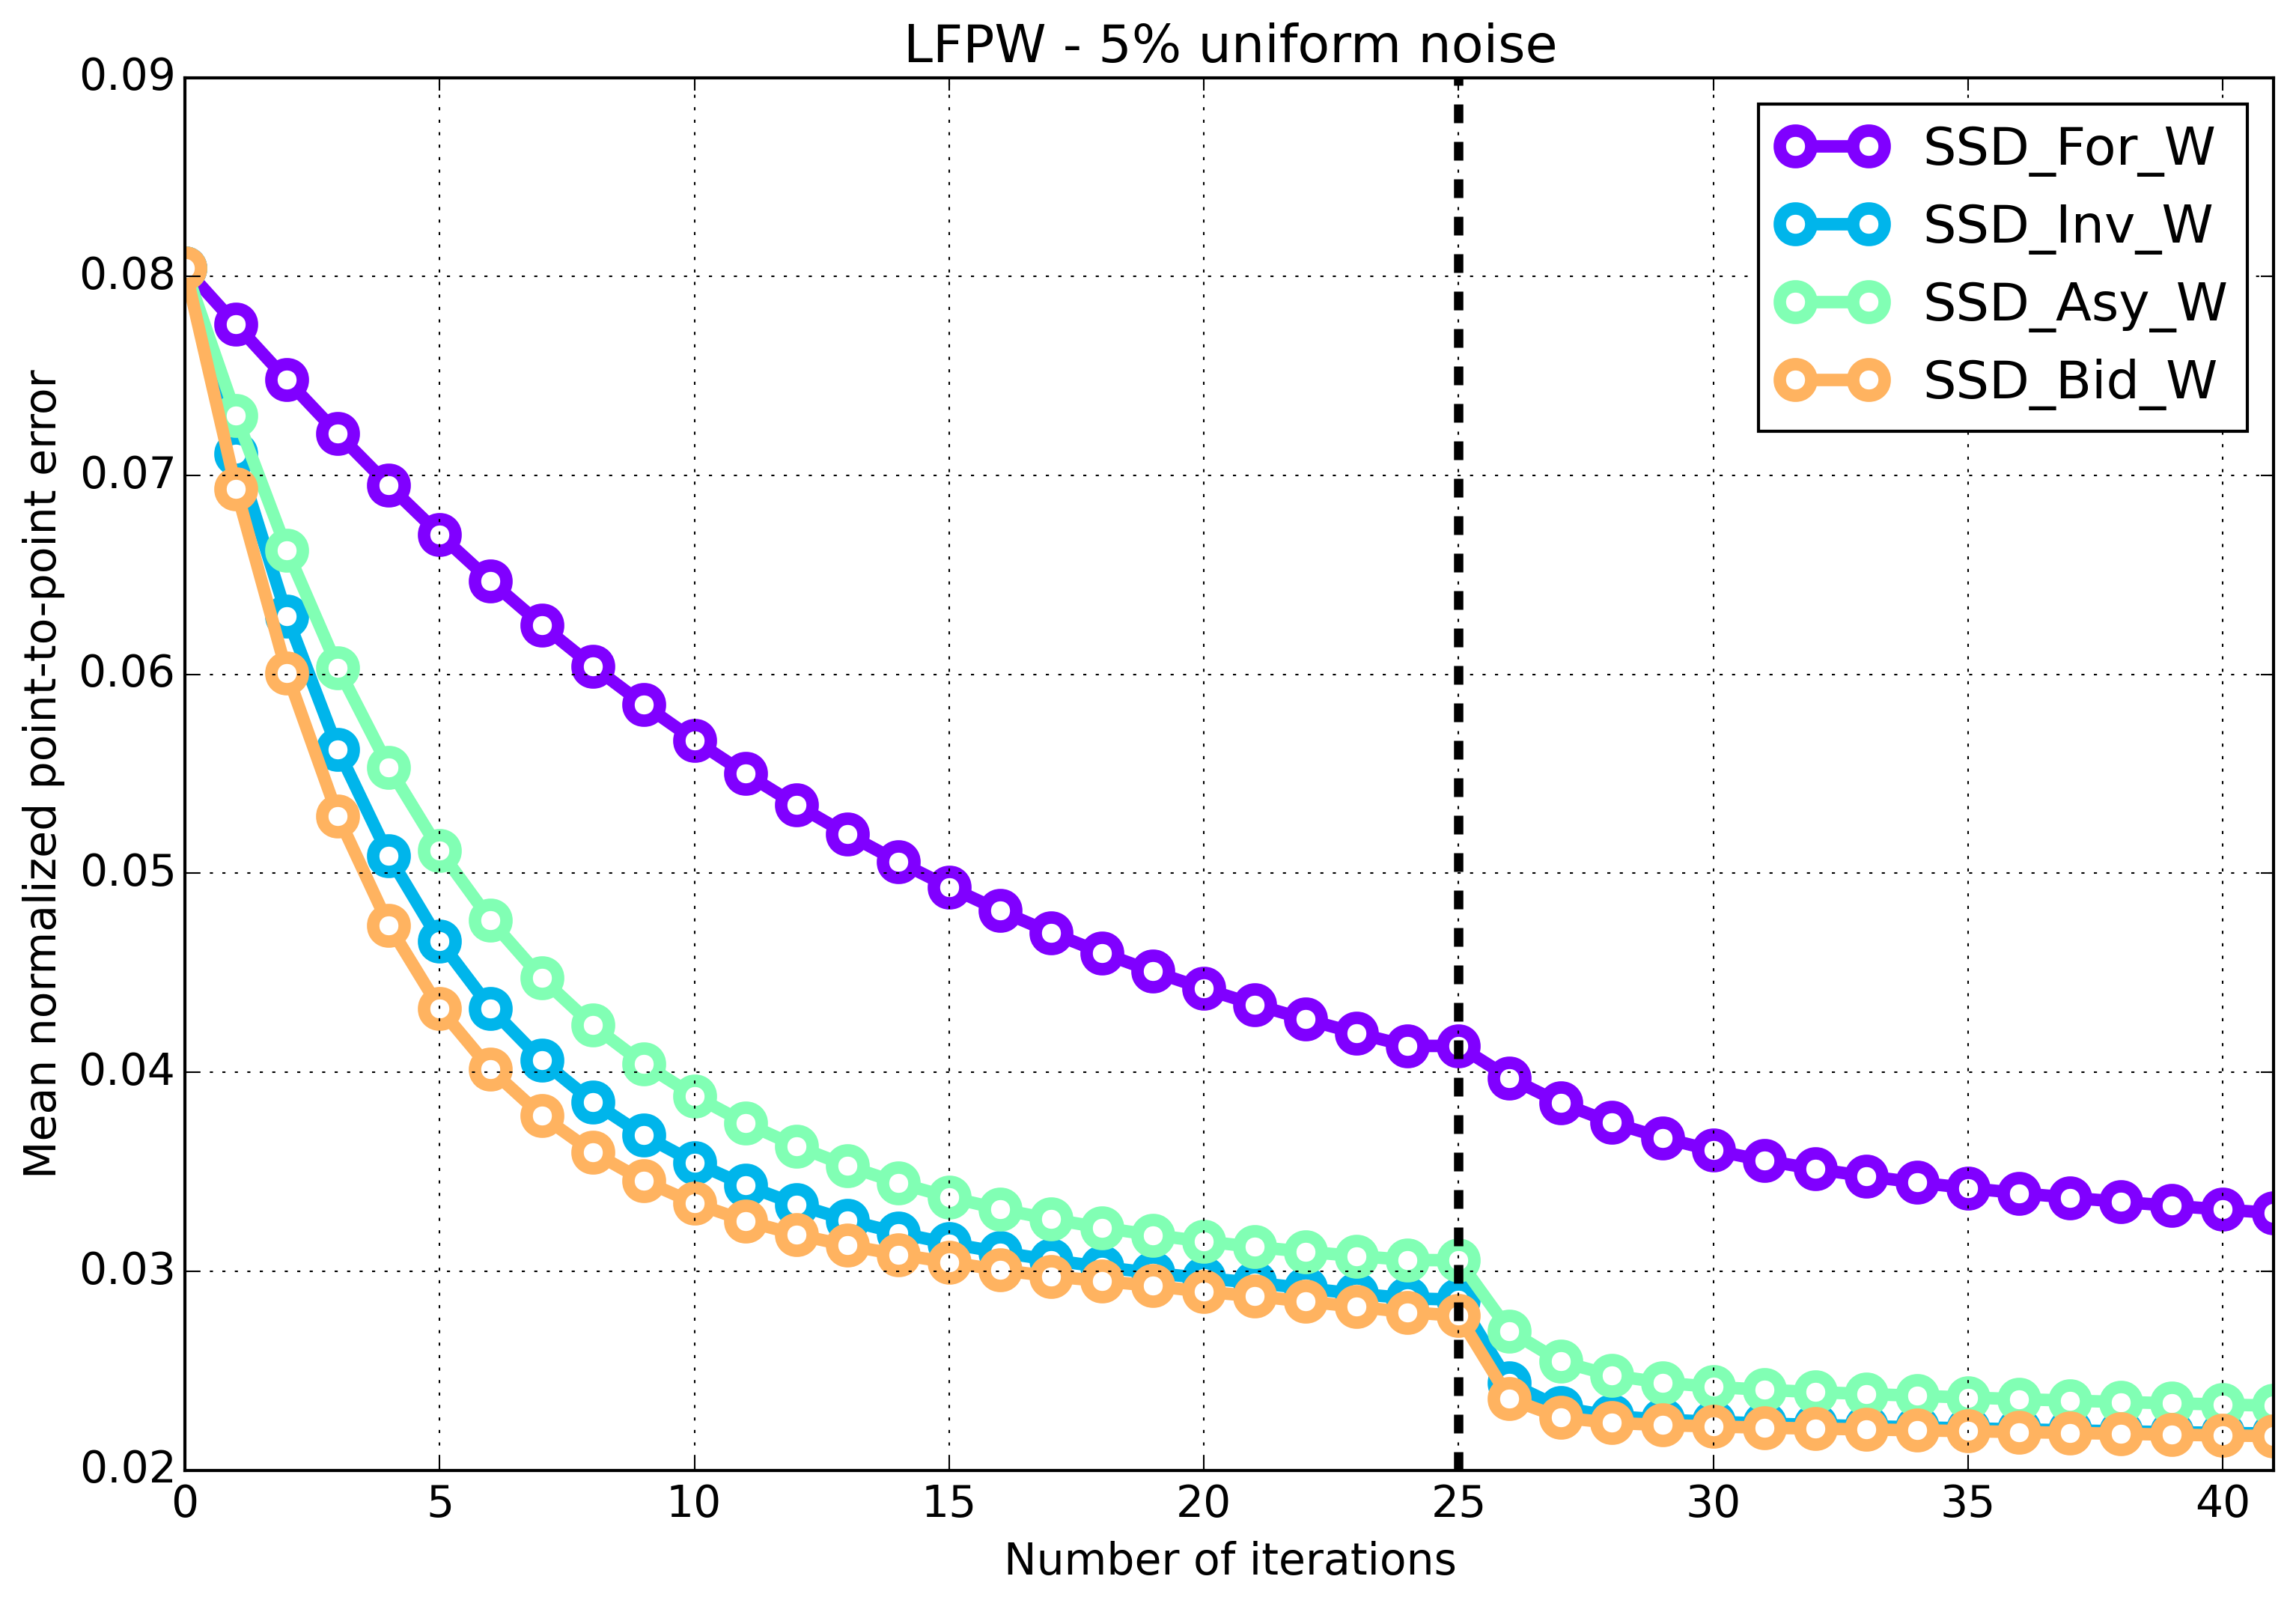
\includegraphics[width=\textwidth]{experiments/algorithms/ssd_w/mean_error_vs_iters_ssd_w_5.png}
	    \caption{Mean normalized point-to-point error vs number of iterations graph on the LFPW test dataset for all SSD Wiberg algorithms initialized with $5\%$ uniform noise.}
	    \label{fig:mean_error_vs_iters_ssd_w_5}
	\end{subfigure}
	\par\medskip
	\begin{subfigure}{0.48\textwidth}
	    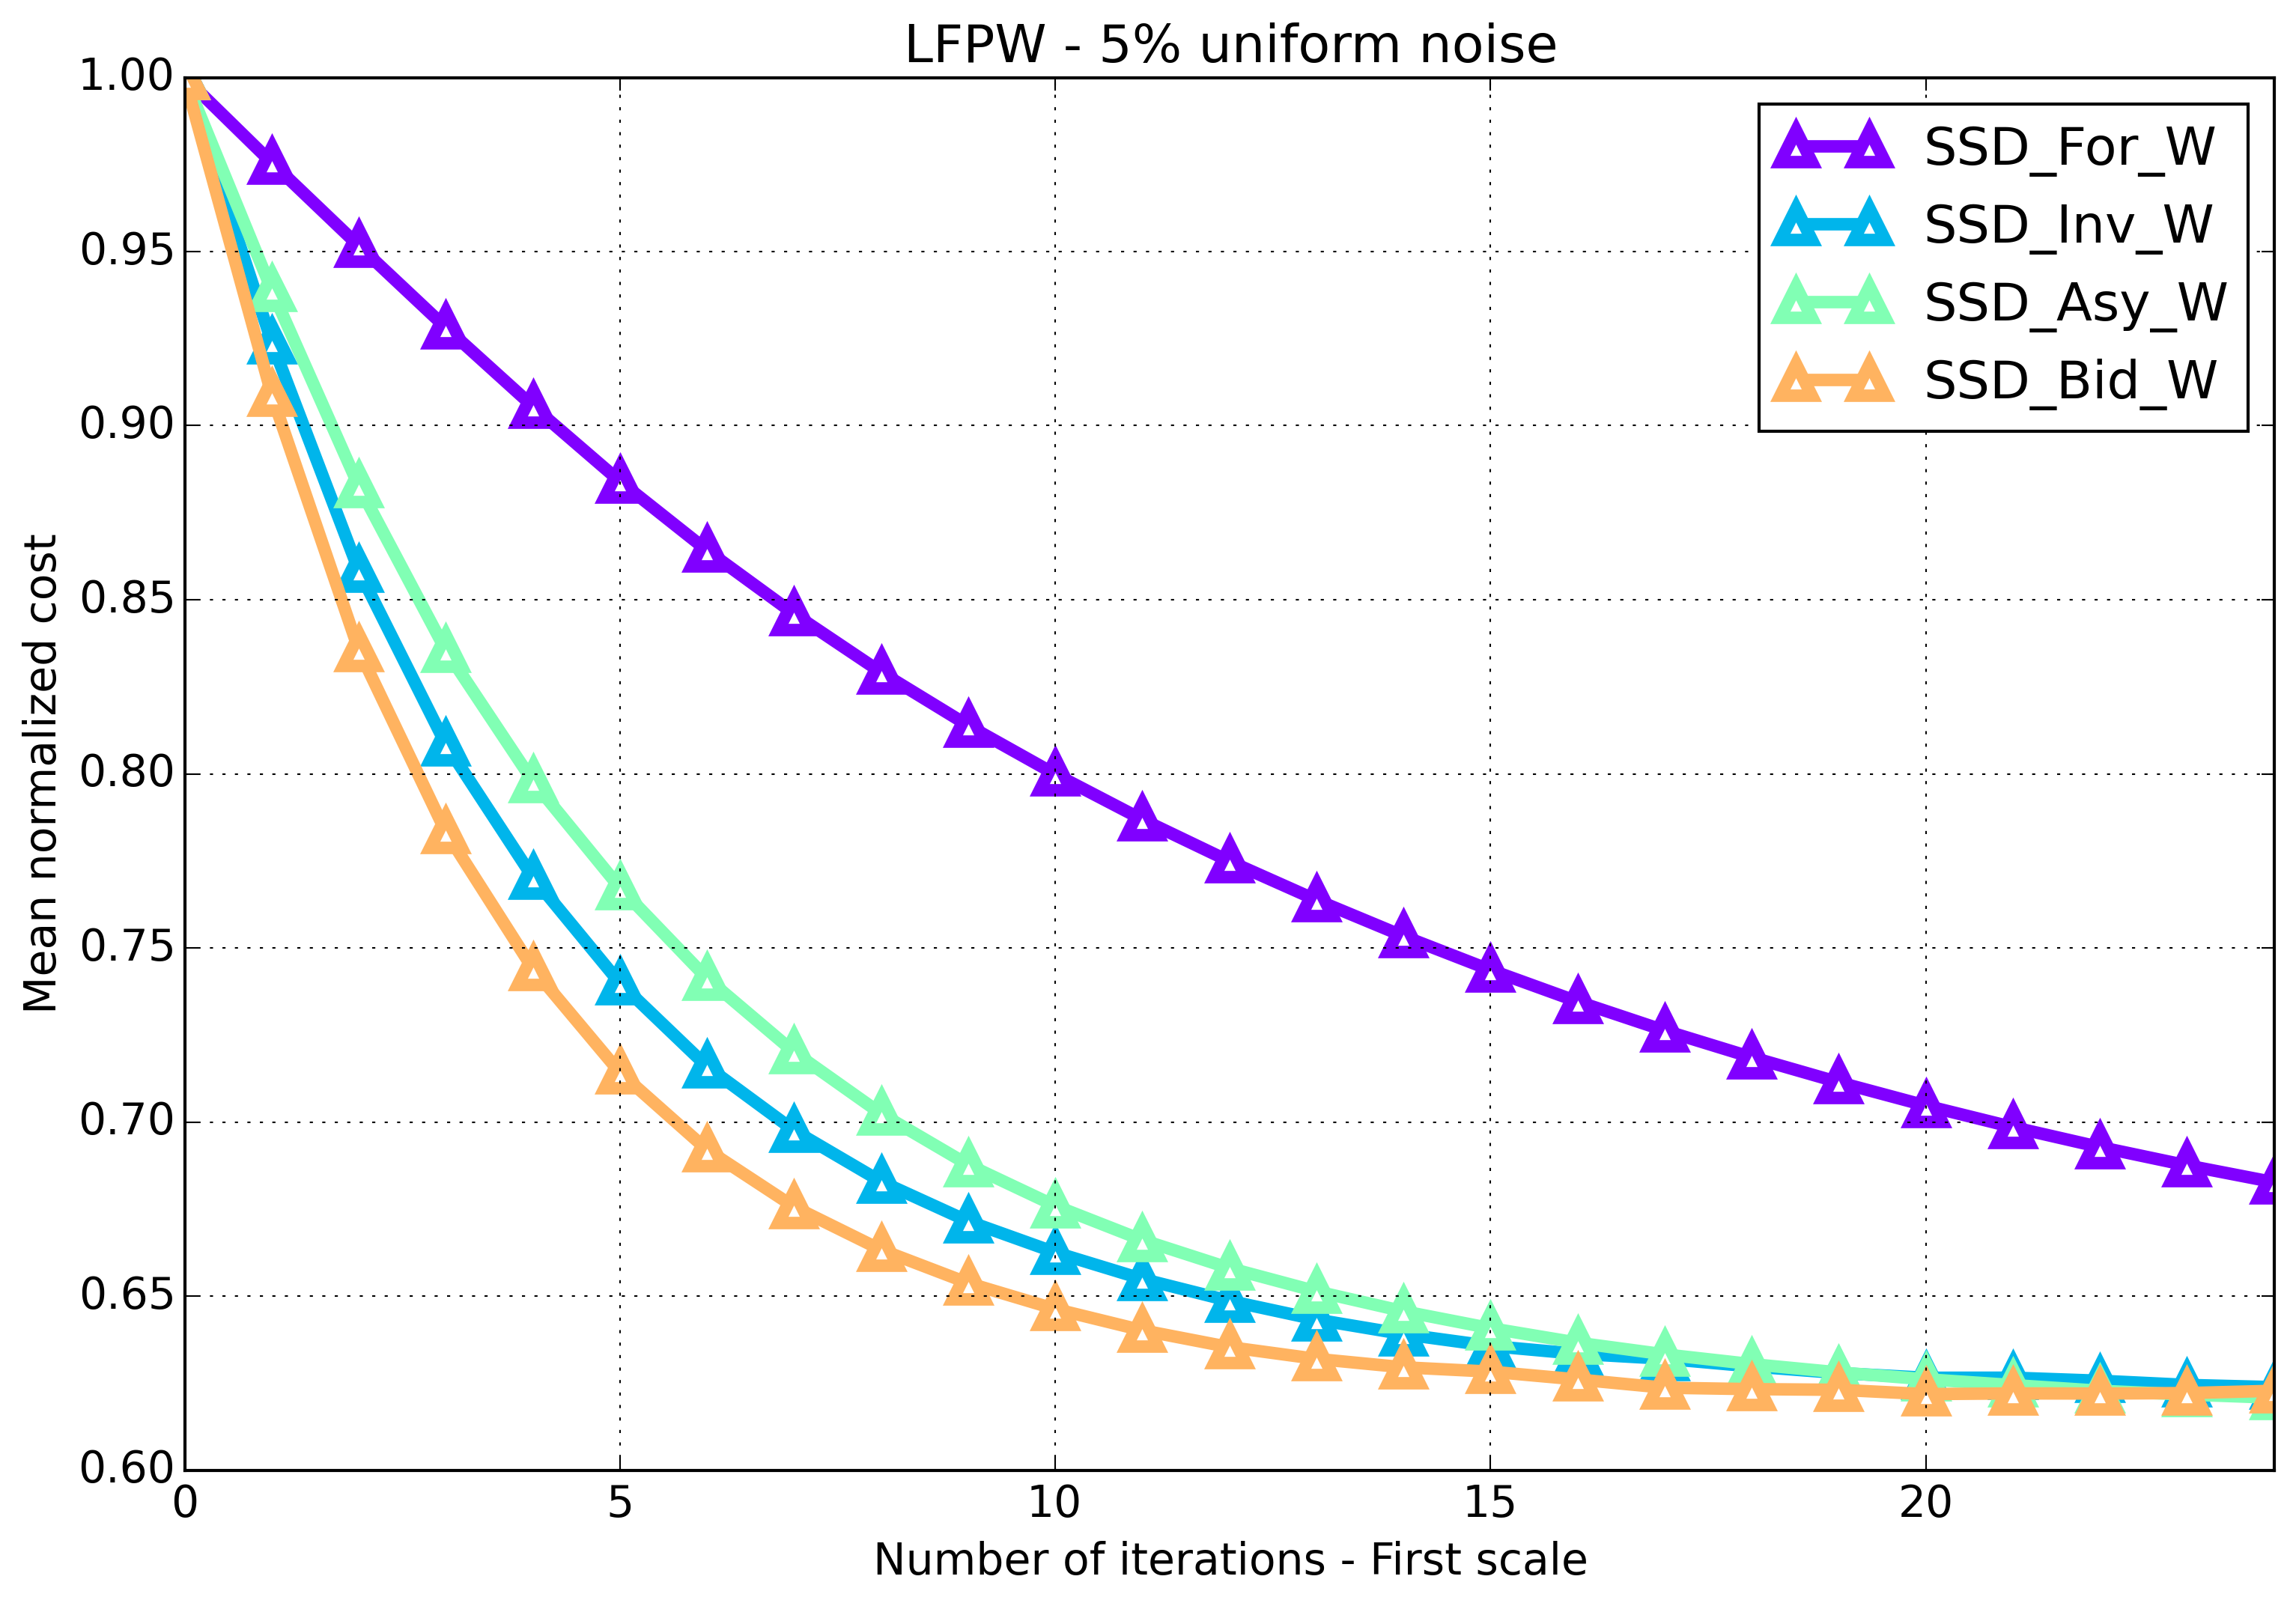
\includegraphics[width=\textwidth]{experiments/algorithms/ssd_w/mean_cost_vs_iters1_ssd_w_5.png}
	    \caption{Mean normalized cost vs number of first scale iterations graph on the LFPW test dataset for all SSD Wiberg algorithms initialized with $5\%$ uniform noise.}
	    \label{fig:mean_cost_vs_iters1_ssd_w_5}
	\end{subfigure}
	\hfill
	\begin{subfigure}{0.48\textwidth}
	    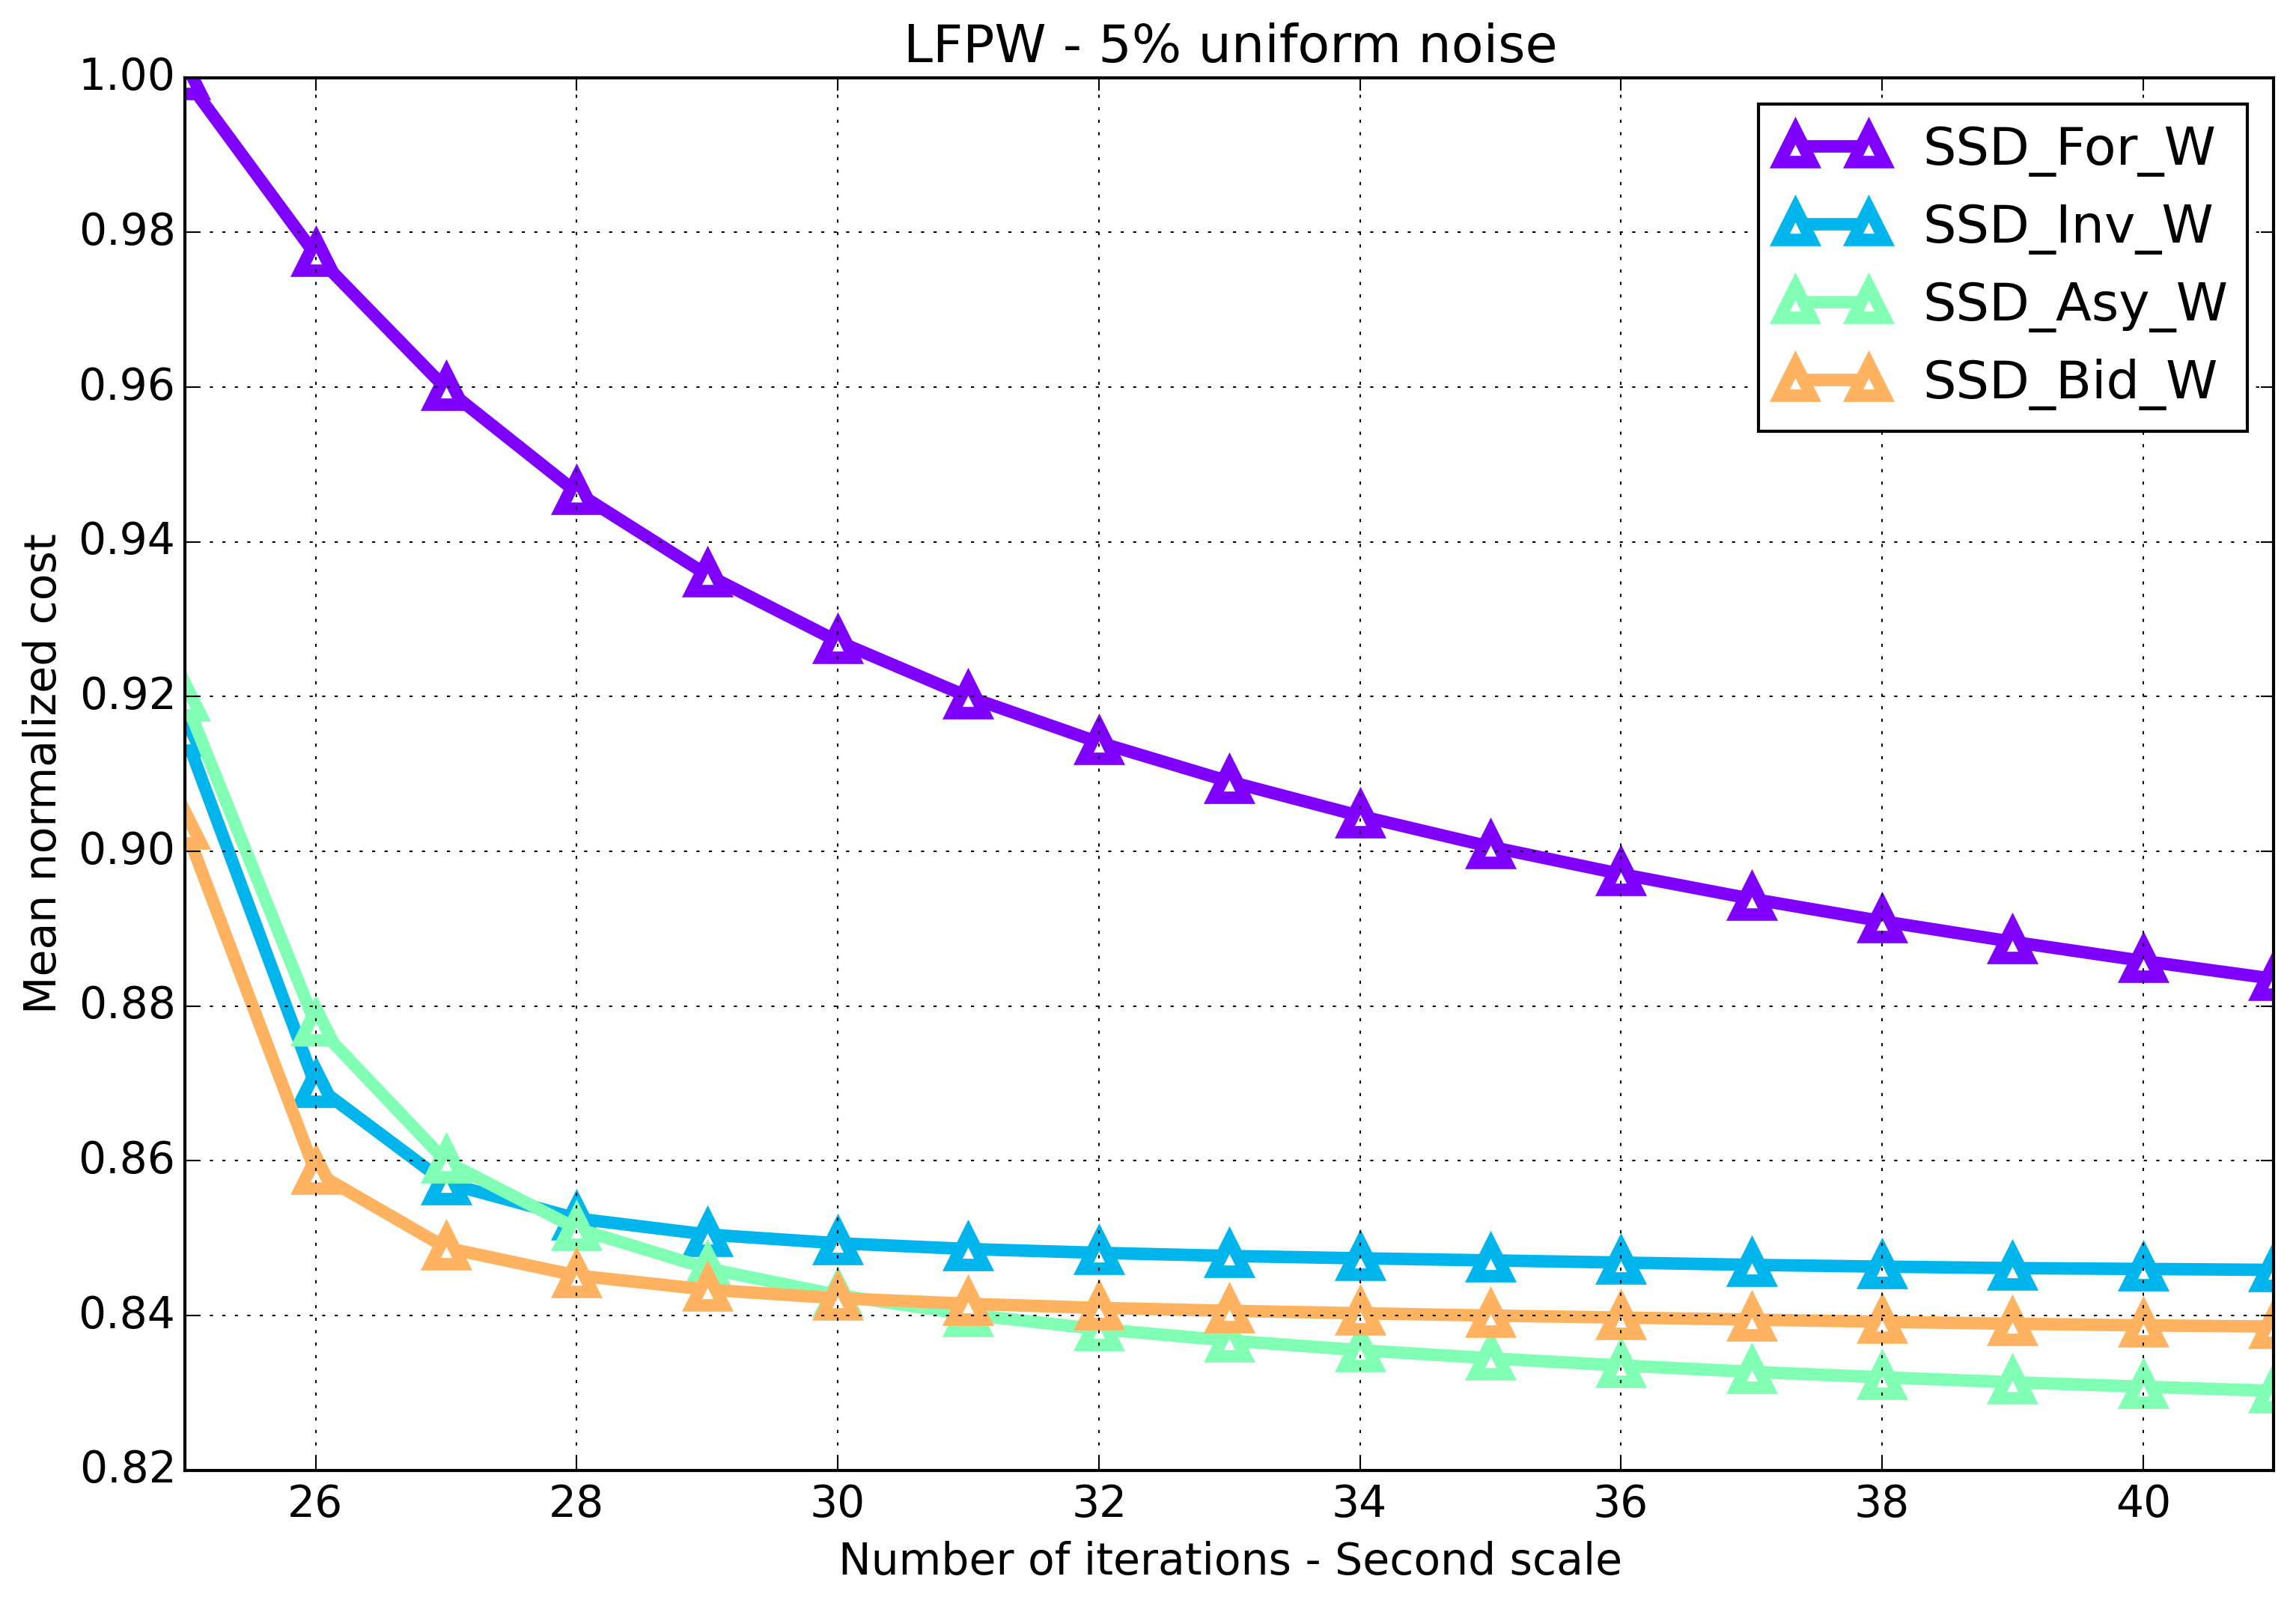
\includegraphics[width=\textwidth]{experiments/algorithms/ssd_w/mean_cost_vs_iters2_ssd_w_5.png}
	    \caption{Mean normalized cost vs number of second scale iterations graph on the LFPW test dataset for all SSD Wiberg algorithms initialized with $5\%$ uniform noise.}
	    \label{fig:mean_cost_vs_iters2_ssd_w_5}
	\end{subfigure}
	\label{fig:ssd_w_5}
	\caption{}
\end{figure*}


\subsubsection{Project-Out algorithms}


\subsubsection*{Gauss-Newton}

\begin{figure*}[h!]
	\centering
	\begin{subfigure}{0.48\textwidth}
	    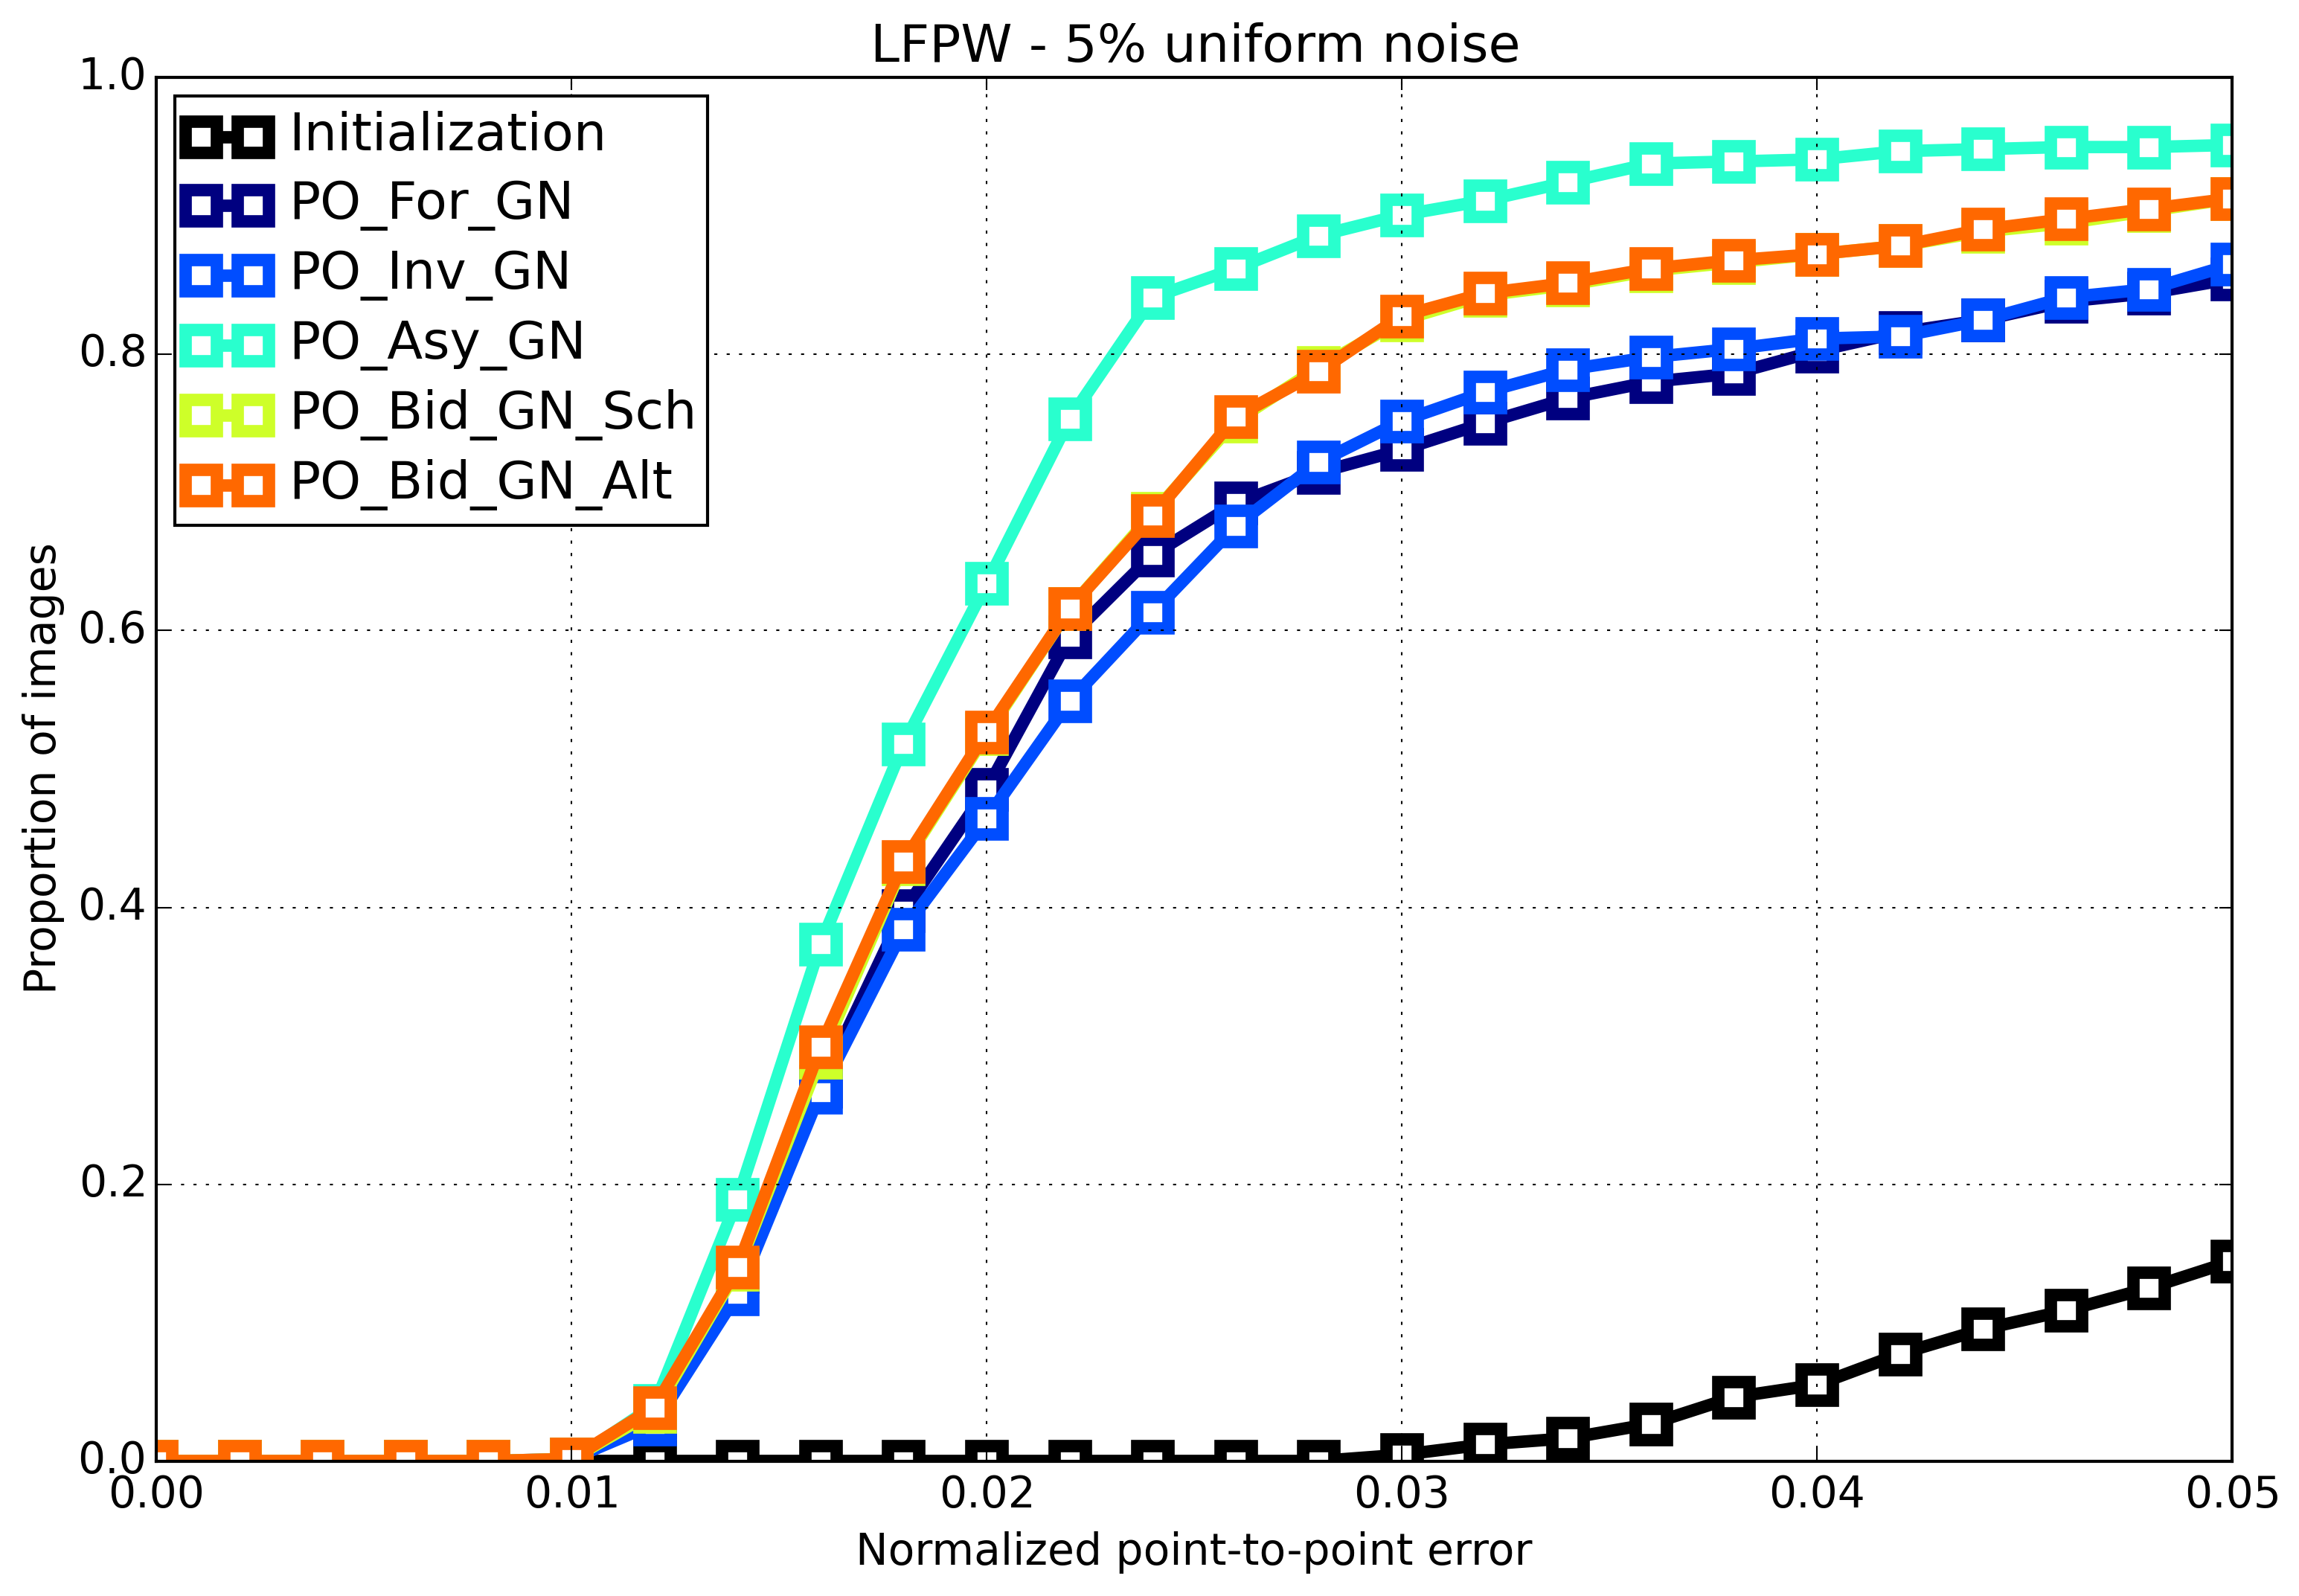
\includegraphics[width=\textwidth]{experiments/algorithms/po_gn/ced_po_gn_5.png}
	    \caption{Cumulative Error Distribution graph on the LFPW test dataset for all Project-Out Gauss-Newton algorithms initialized with $5\%$ uniform noise.}
	    \label{fig:ced_po_gn_5}
	\end{subfigure}
	\hfill
	\begin{subfigure}{0.48\textwidth}
	    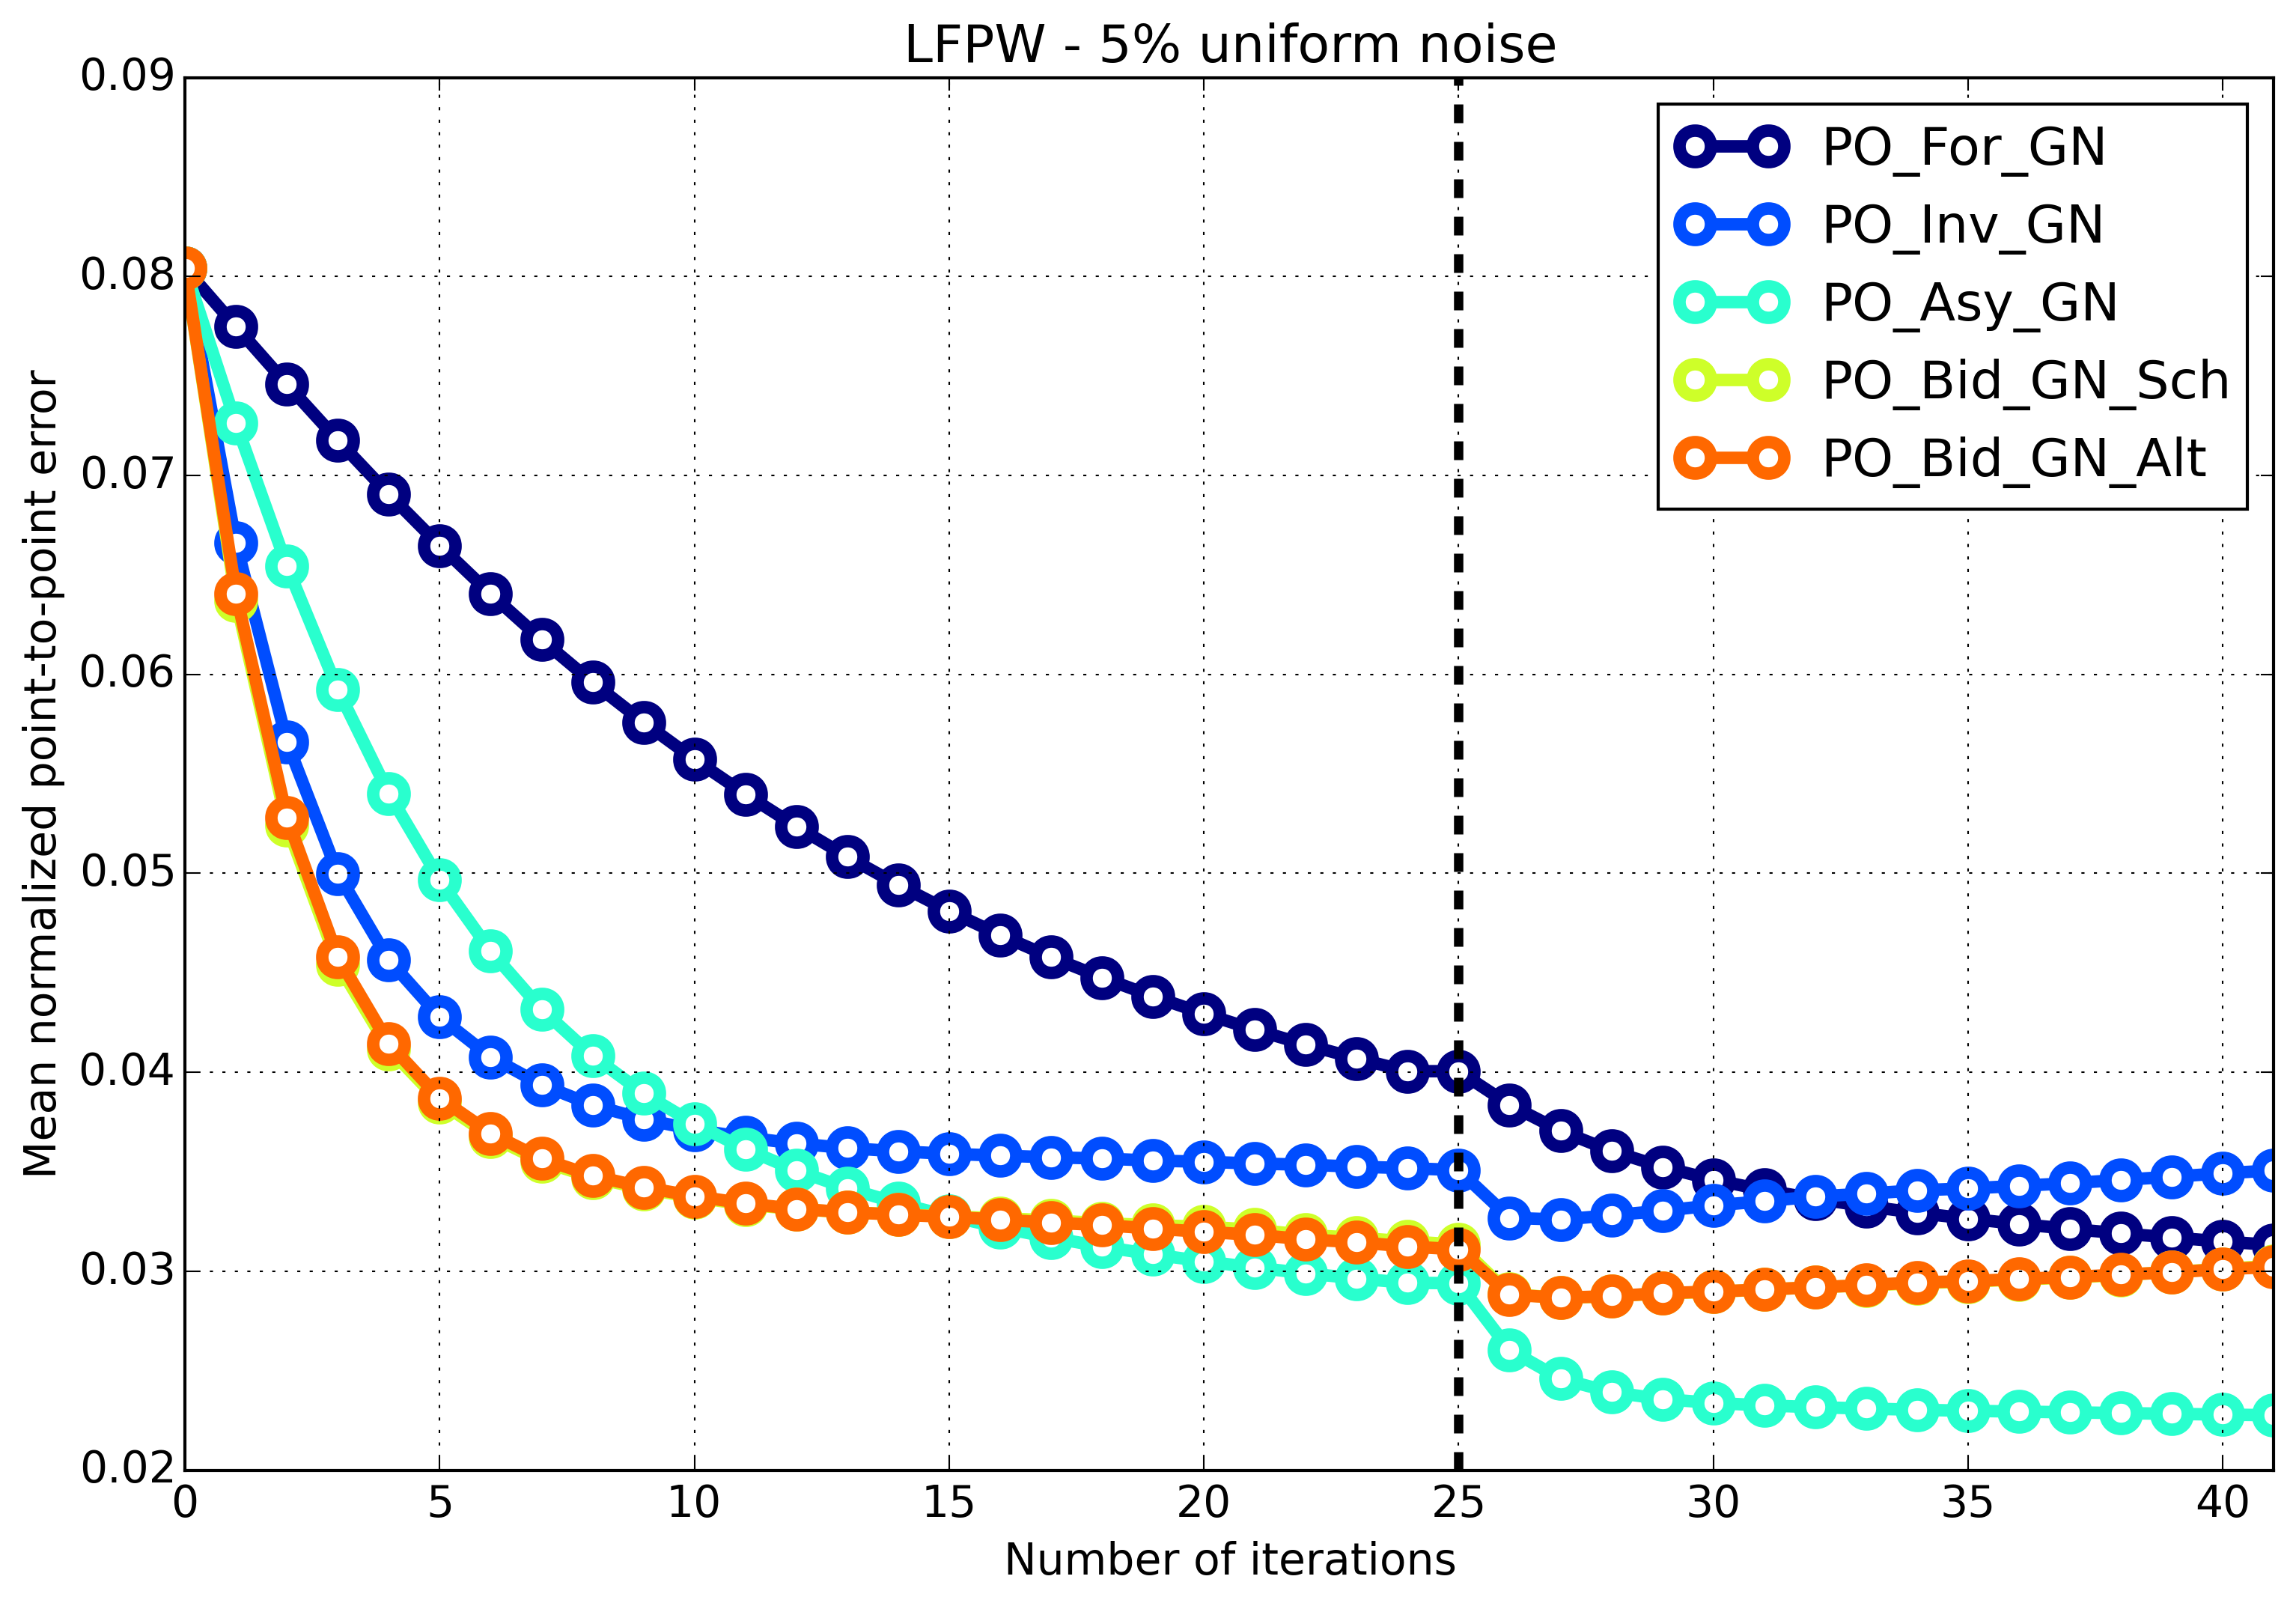
\includegraphics[width=\textwidth]{experiments/algorithms/po_gn/mean_error_vs_iters_po_gn_5.png}
	    \caption{Mean normalized point-to-point error vs number of iterations graph on the LFPW test dataset for all Project-Out Gauss-Newton algorithms initialized with $5\%$ uniform noise.}
	    \label{fig:mean_error_vs_iters_po_gn_5}
	\end{subfigure}
	\par\medskip
	\begin{subfigure}{0.48\textwidth}
	    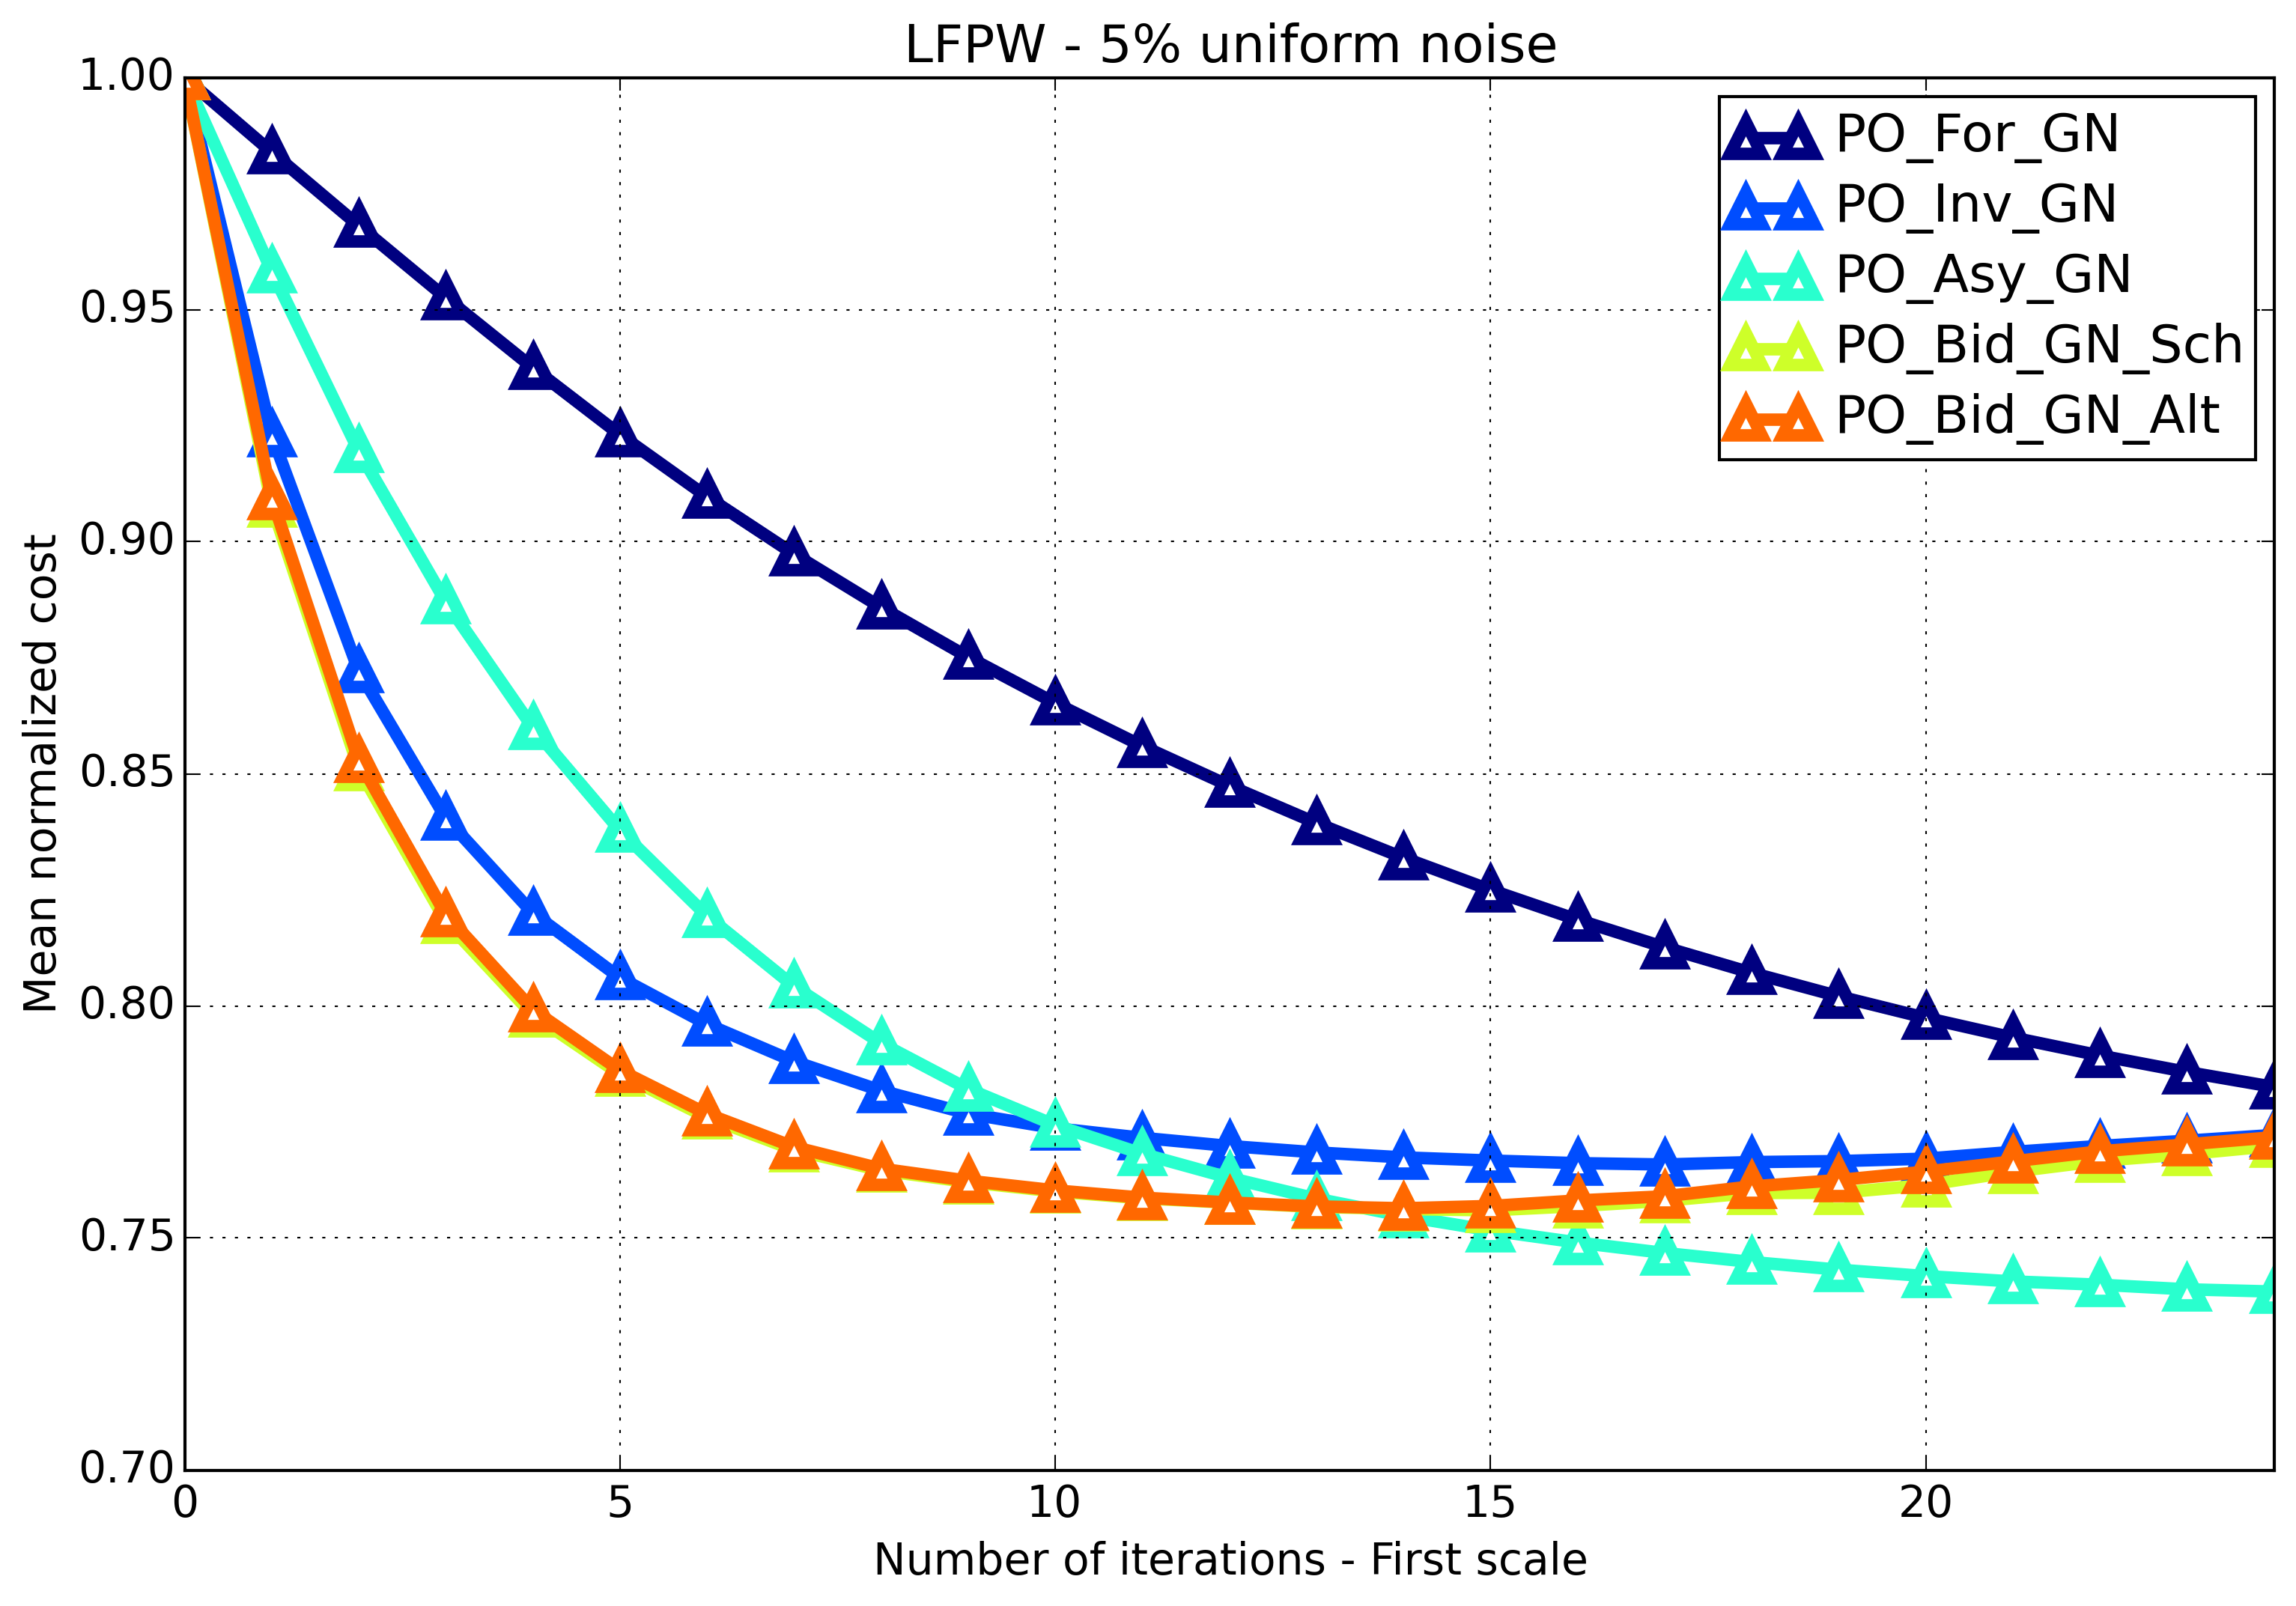
\includegraphics[width=\textwidth]{experiments/algorithms/po_gn/mean_cost_vs_iters1_po_gn_5.png}
	    \caption{Mean normalized cost vs number of first scale iterations graph on the LFPW test dataset for all Project-Out Gauss-Newton algorithms initialized with $5\%$ uniform noise.}
	    \label{fig:mean_cost_vs_iters1_po_gn_5}
	\end{subfigure}
	\hfill
	\begin{subfigure}{0.48\textwidth}
	    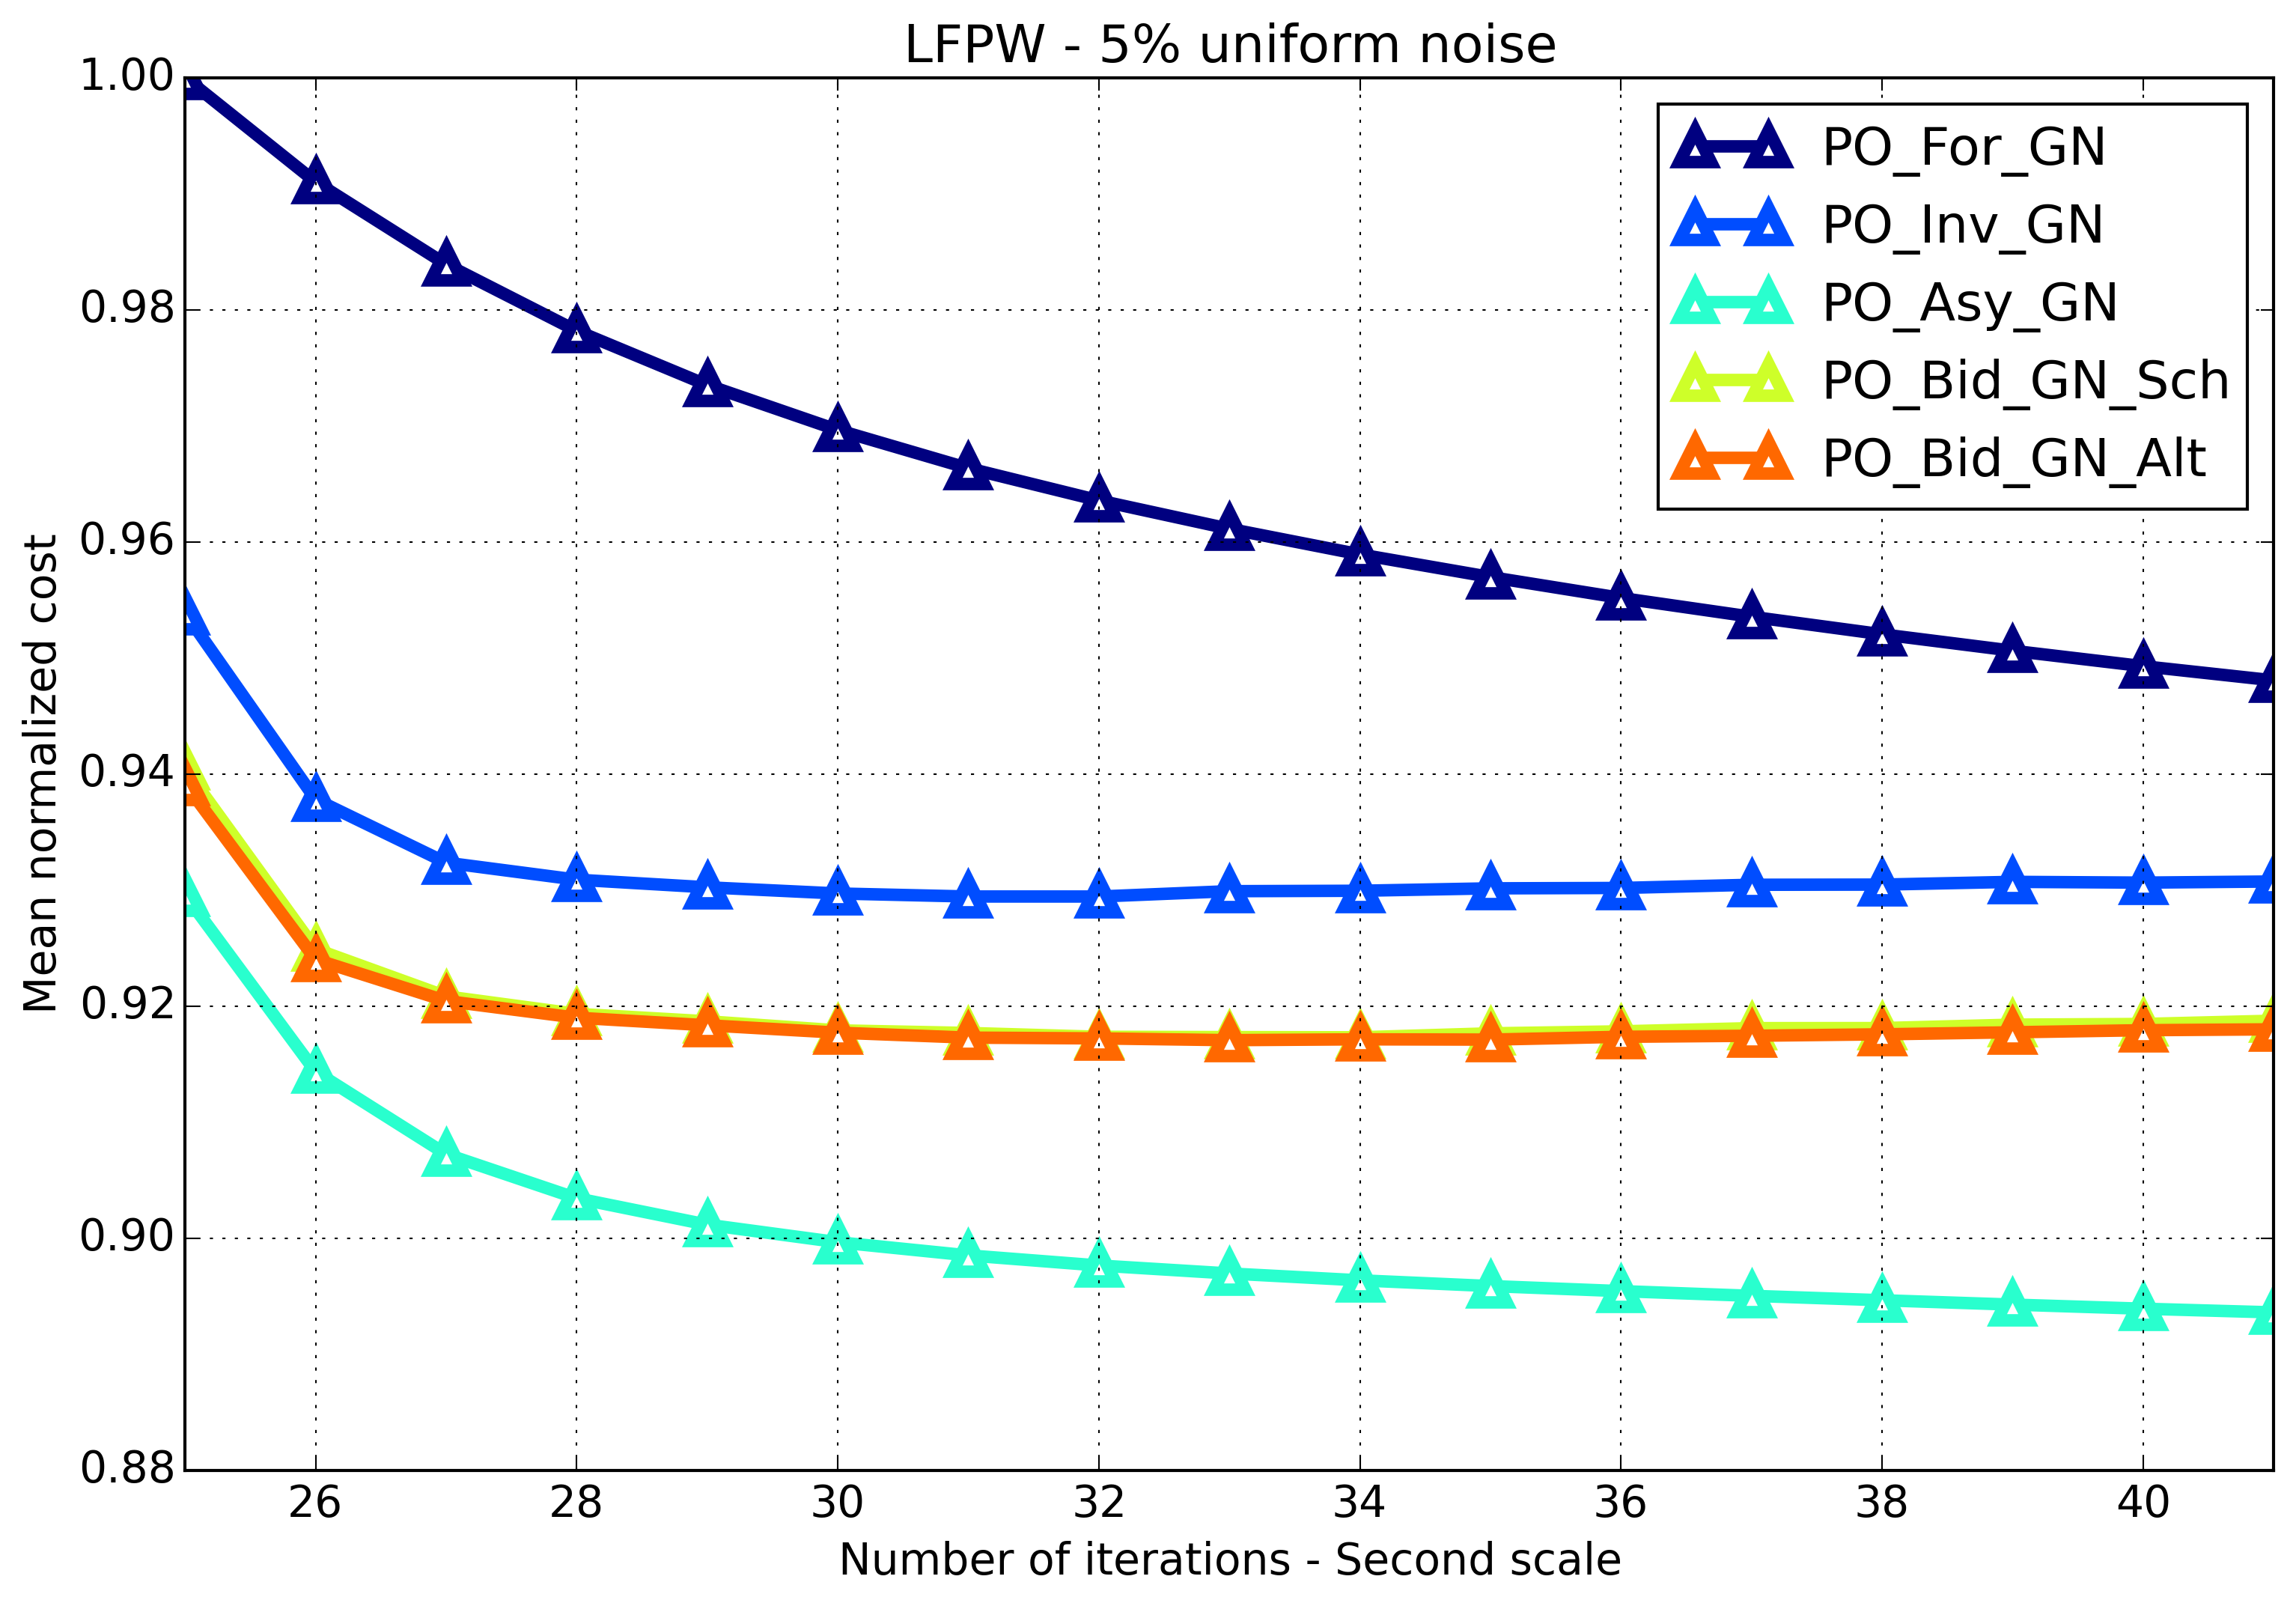
\includegraphics[width=\textwidth]{experiments/algorithms/po_gn/mean_cost_vs_iters2_po_gn_5.png}
	    \caption{Mean normalized cost vs number of second scale iterations graph on the LFPW test dataset for all Project-Out Gauss-Newton algorithms initialized with $5\%$ uniform noise.}
	    \label{fig:mean_cost_vs_iters2_po_gn_5}
	\end{subfigure}
	\label{fig:po_gn_5}
	\caption{}
\end{figure*}


% \subsubsection{Project-Out Newton algorithms}

% \begin{figure}[h!]
%     \centering
%     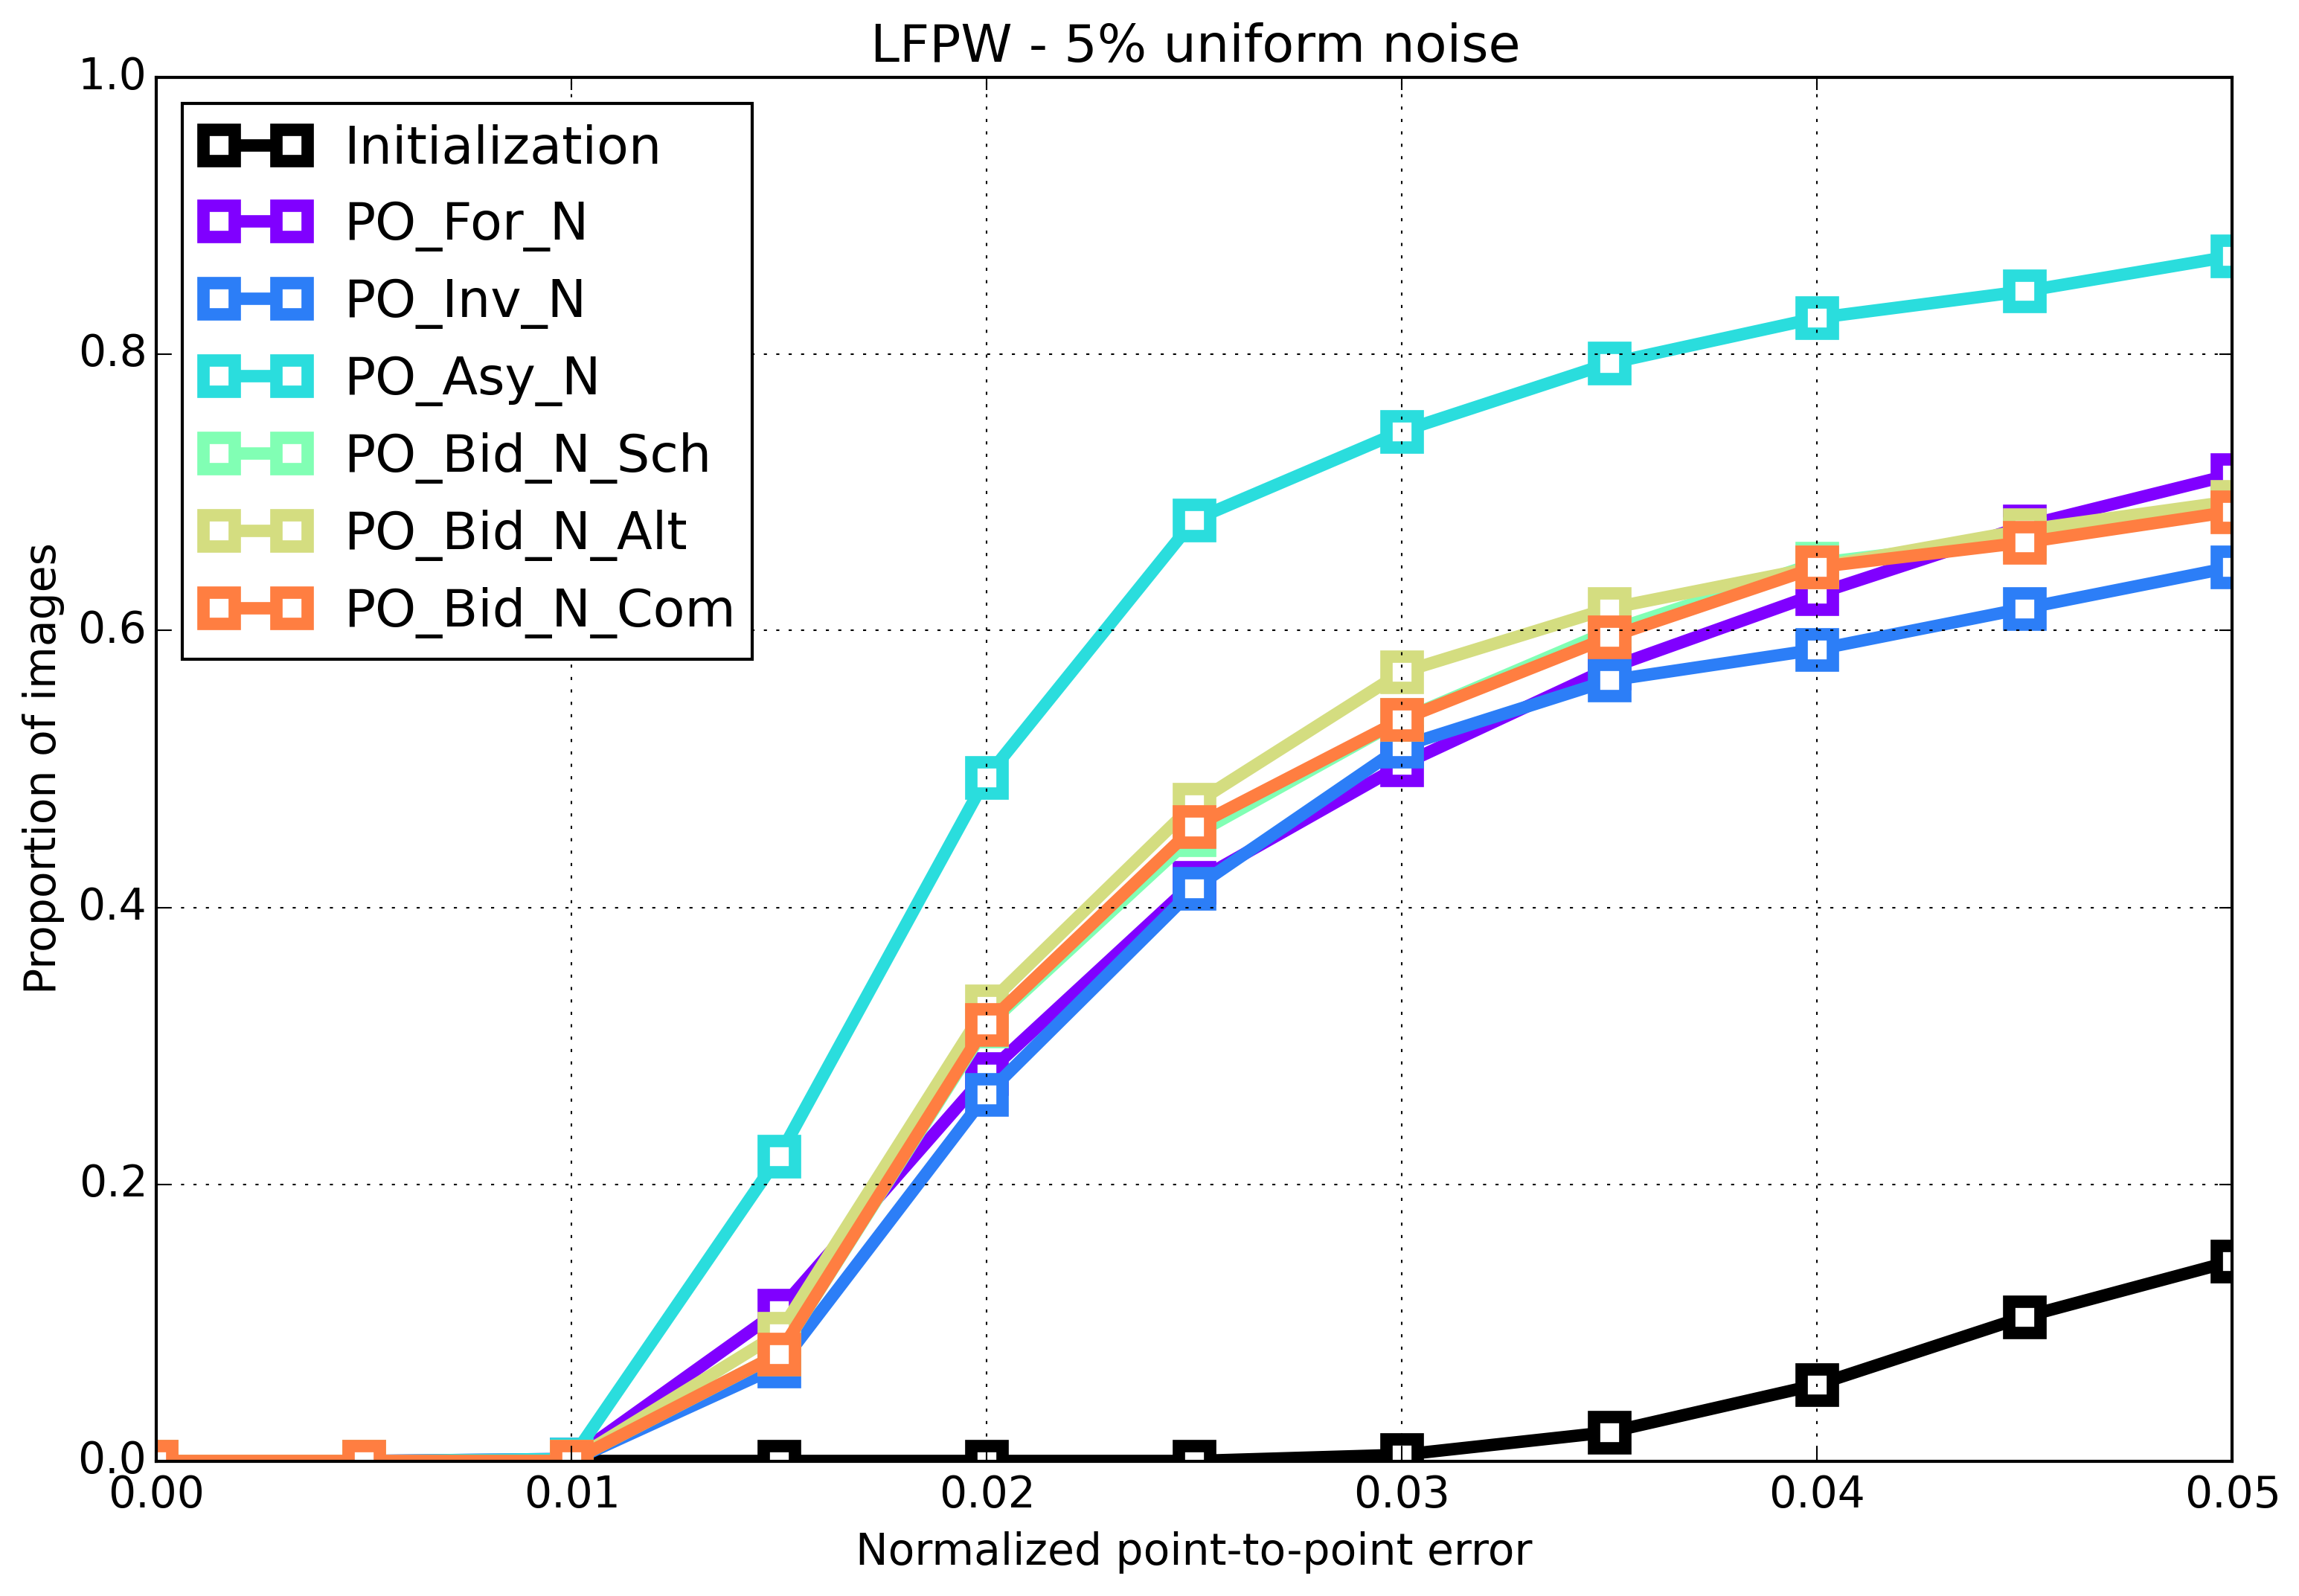
\includegraphics[width=0.50\textwidth]{experiments/algorithms/po_n/ced_po_n_5.png}
%     \caption{CED graph on the LFPW test dataset for all Project-Out Newton algorithms initialized with $4$\% uniform noise.}
%     \label{fig:ced_po_gn_4}
% \end{figure}

% \begin{figure}[h!]
%     \centering
%     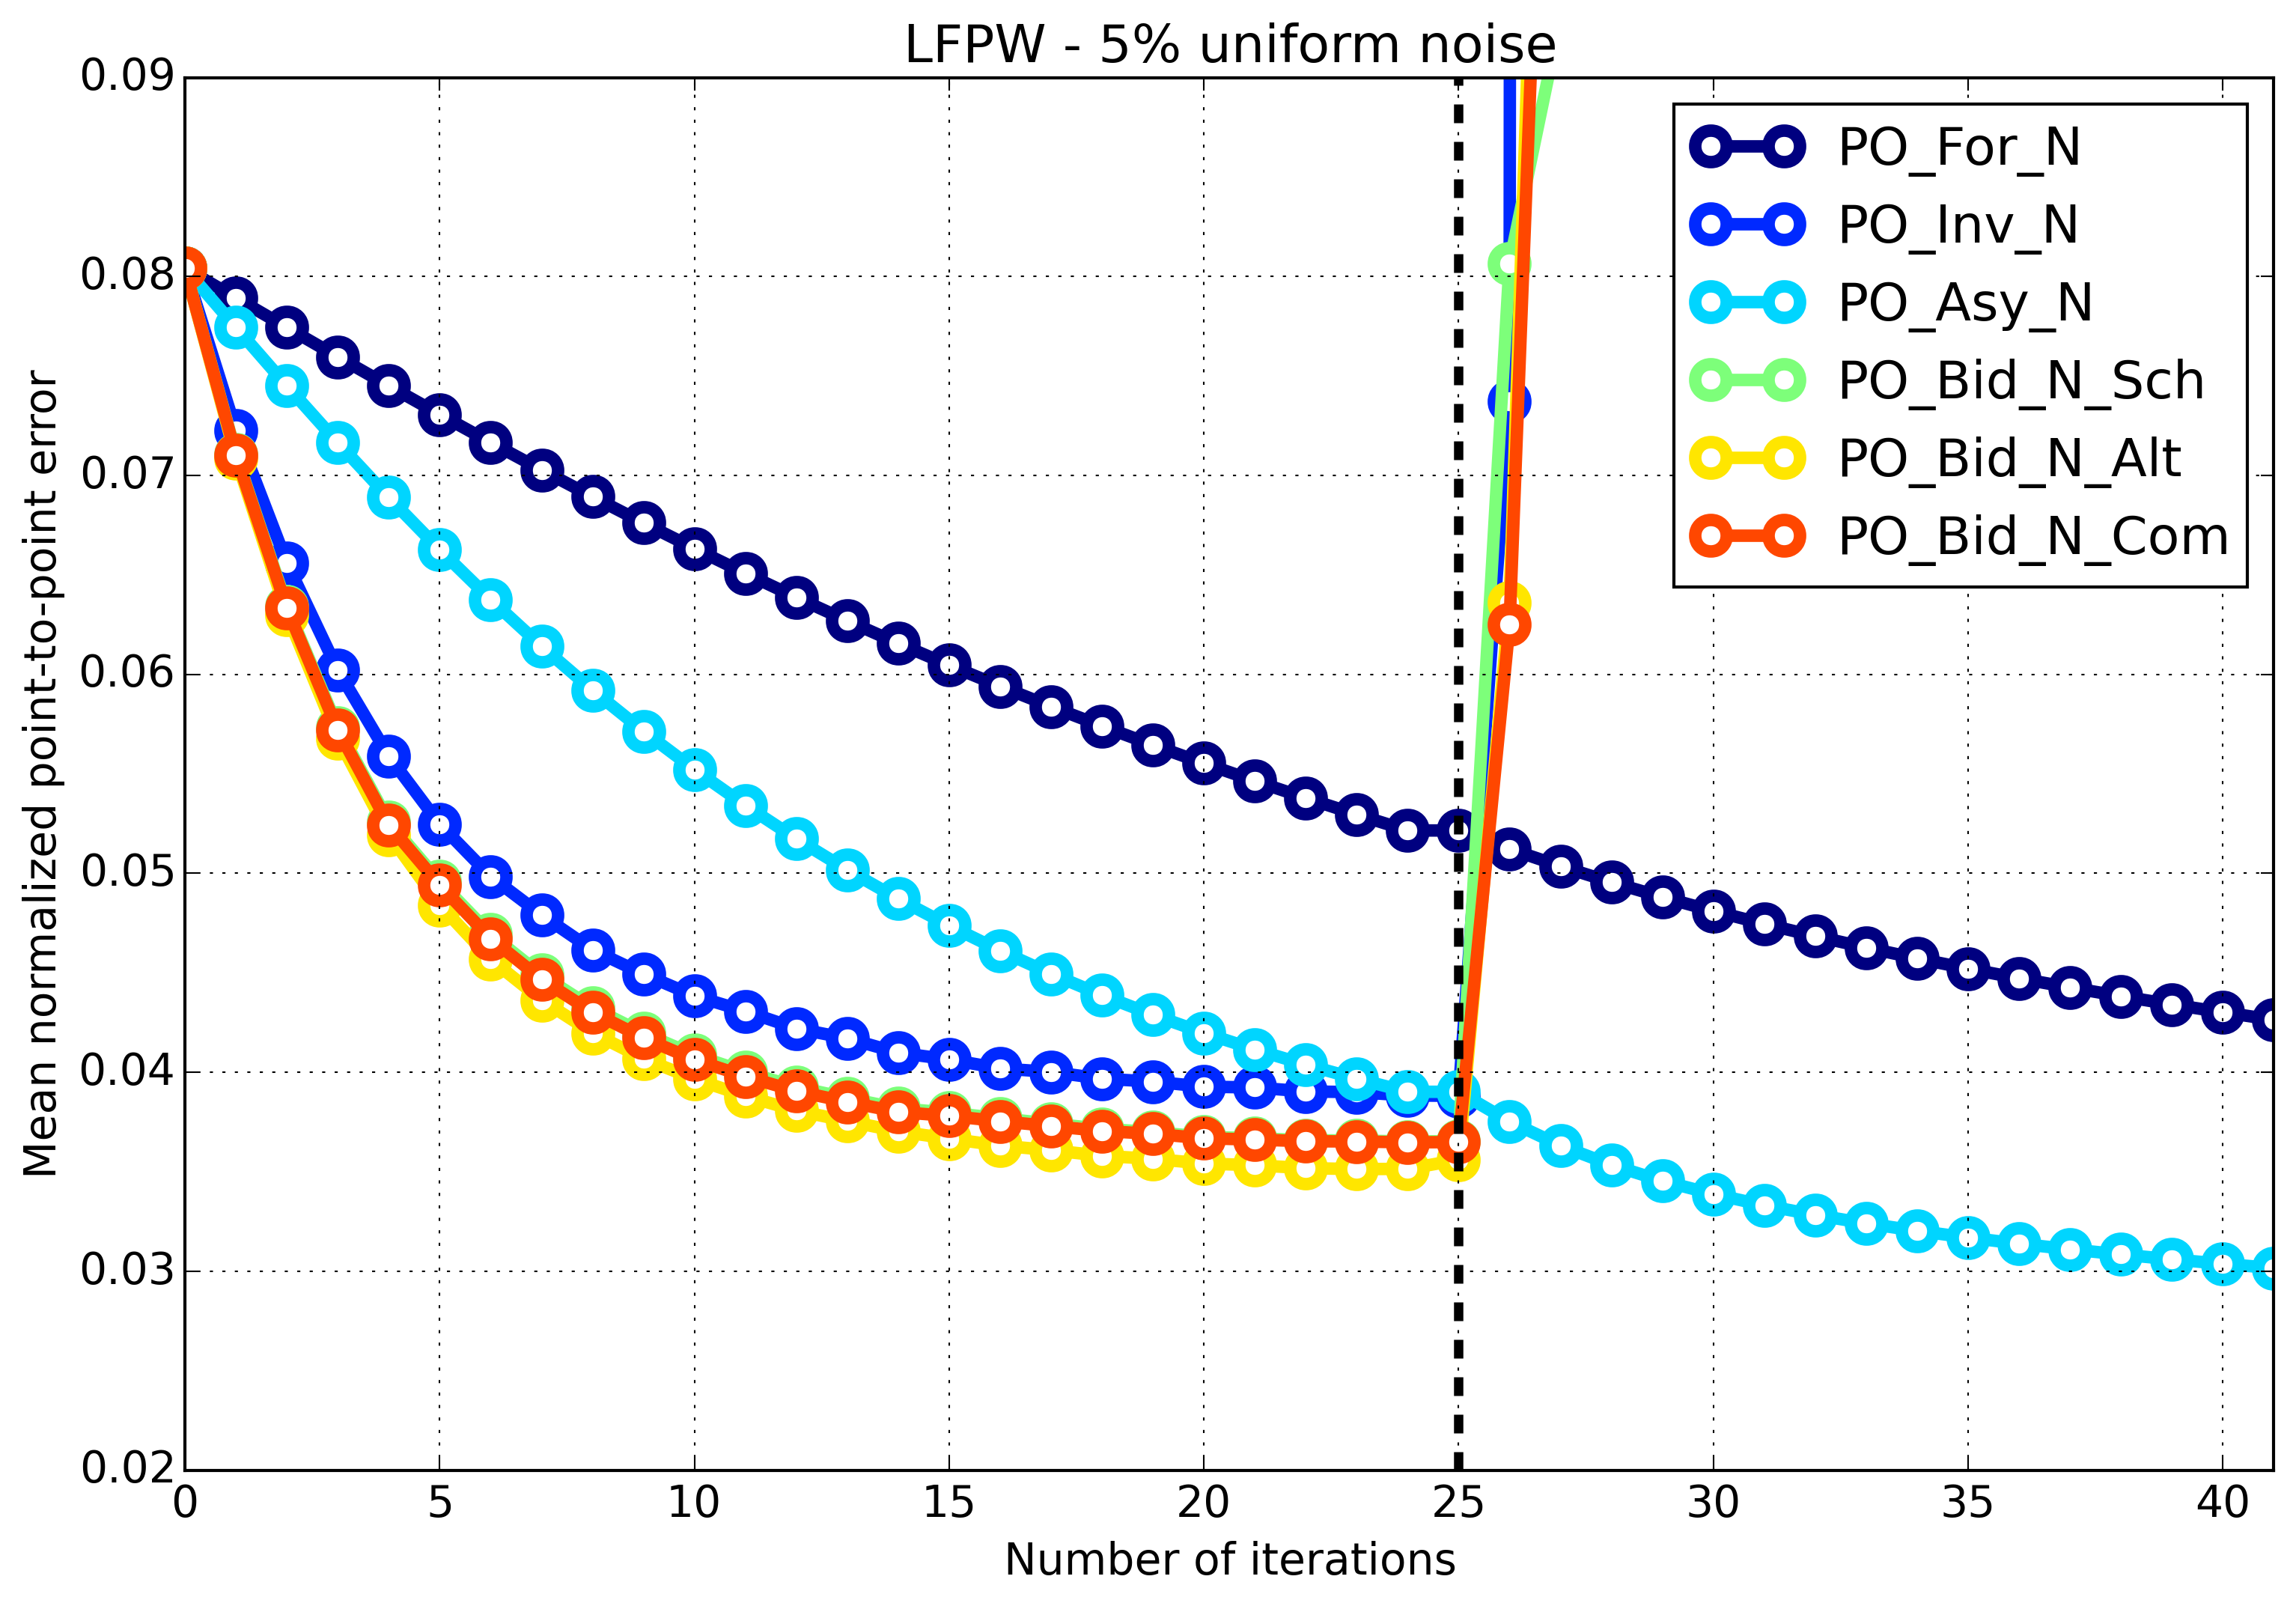
\includegraphics[width=0.50\textwidth]{experiments/algorithms/po_n/mean_error_vs_iters_po_n_5.png}
%     \caption{Mean normalized point-to-point error vs number of iterations graph on the LFPW test dataset for all Project-Out Newton algorithms initialized with $4$\% uniform noise.}
%     \label{fig:mean_error_vs_iters_po_n_4}
% \end{figure}

% \begin{figure}[h!]
%     \centering
%     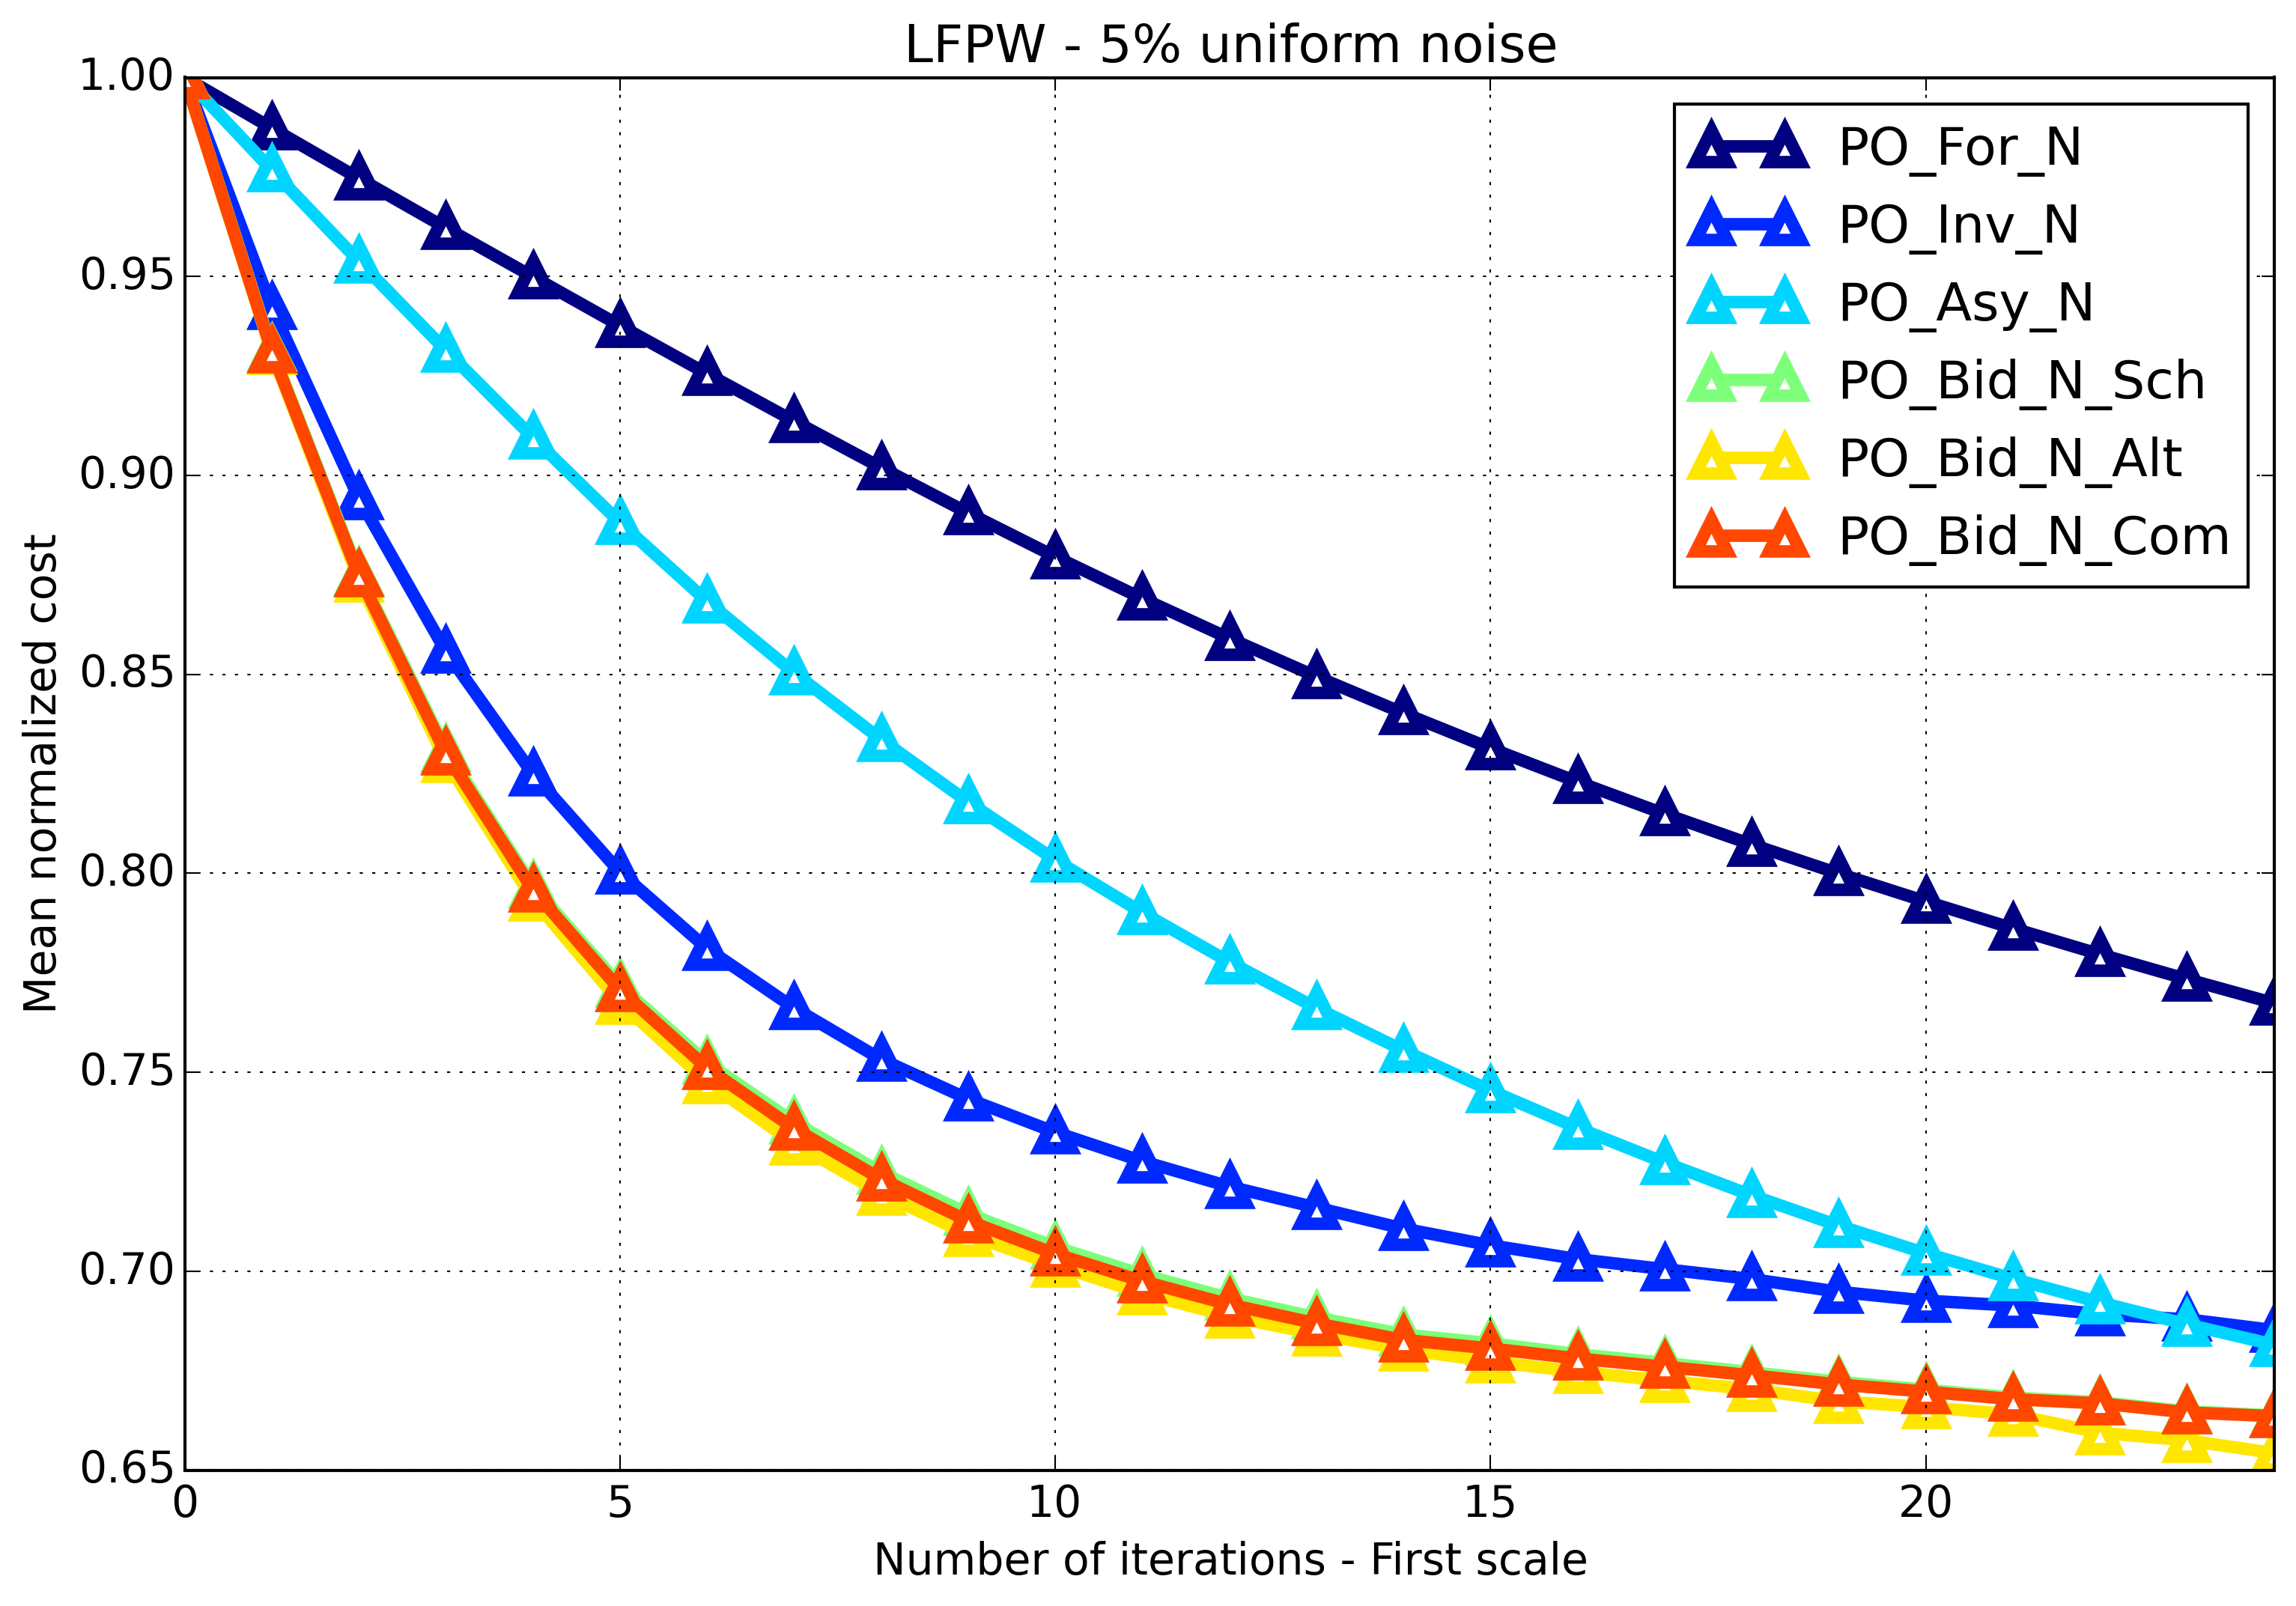
\includegraphics[width=0.50\textwidth]{experiments/algorithms/po_n/mean_cost_vs_iters1_po_n_5.png}
%     \caption{Mean normalized cost vs number of first scale iterations graph on the LFPW test dataset for all Project-Out Newton algorithms initialized with $4$\% uniform noise.}
%     \label{fig:mean_cost_vs_iters1_po_n_4}
% \end{figure}

% \begin{figure}[h!]
%     \centering
%     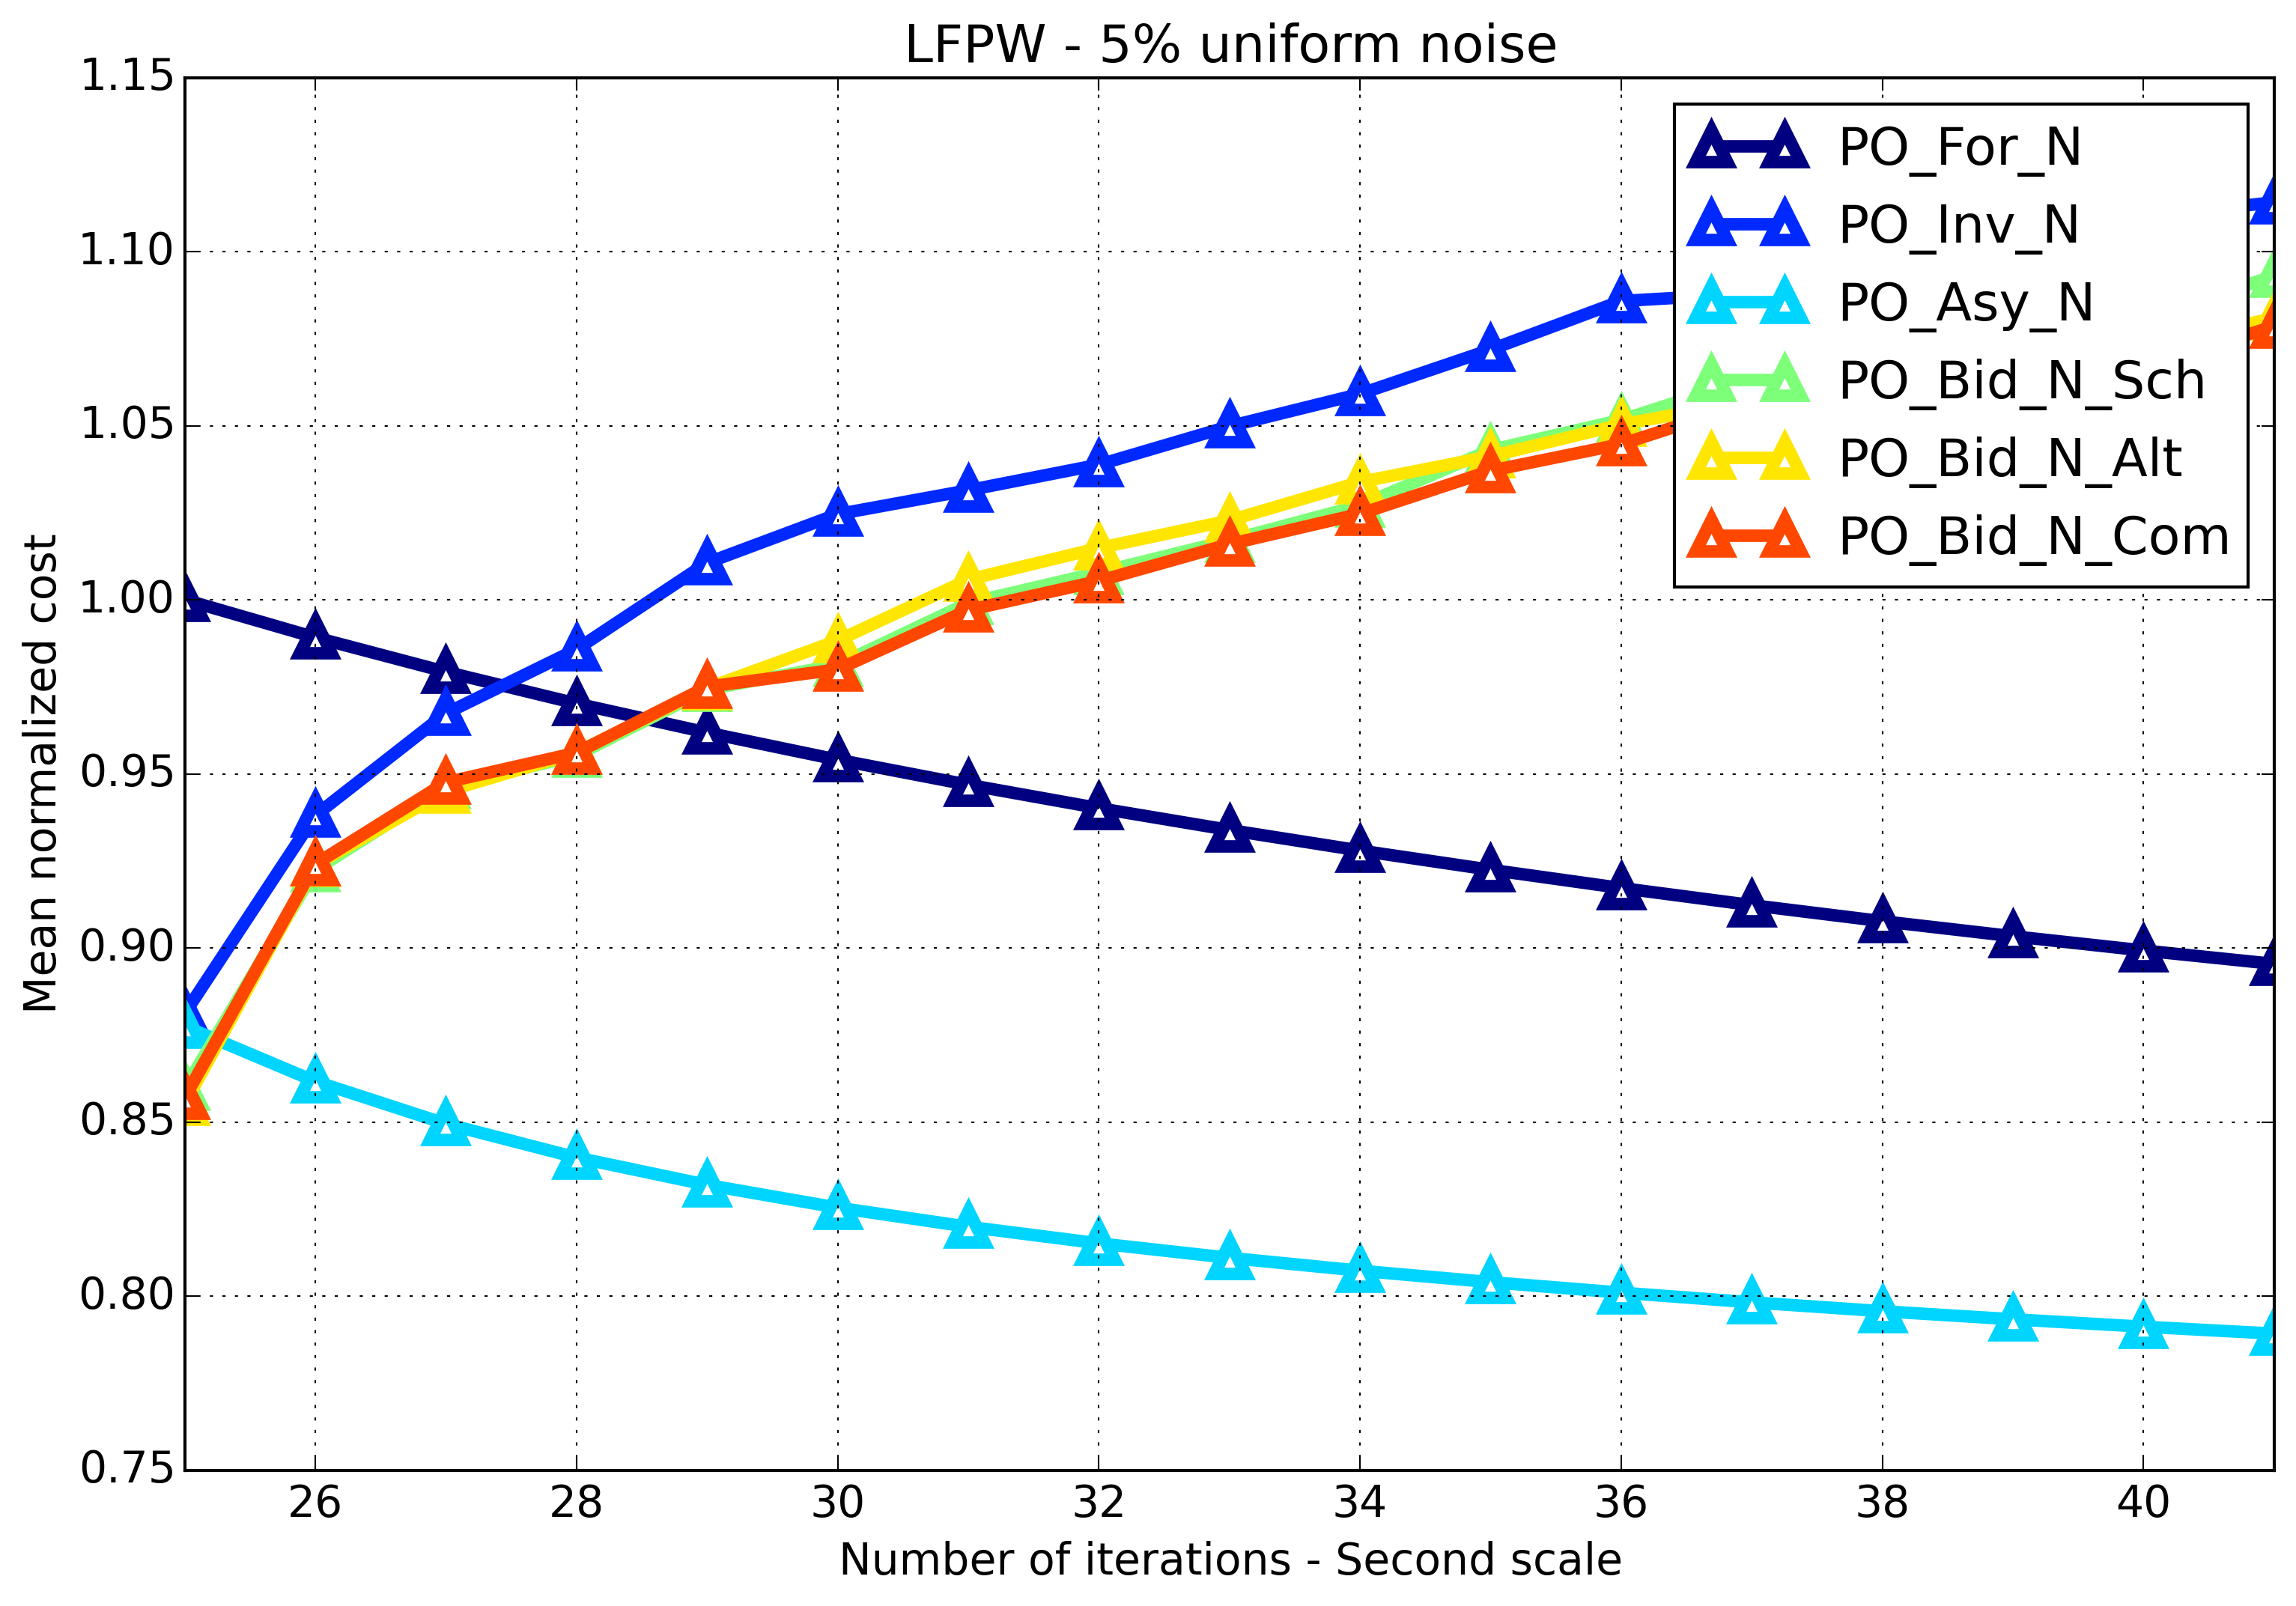
\includegraphics[width=0.50\textwidth]{experiments/algorithms/po_n/mean_cost_vs_iters2_po_n_5.png}
%     \caption{Mean normalized cost vs number of second scale iterations graph on the LFPW test dataset for all Project-Out Newton algorithms initialized with $4$\% uniform noise.}
%     \label{fig:mean_cost_vs_iters2_po_n_4}
% \end{figure}

\subsubsection*{Wiberg}

\begin{figure*}[h!]
	\centering
	\begin{subfigure}{0.48\textwidth}
	    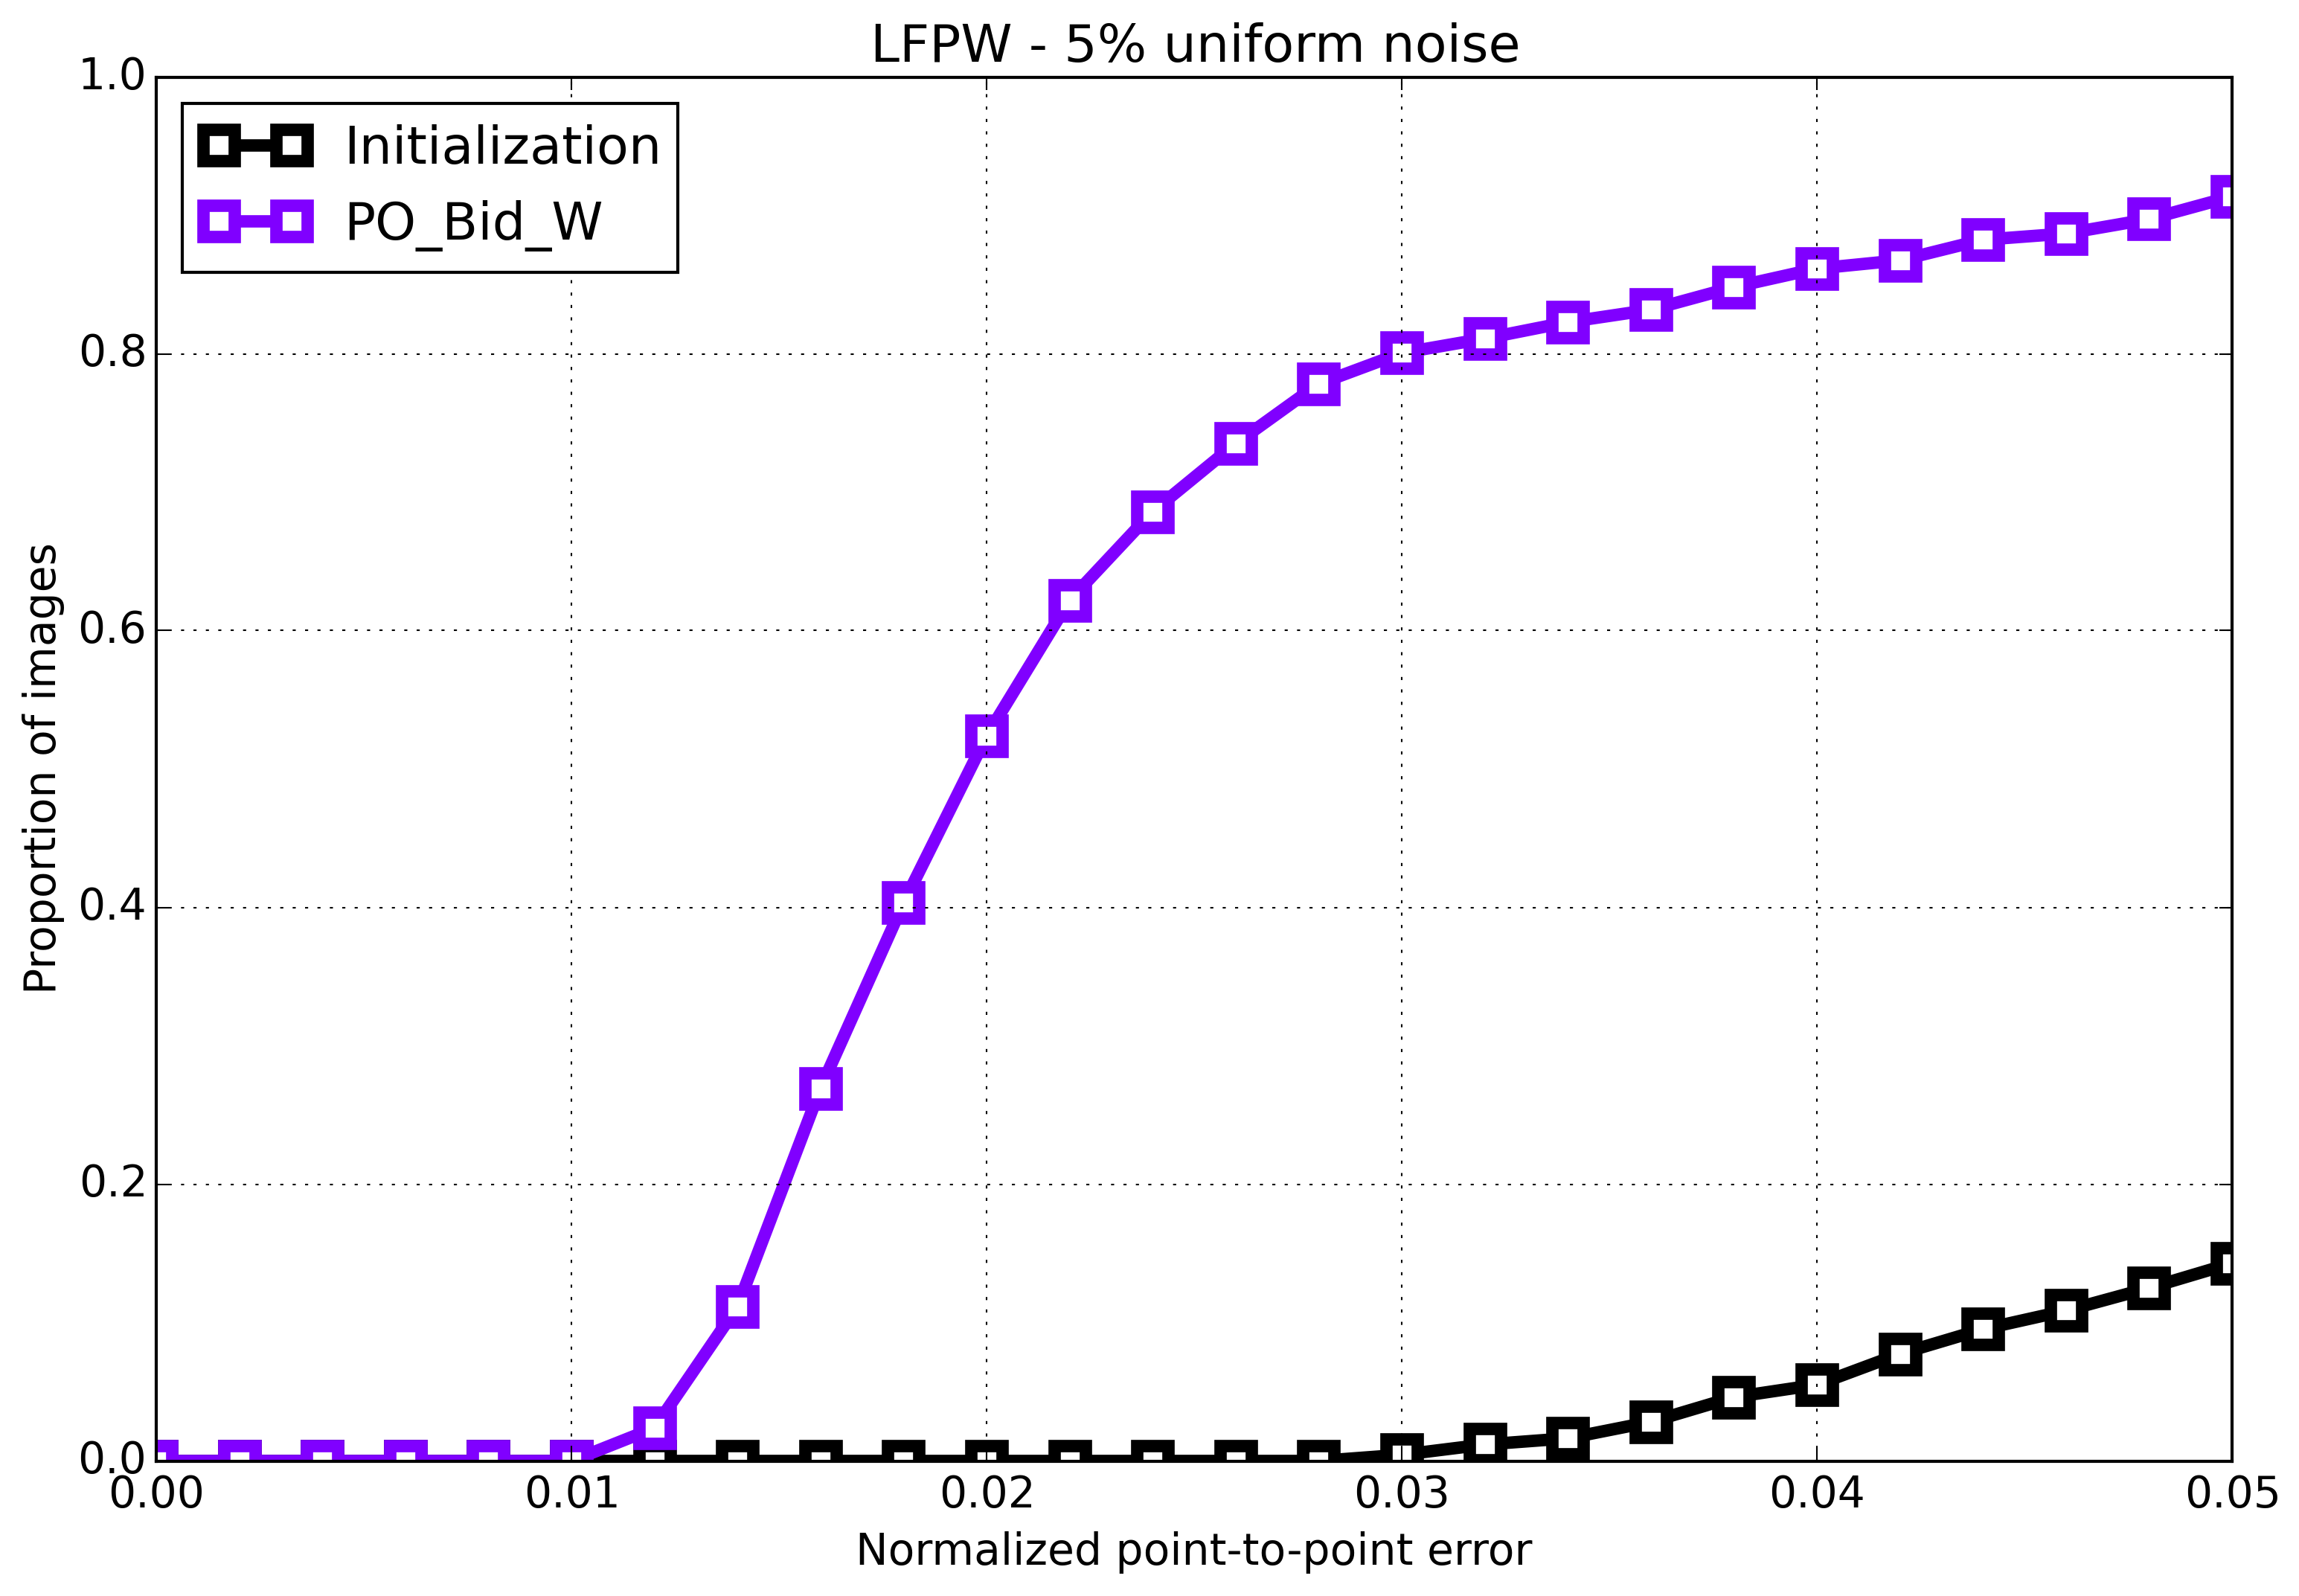
\includegraphics[width=\textwidth]{experiments/algorithms/po_w/ced_po_w_5.png}
	    \caption{Cumulative Error Distribution graph on the LFPW test dataset for all Project-Out Wiberg algorithms initialized with $5\%$ uniform noise.}
	    \label{fig:ced_po_w_5}
	\end{subfigure}
	\hfill
	\begin{subfigure}{0.48\textwidth}
	    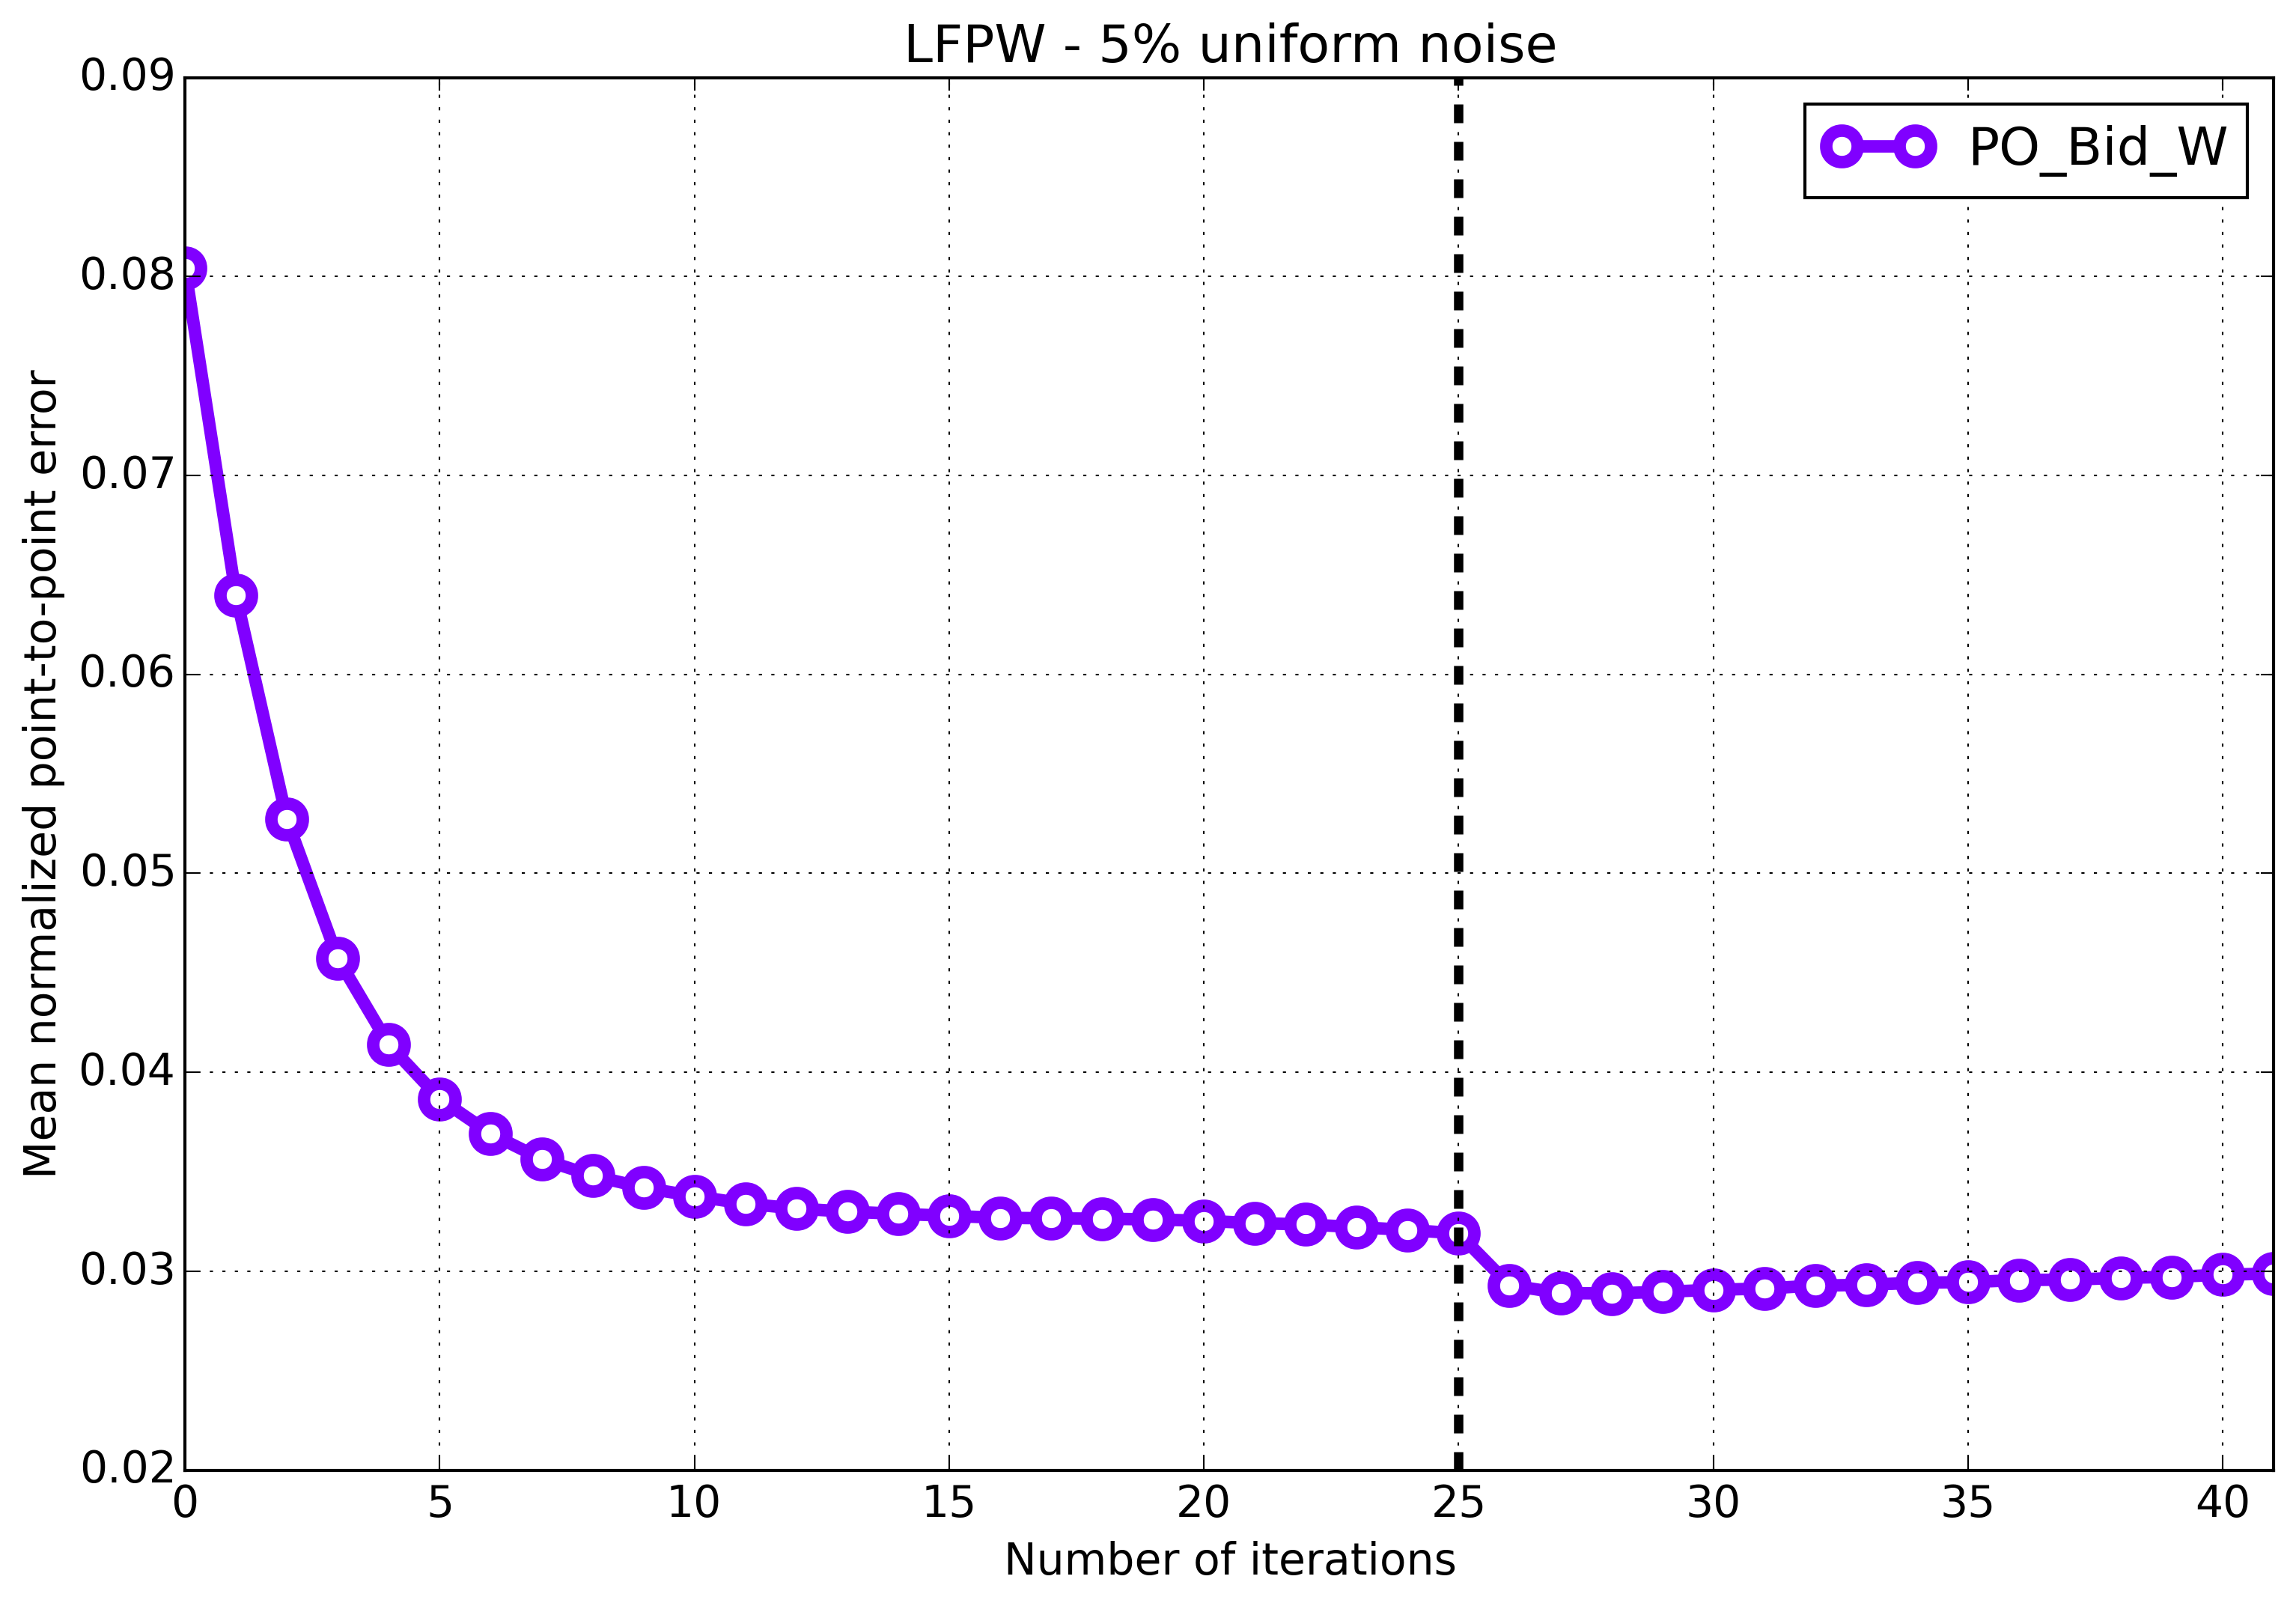
\includegraphics[width=\textwidth]{experiments/algorithms/po_w/mean_error_vs_iters_po_w_5.png}
	    \caption{Mean normalized point-to-point error vs number of iterations graph on the LFPW test dataset for all Project-Out Wiberg algorithms initialized with $5\%$ uniform noise.}
	    \label{fig:mean_error_vs_iters_po_w_5}
	\end{subfigure}
	\par\medskip
	\begin{subfigure}{0.48\textwidth}
	    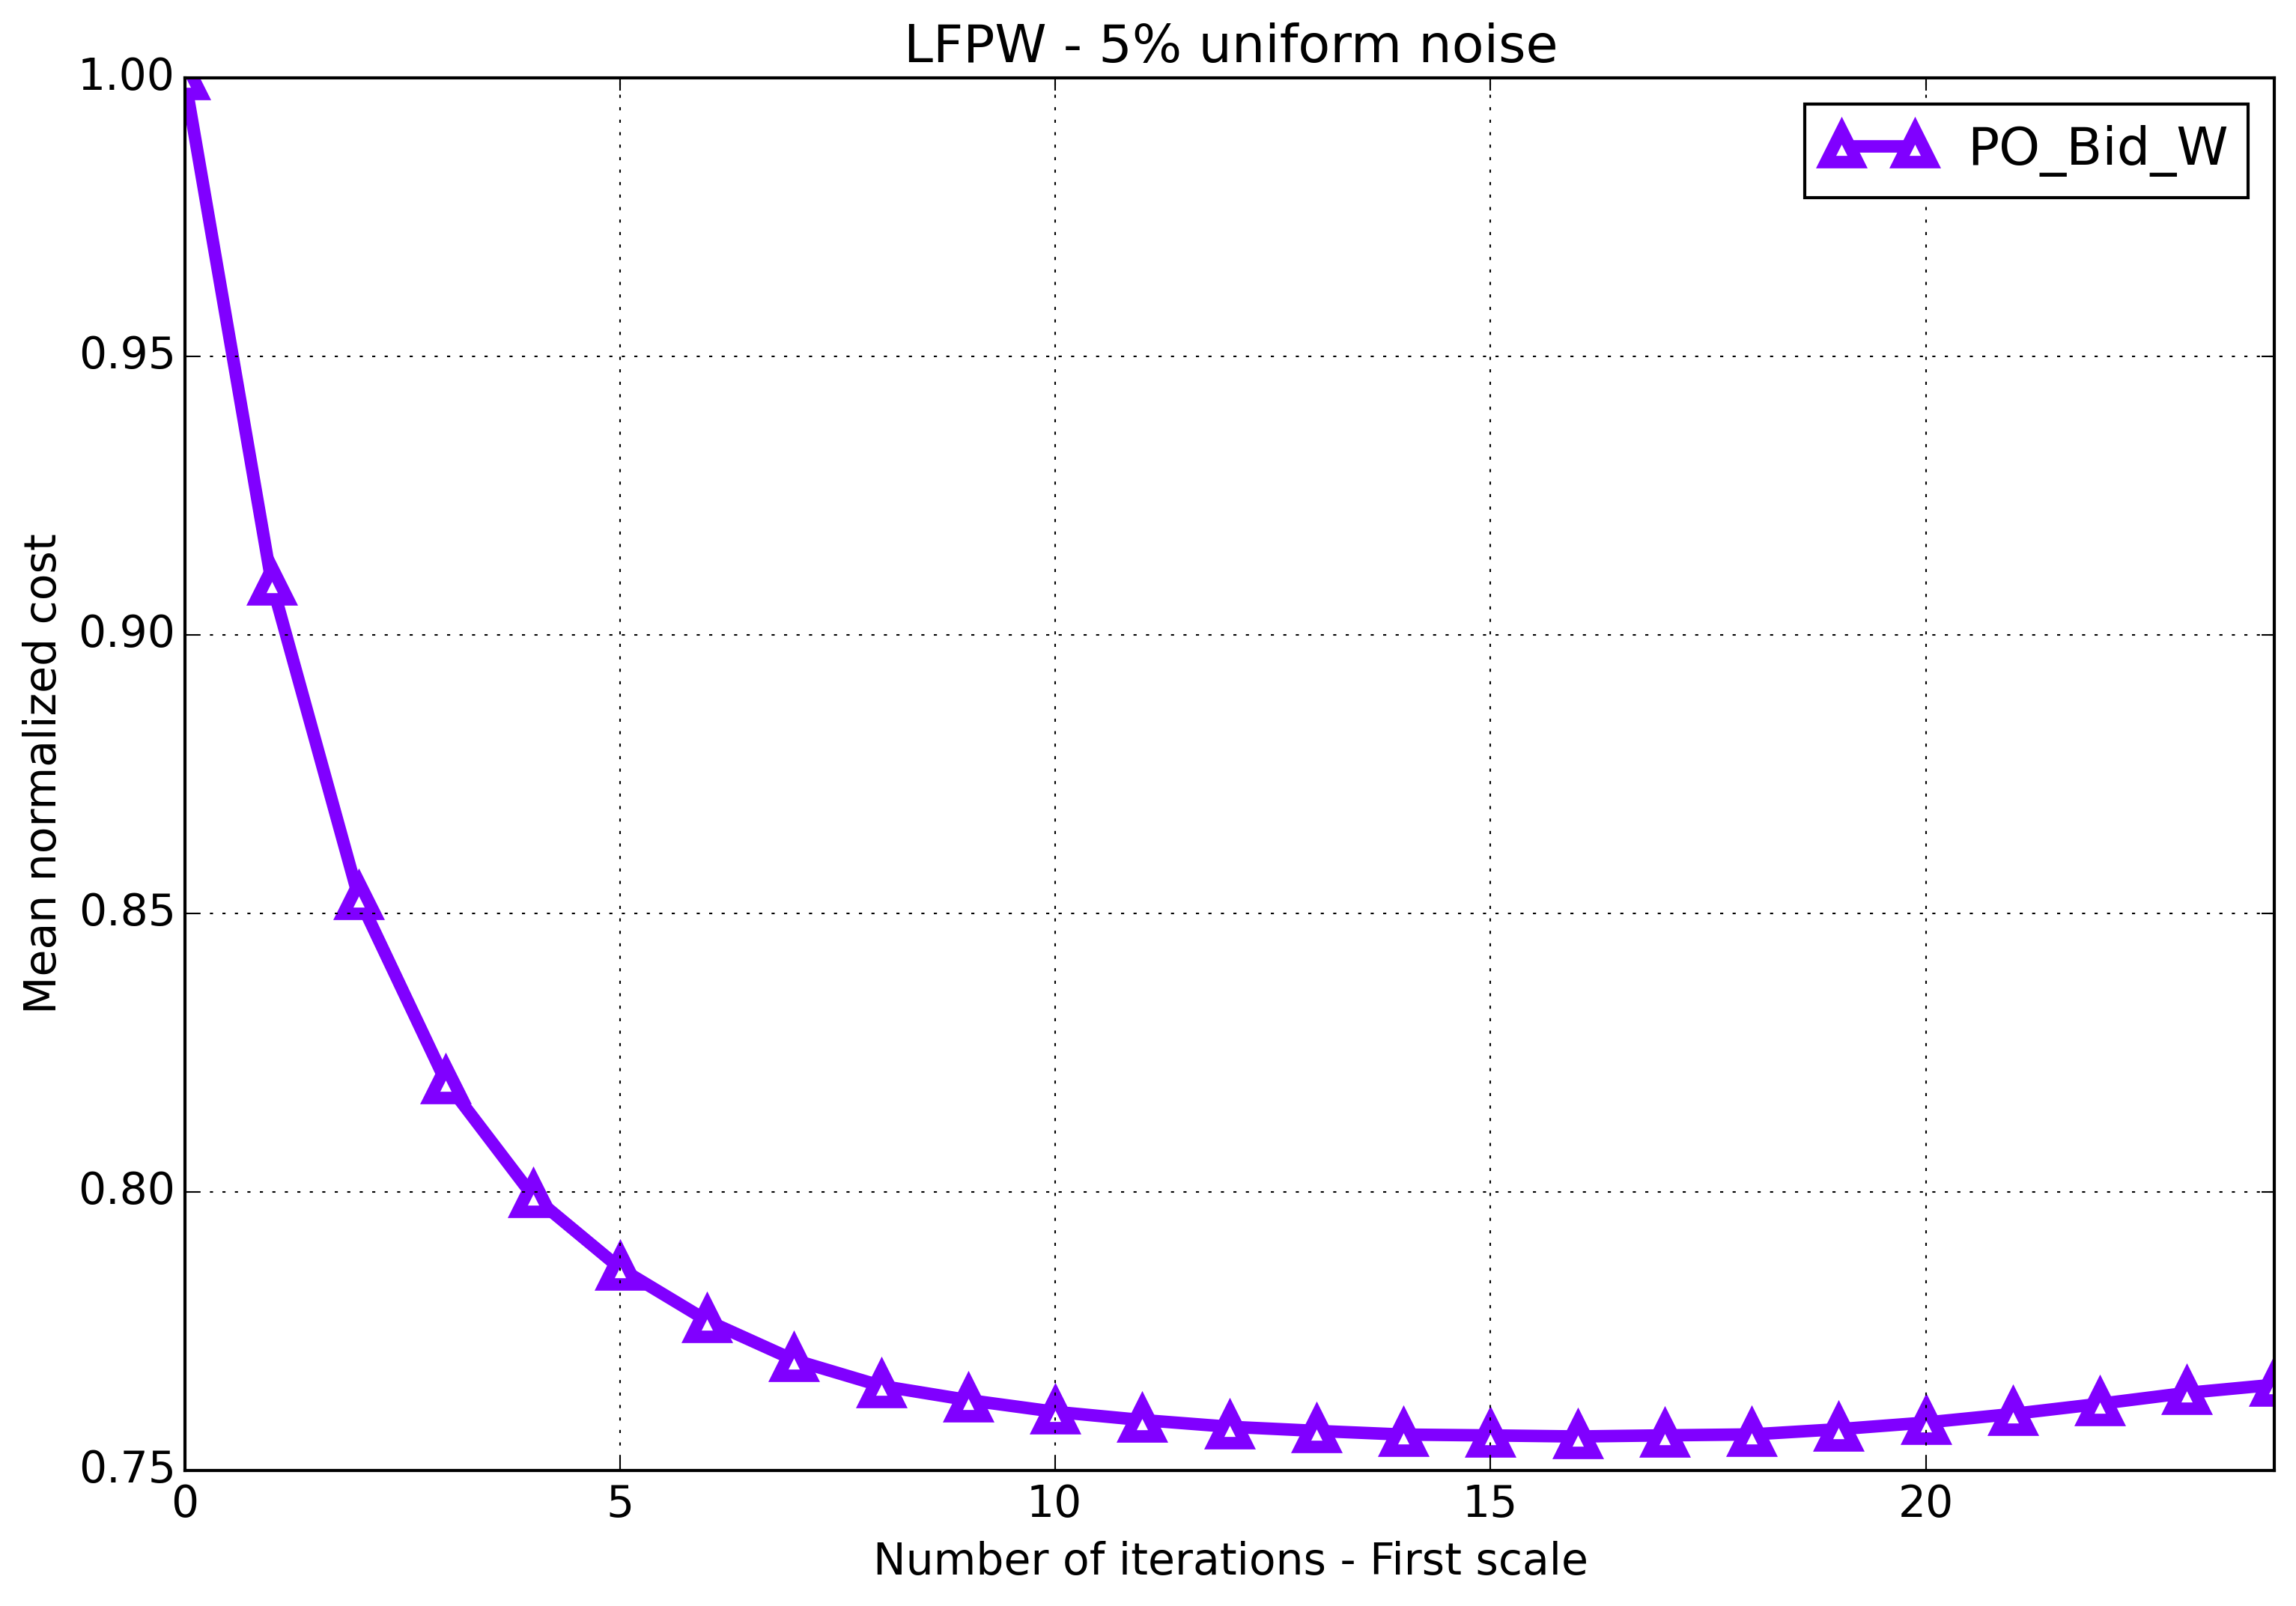
\includegraphics[width=\textwidth]{experiments/algorithms/po_w/mean_cost_vs_iters1_po_w_5.png}
	    \caption{Mean normalized cost vs number of first scale iterations graph on the LFPW test dataset for all Project-Out Wiberg algorithms initialized with $5\%$ uniform noise.}
	    \label{fig:mean_cost_vs_iters1_po_w_5}
	\end{subfigure}
	\hfill
	\begin{subfigure}{0.48\textwidth}
	    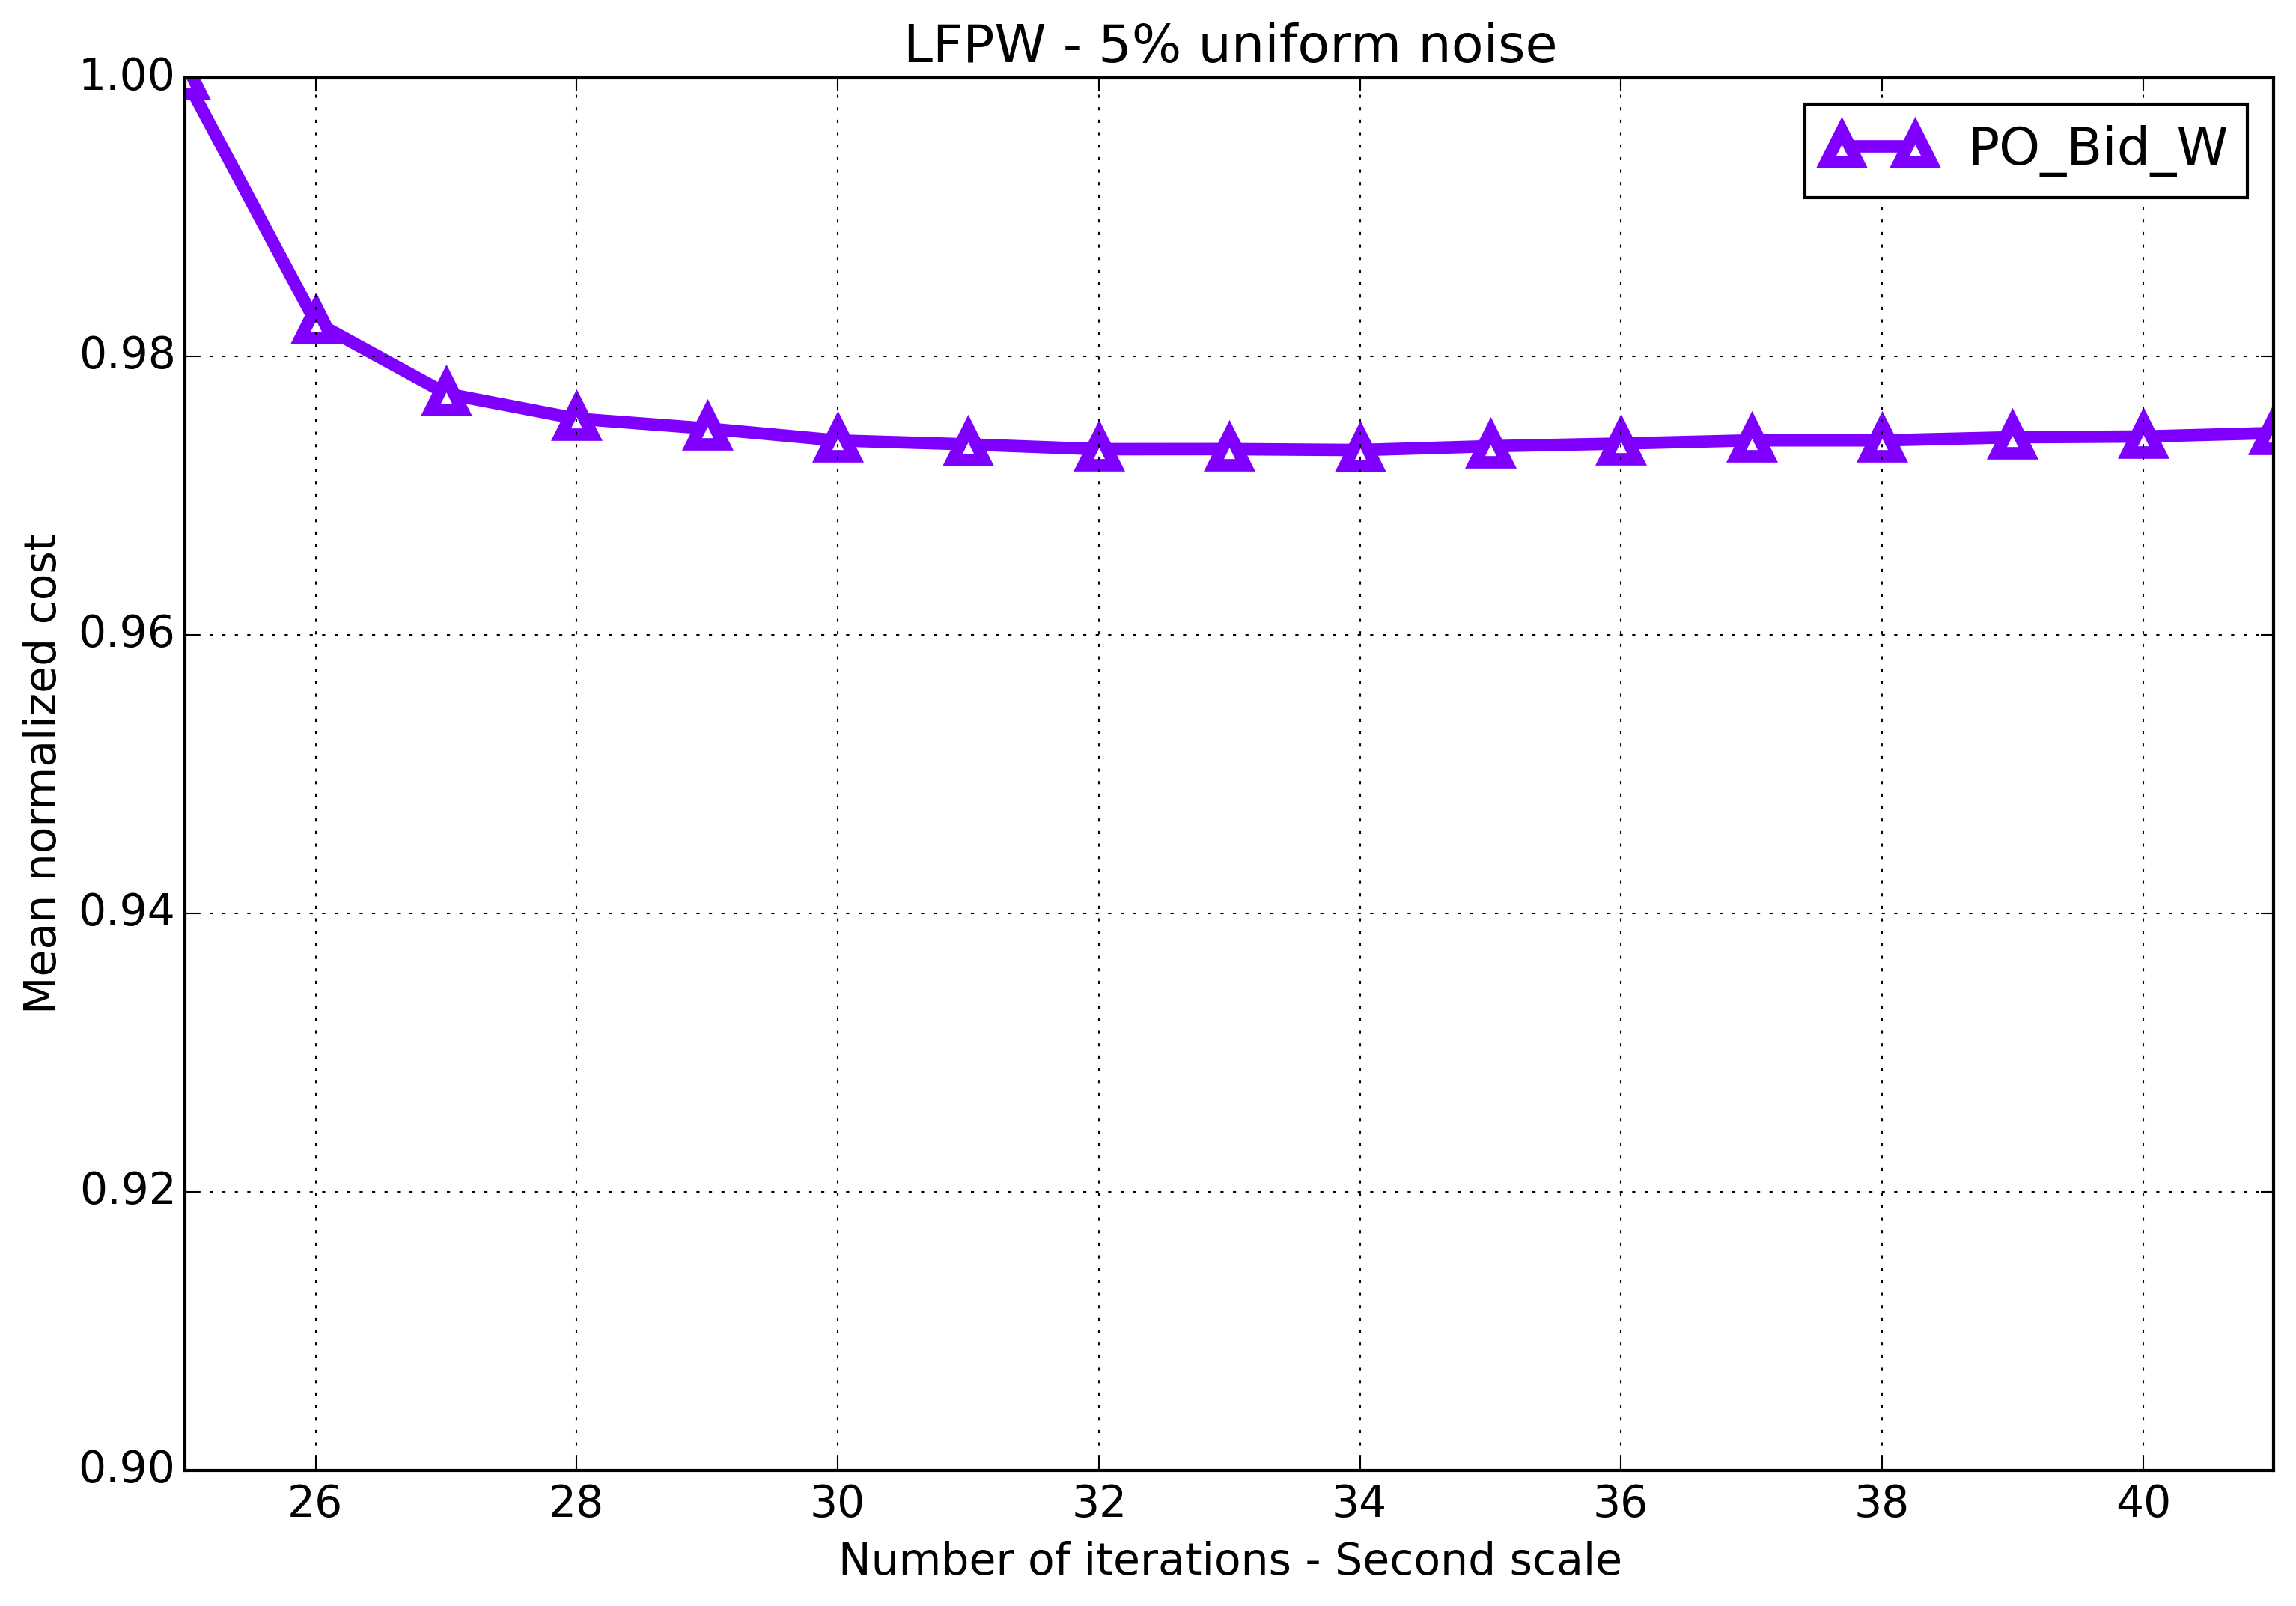
\includegraphics[width=\textwidth]{experiments/algorithms/po_w/mean_cost_vs_iters2_po_w_5.png}
	    \caption{Mean normalized cost vs number of second scale iterations graph on the LFPW test dataset for all Project-Out Wiberg algorithms initialized with $5\%$ uniform noise.}
	    \label{fig:mean_cost_vs_iters2_po_w_5}
	\end{subfigure}
	\label{fig:po_w_5}
	\caption{}
\end{figure*}


% \begin{figure}[h!]
%     \centering
%     \includegraphics[width=0.50\textwidth]{experiments/algorithms/ssd_gn/ced_ssd_gn_4.png}
%     \caption{CED graph on the LFPW test dataset for all SSD Gauss-Newton algorithms initialized with $4$\% of uniform noise.}
%     \label{fig:ced_po_asymmetric_gn_4}
% \end{figure}




% \begin{figure}[h!]
%     \centering
%     \includegraphics[width=0.50\textwidth]{experiments/algorithms/ssd_gn/mean_error_vs_iters_ssd_gn_4.png}
%     \caption{Mean normalized point-to-point error vs number of iterations graph on the LFPW test dataset for all SSD Gauss-Newton algorithms initialized with $4$\% of uniform noise}
%     \label{fig:mean_error_vs_iters_po_asymmetric_gn_4}
% \end{figure}


\subsubsection{Weighted Bayesian project-out}

\begin{figure}[h!]
	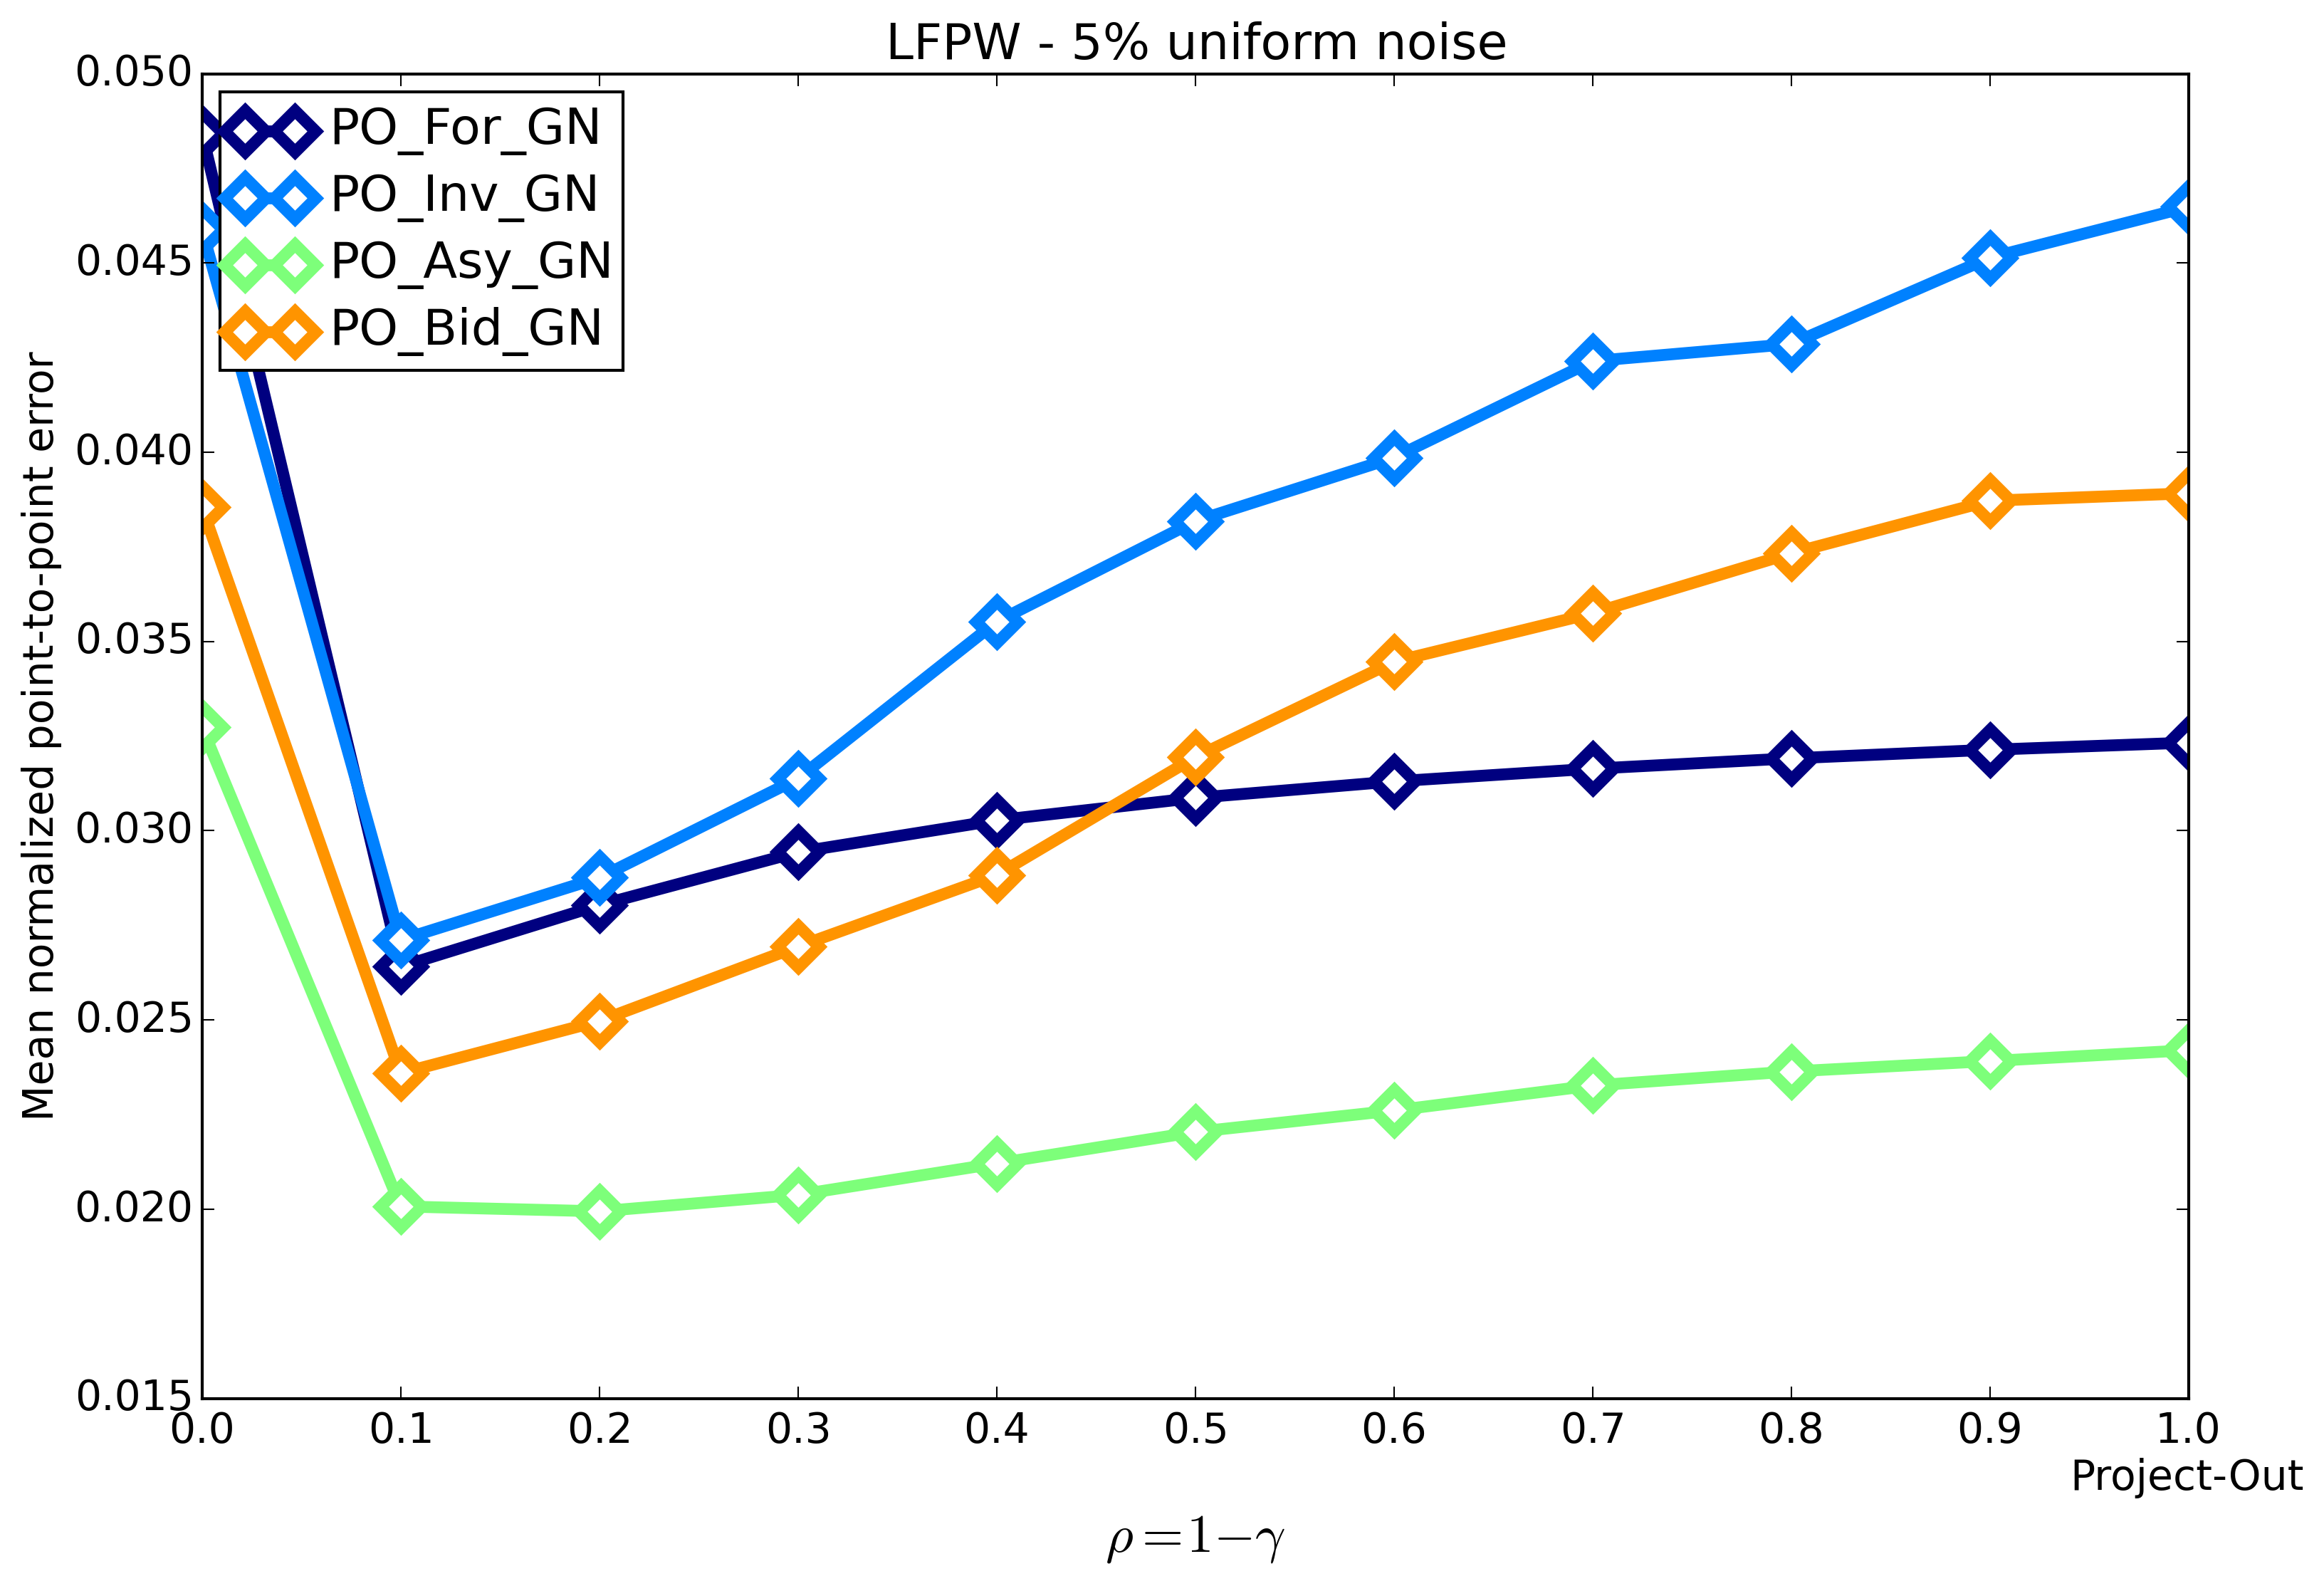
\includegraphics[width=0.48\textwidth]{experiments/rho/mean_error_vs_rho_5.png}
    \caption{Mean normalized point-to-point error vs rho on the LFPW test dataset for all PO Gauss-Newton algorithms initialized with $5\%$ uniform noise.}
    \label{fig:ced_ssd_gn_5}
\end{figure}

\subsubsection{Optimal asymmetric composition}

\begin{figure}[h!]
    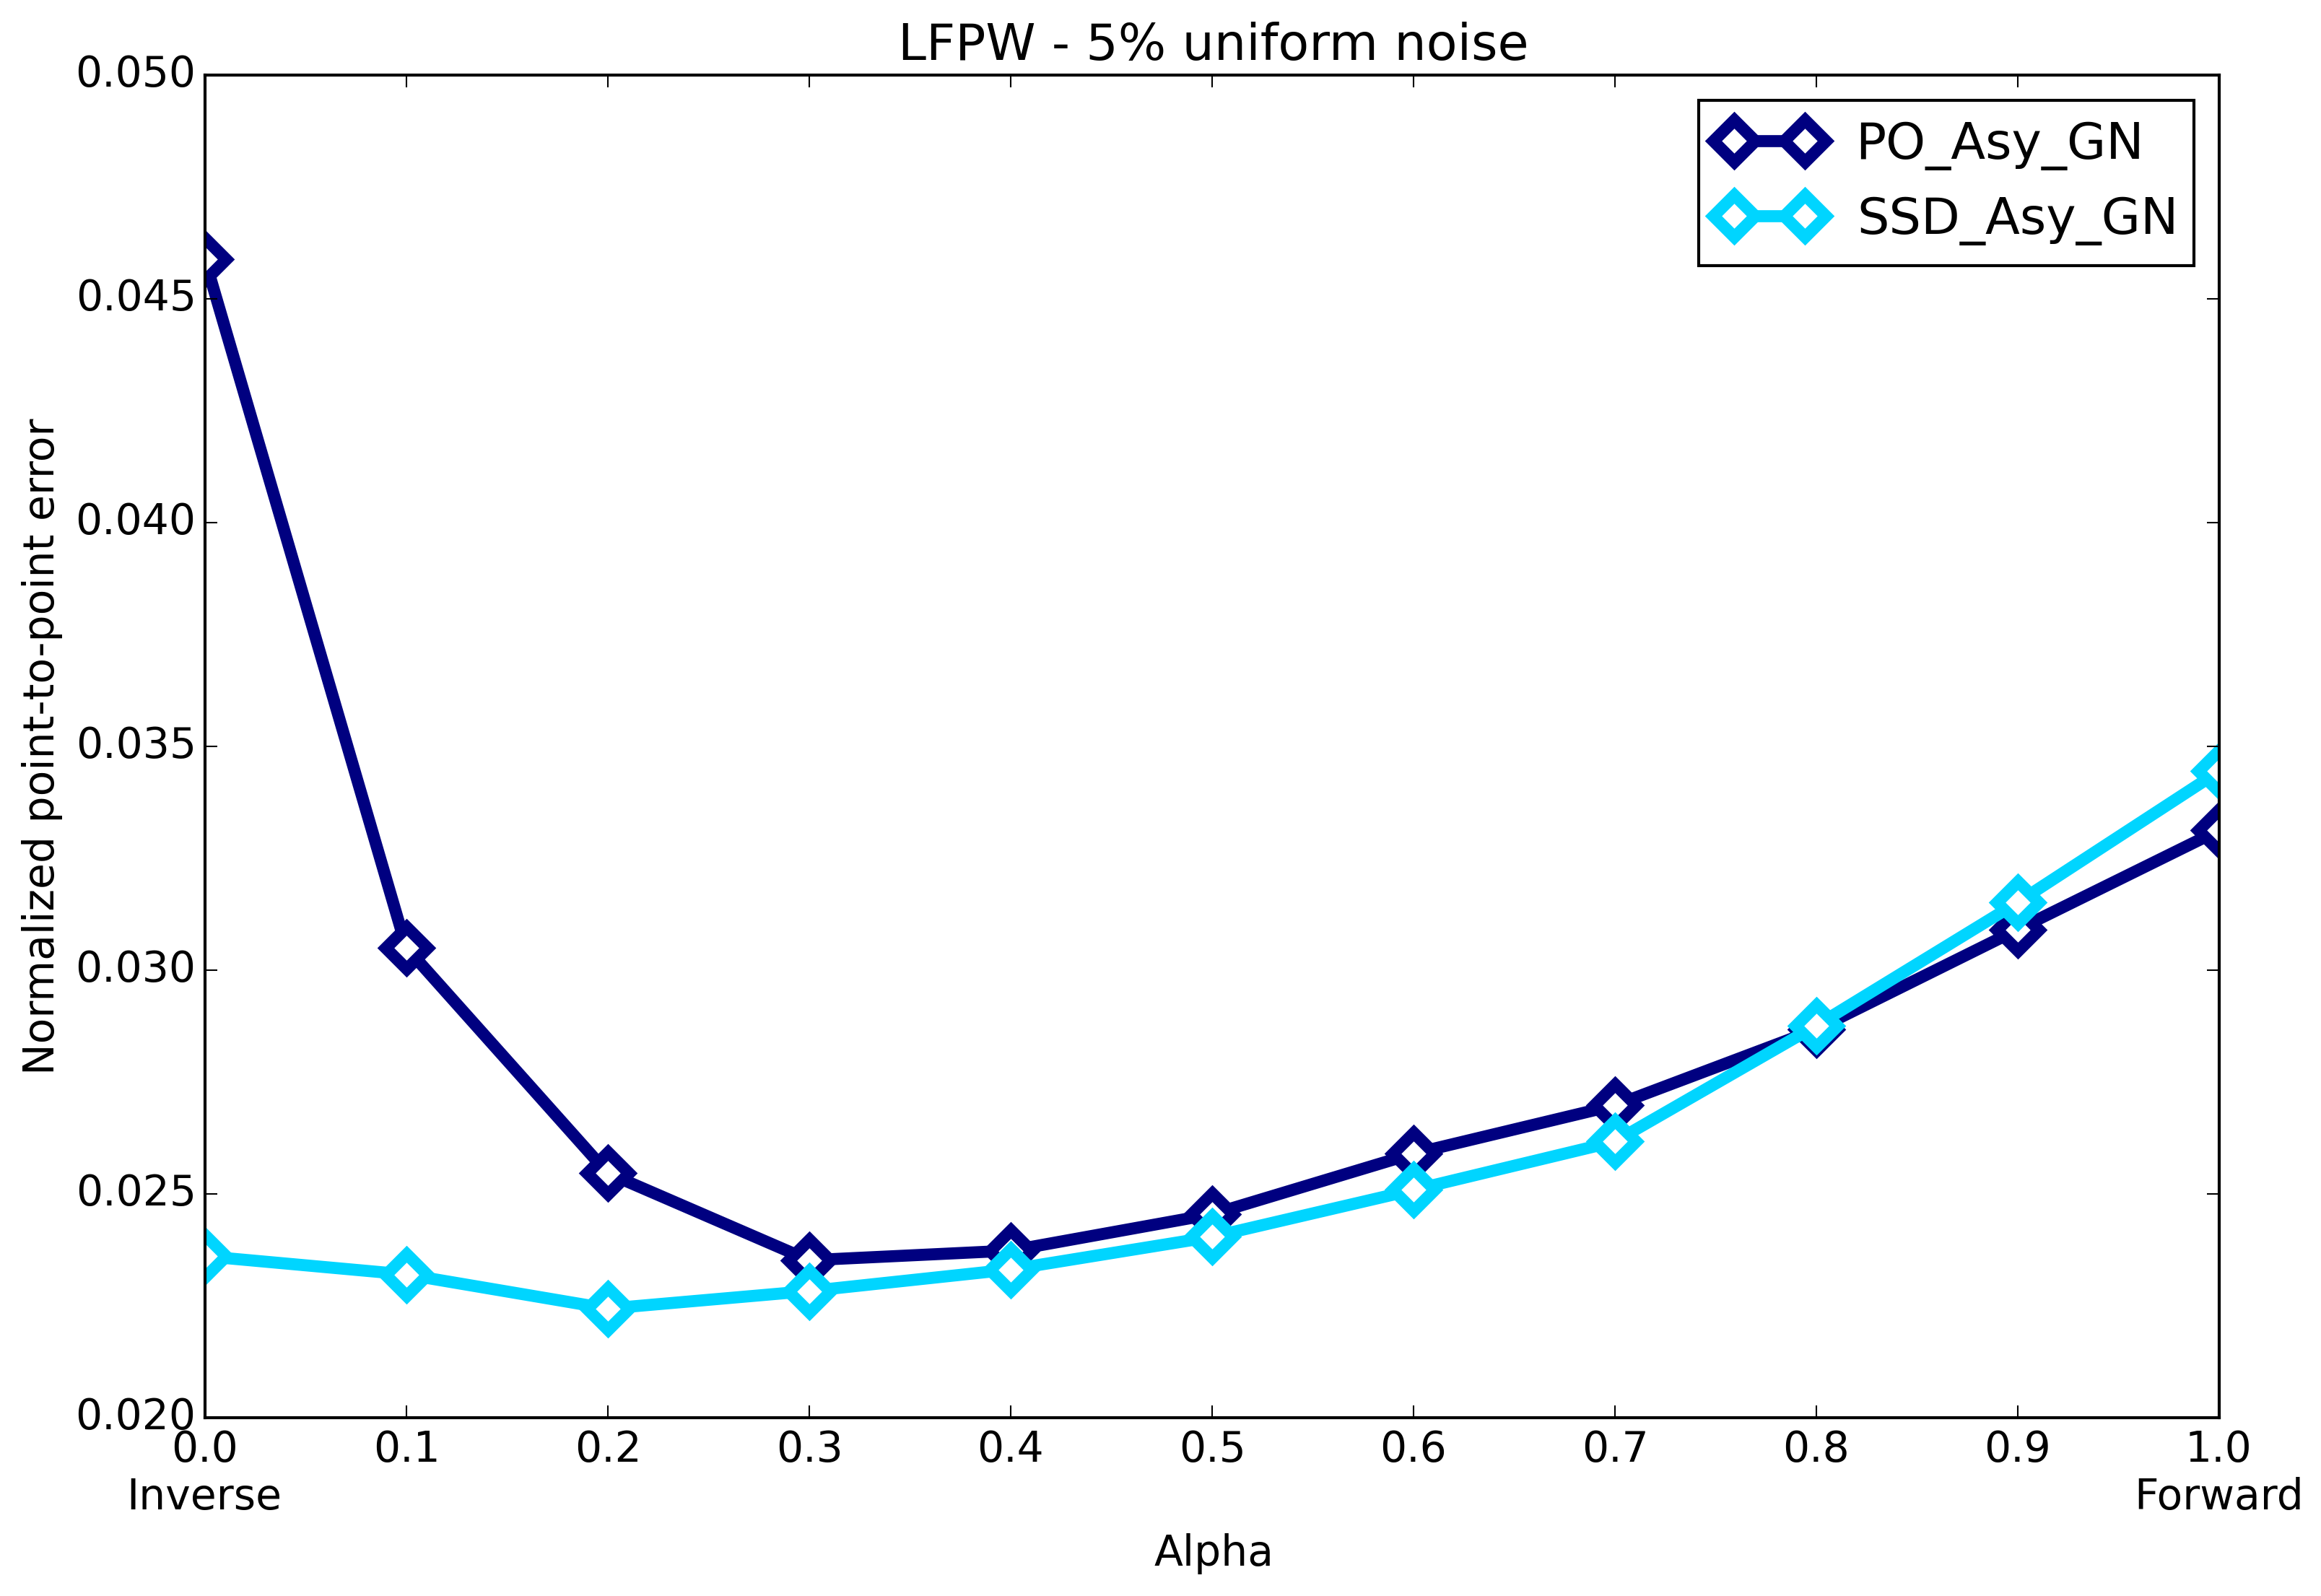
\includegraphics[width=0.48\textwidth]{experiments/alpha/mean_error_vs_alpha_5.png}
    \caption{Mean normalized point-to-point error vs alpha on the LFPW test dataset for all Asymmetric Gauss-Newton algorithms initialized with $5\%$ uniform noise.}
    \label{fig:ced_ssd_gn_5}
\end{figure}

\subsubsection{Sampling}

\begin{figure}[h!]
    \centering
    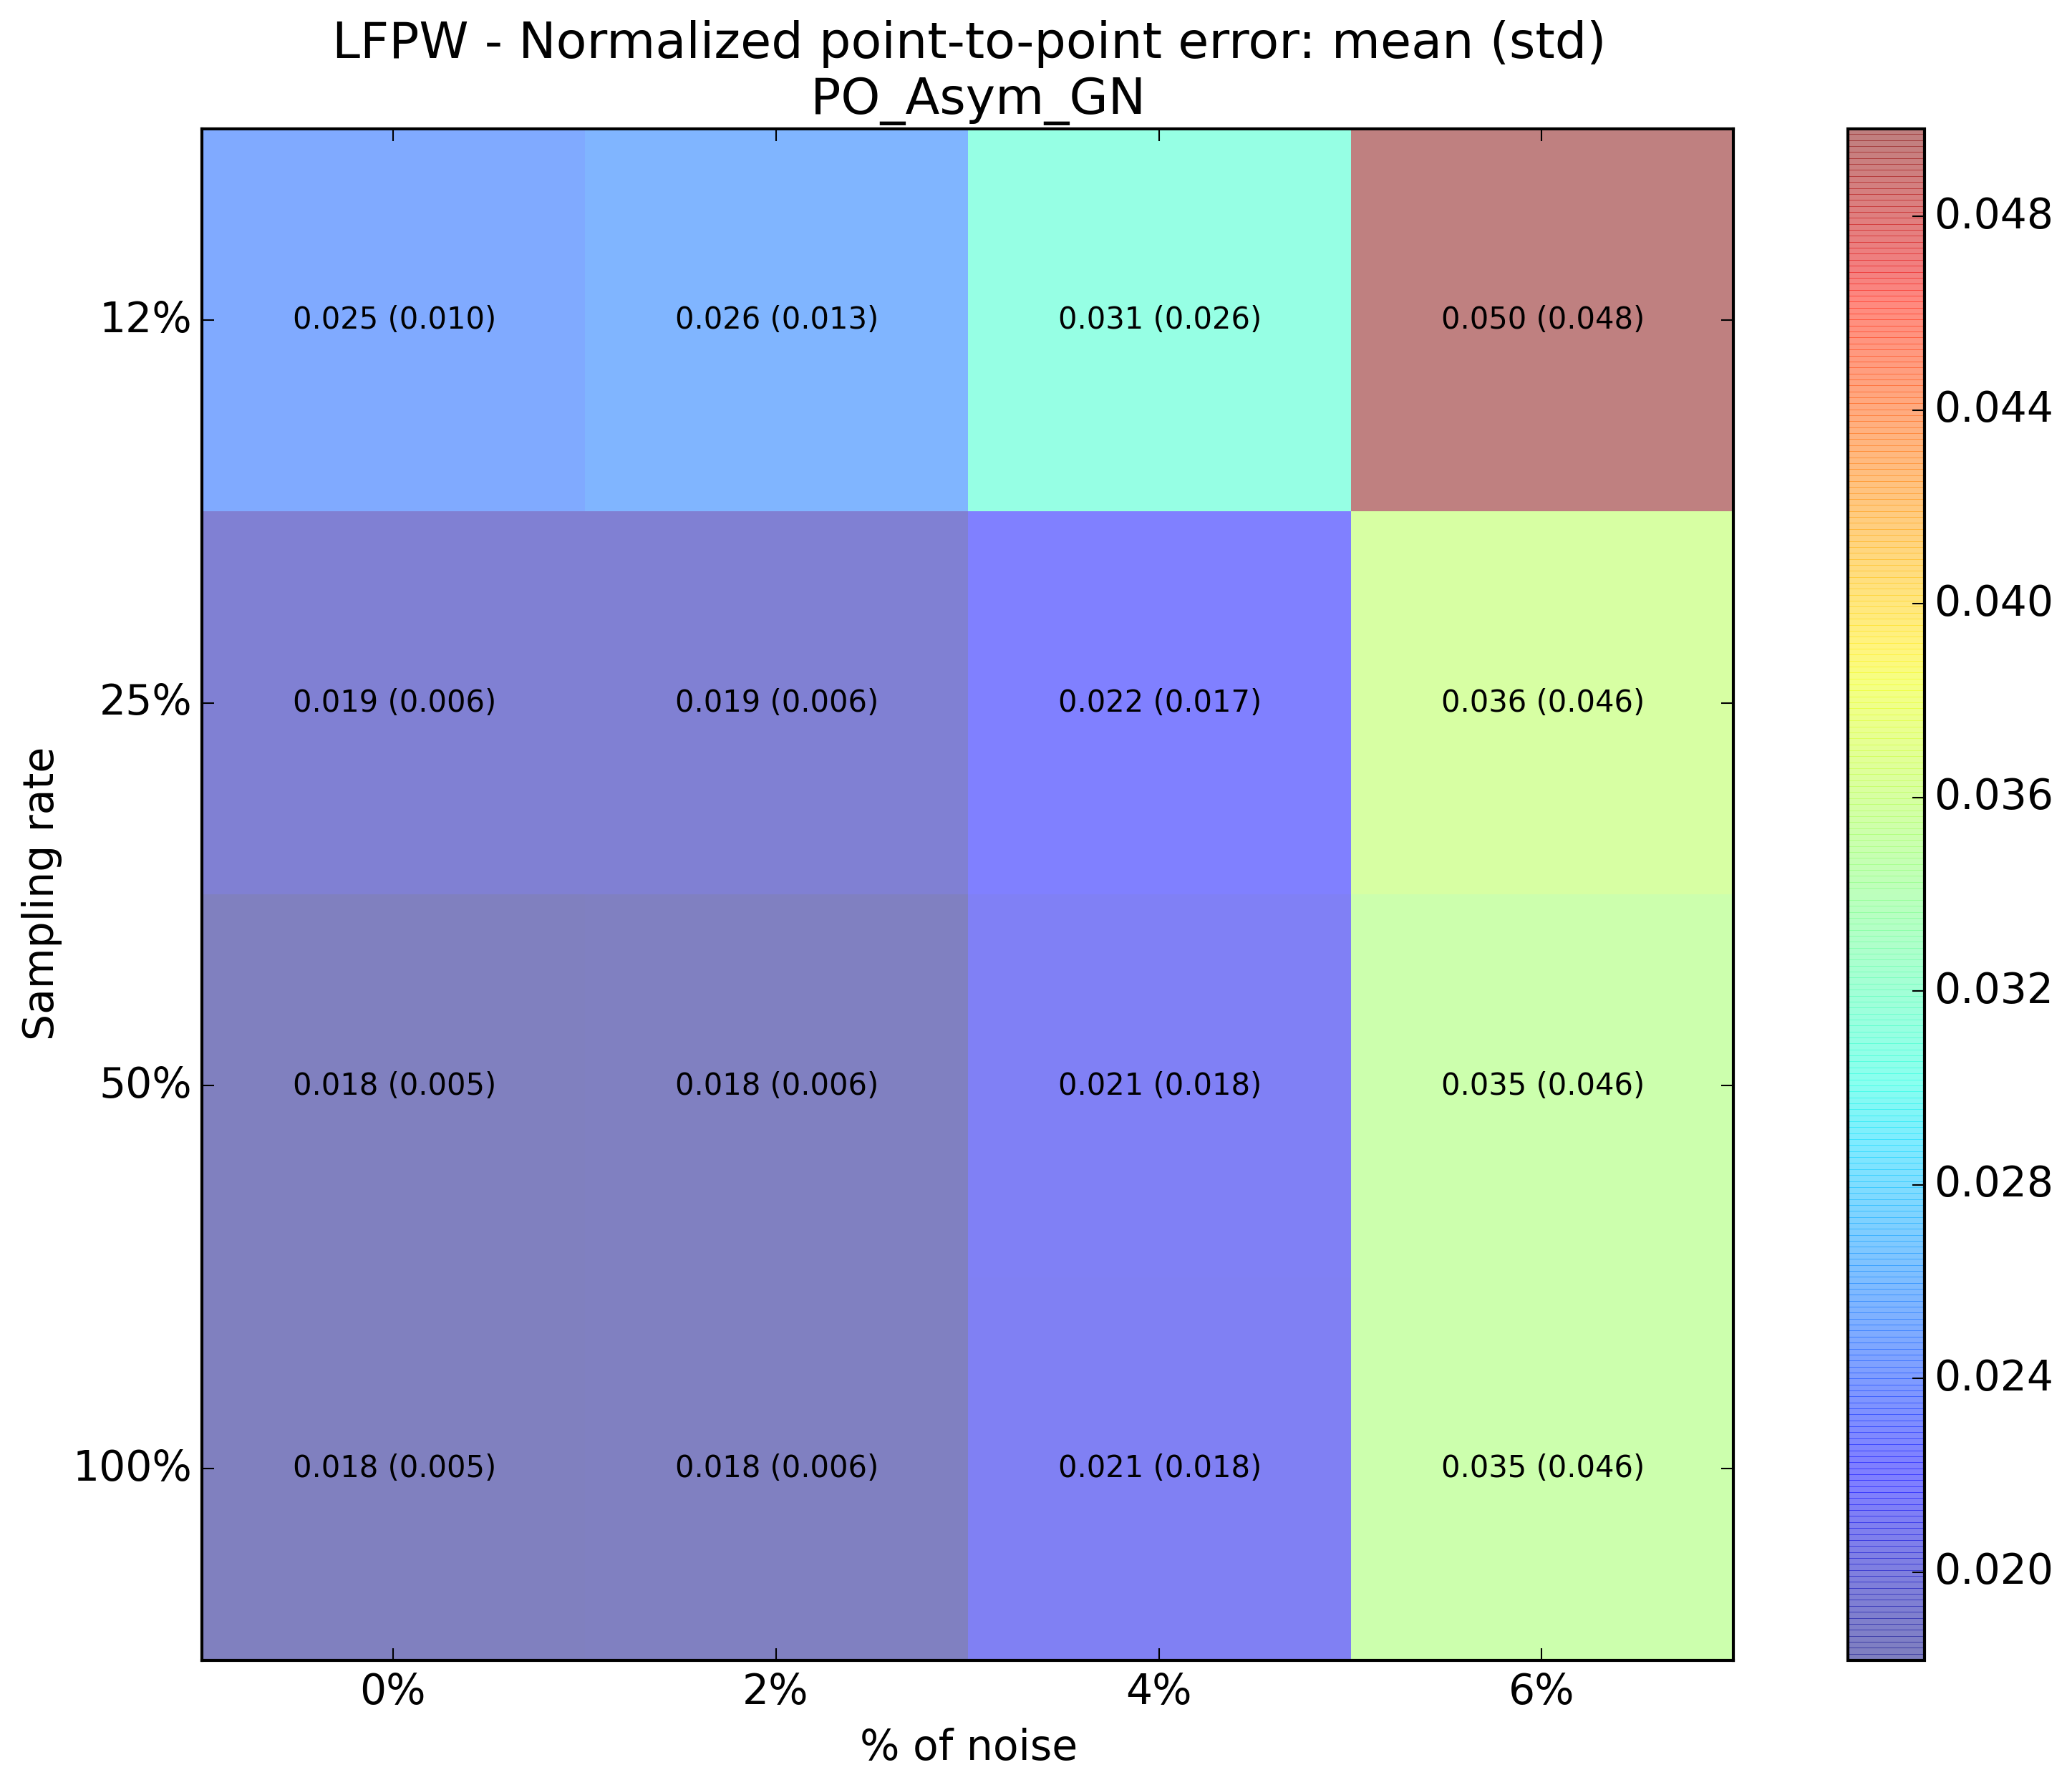
\includegraphics[width=0.45\textwidth]{experiments/sampling/po_asymmetric_gn/noise_vs_sampling_po_asymmetric.png}
    \caption{Mean and Std of normalized point-to-point error obtained on the LFPW test dataset by the Project-Out Asymmetric Gauss-Newton algorithm for different sampling rates versus different amounts of noise \% on the initialization.}
    \label{fig:noise_vs_sampling_po_asymmetric}
\end{figure}

\begin{figure}[h!]
    \centering
    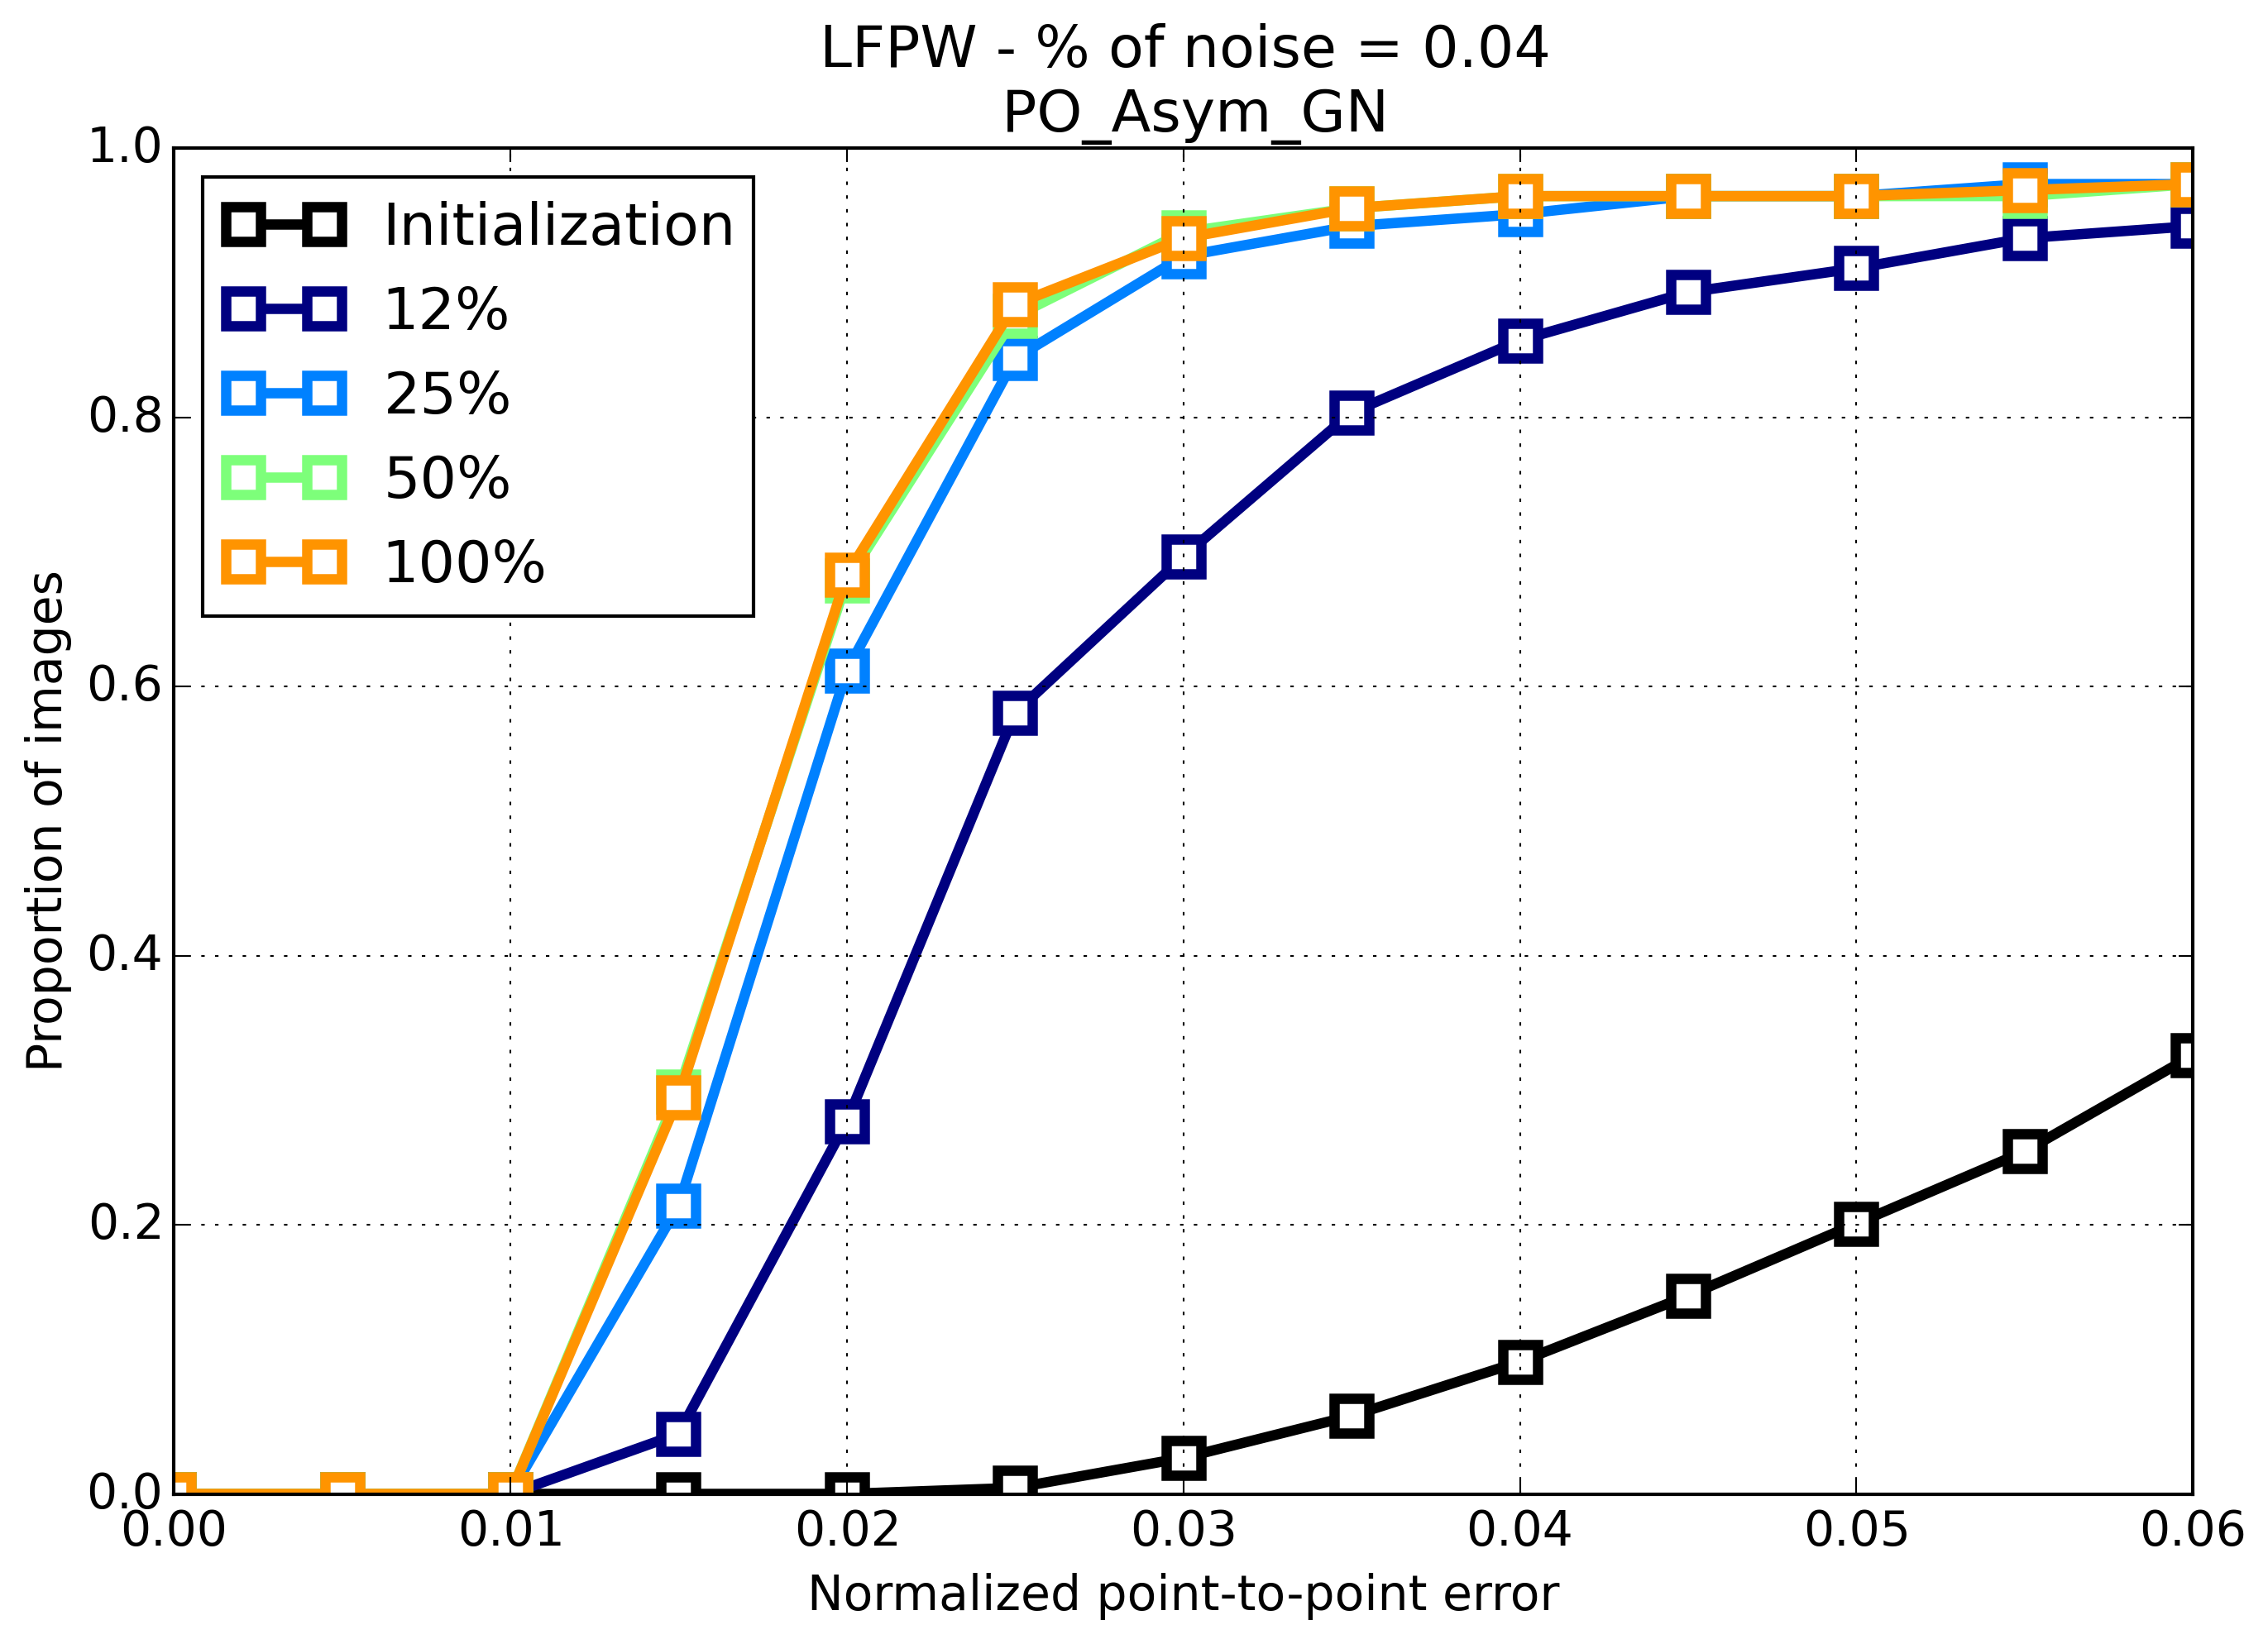
\includegraphics[width=0.50\textwidth]{experiments/sampling/po_asymmetric_gn/ced_po_asymmetric_gn_4.png}
    \caption{CED graph on the LFPW test dataset obtained by the Project-Out Asymmetric Gauss-Newton algorithm for $4$\% noise on the initialization.}
    \label{fig:ced_po_asymmetric_gn_4}
\end{figure}

\begin{figure}[h!]
    \centering
    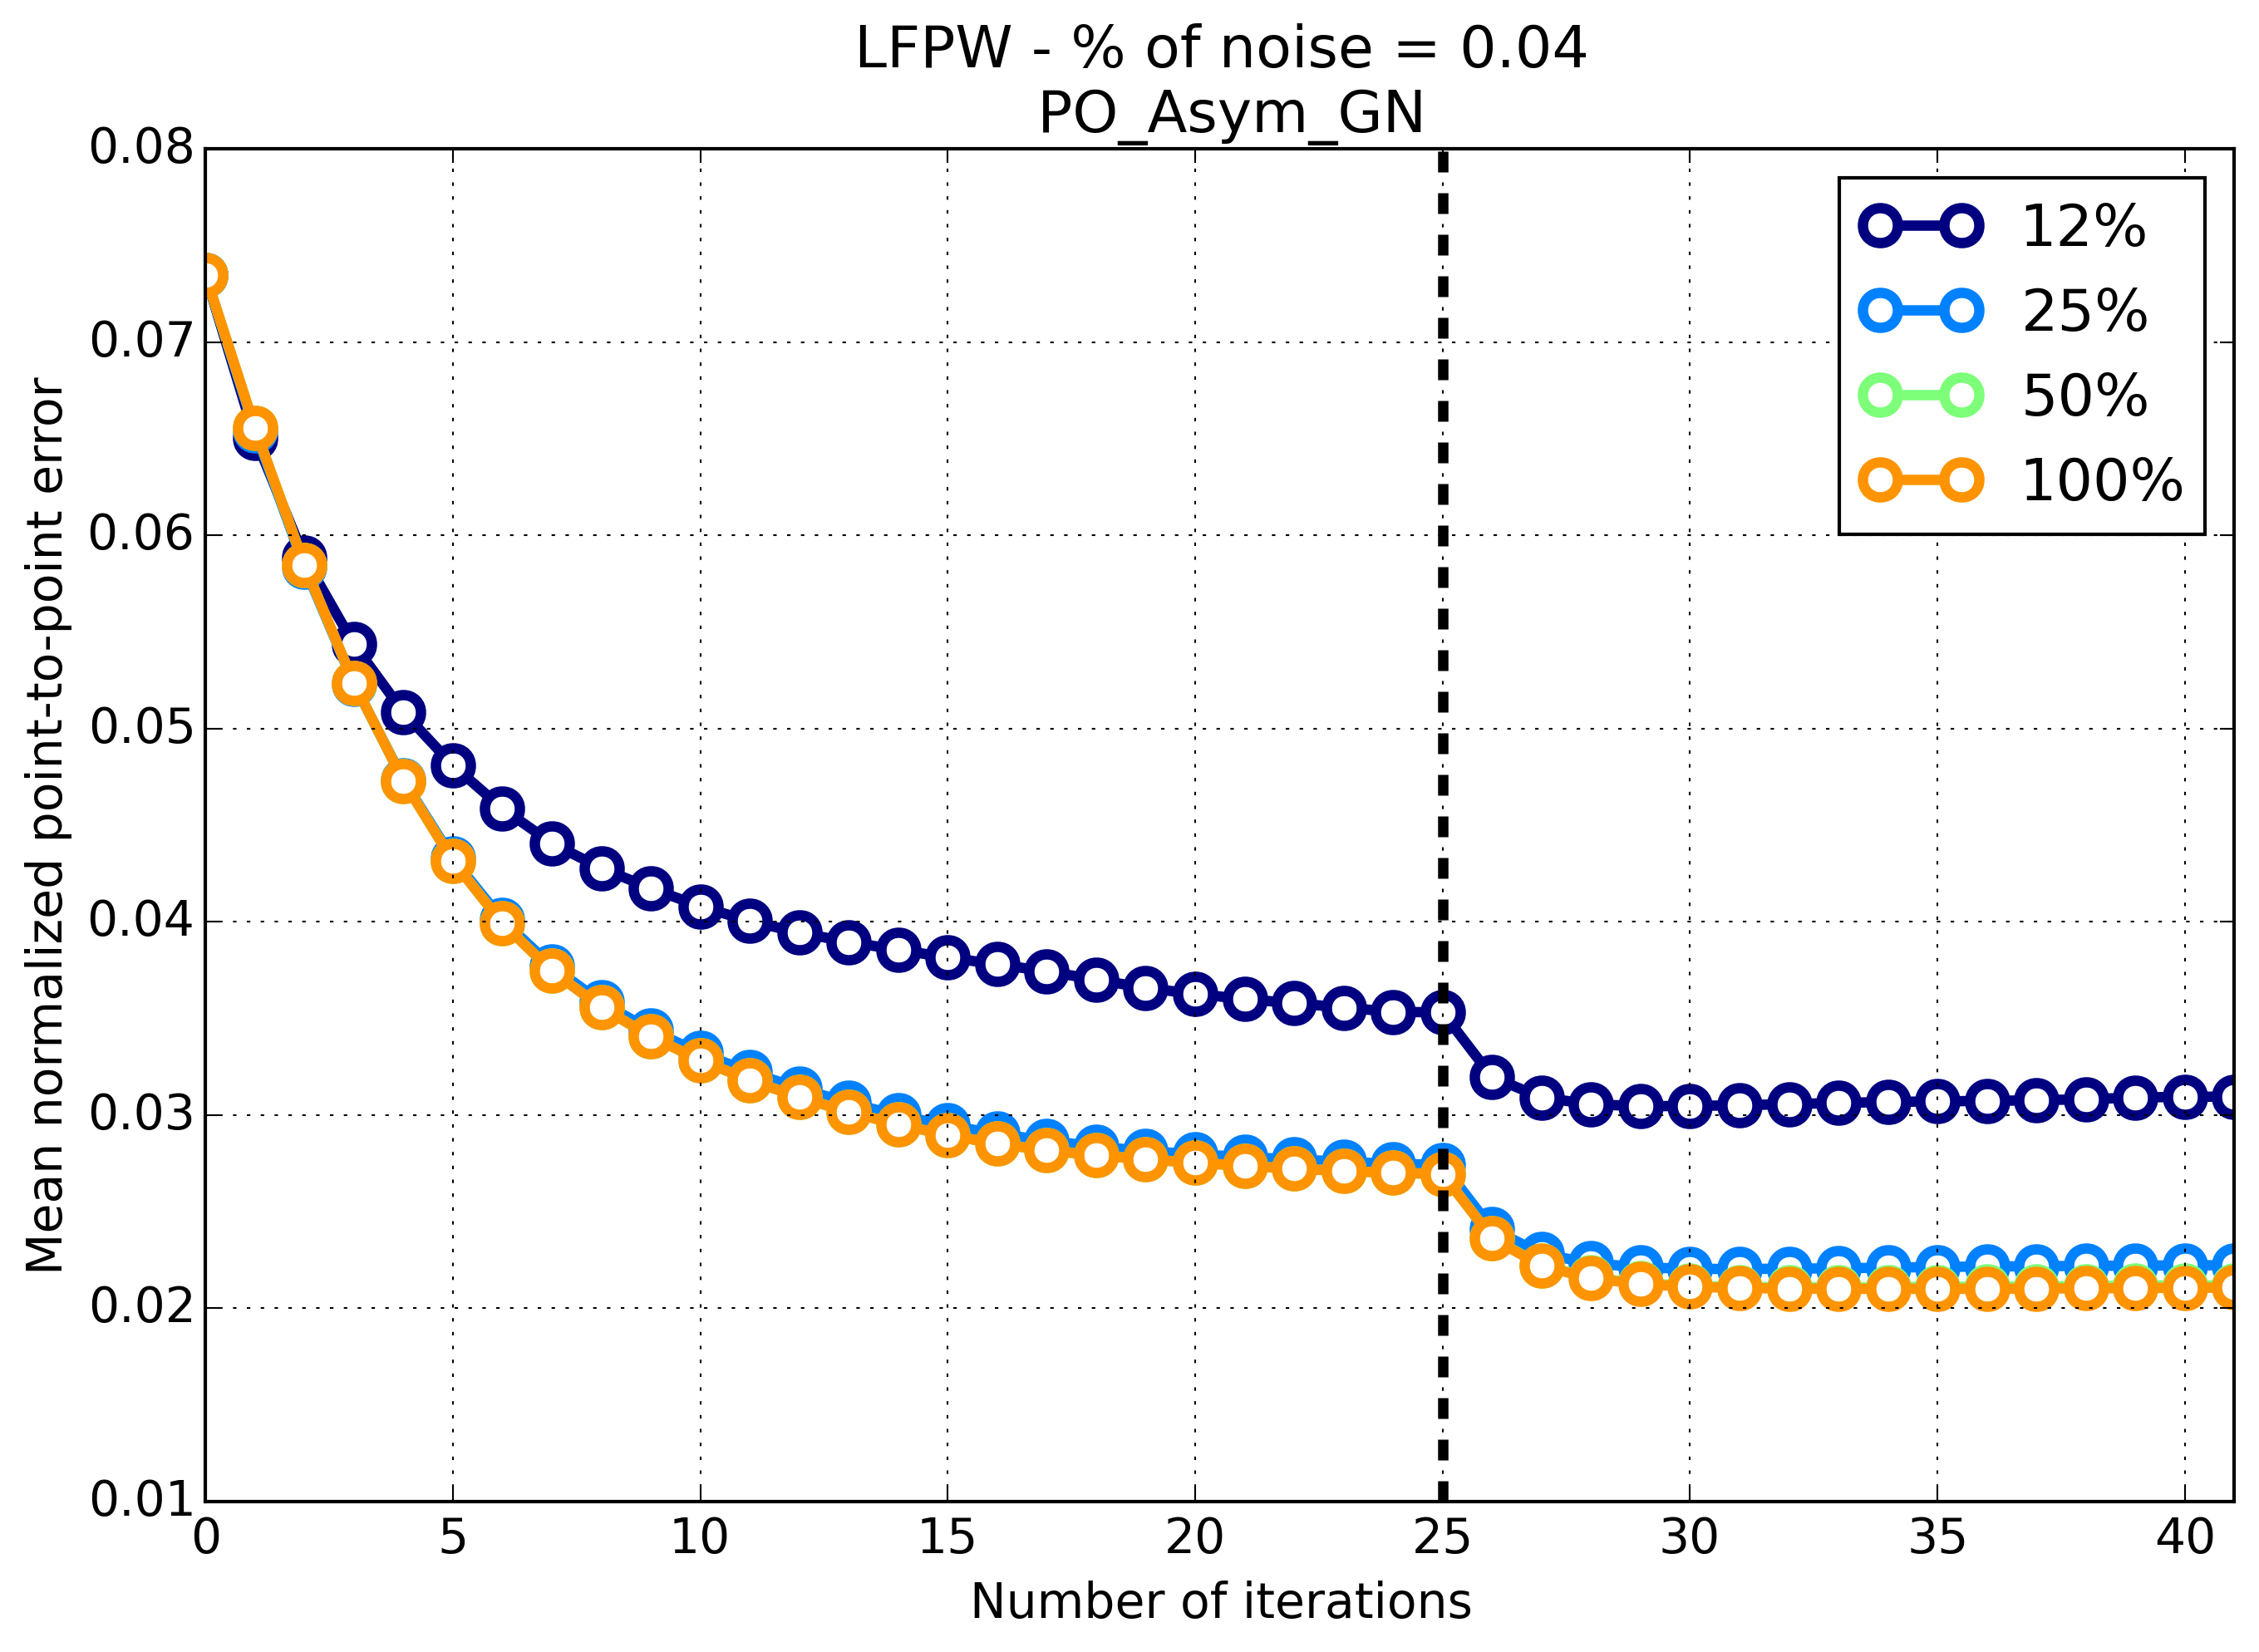
\includegraphics[width=0.50\textwidth]{experiments/sampling/po_asymmetric_gn/mean_error_vs_iters_po_asymmetric_gn_4.png}
    \caption{Mean normalized point-to-point error vs number of iterations graph on the LFPW test dataset obtained by the Project-Out Asymmetric Gauss-Newton algorithm for $4$\% noise on the initialization.}
    \label{fig:mean_error_vs_iters_po_asymmetric_gn_4}
\end{figure}

\begin{figure}[h!]
    \centering
    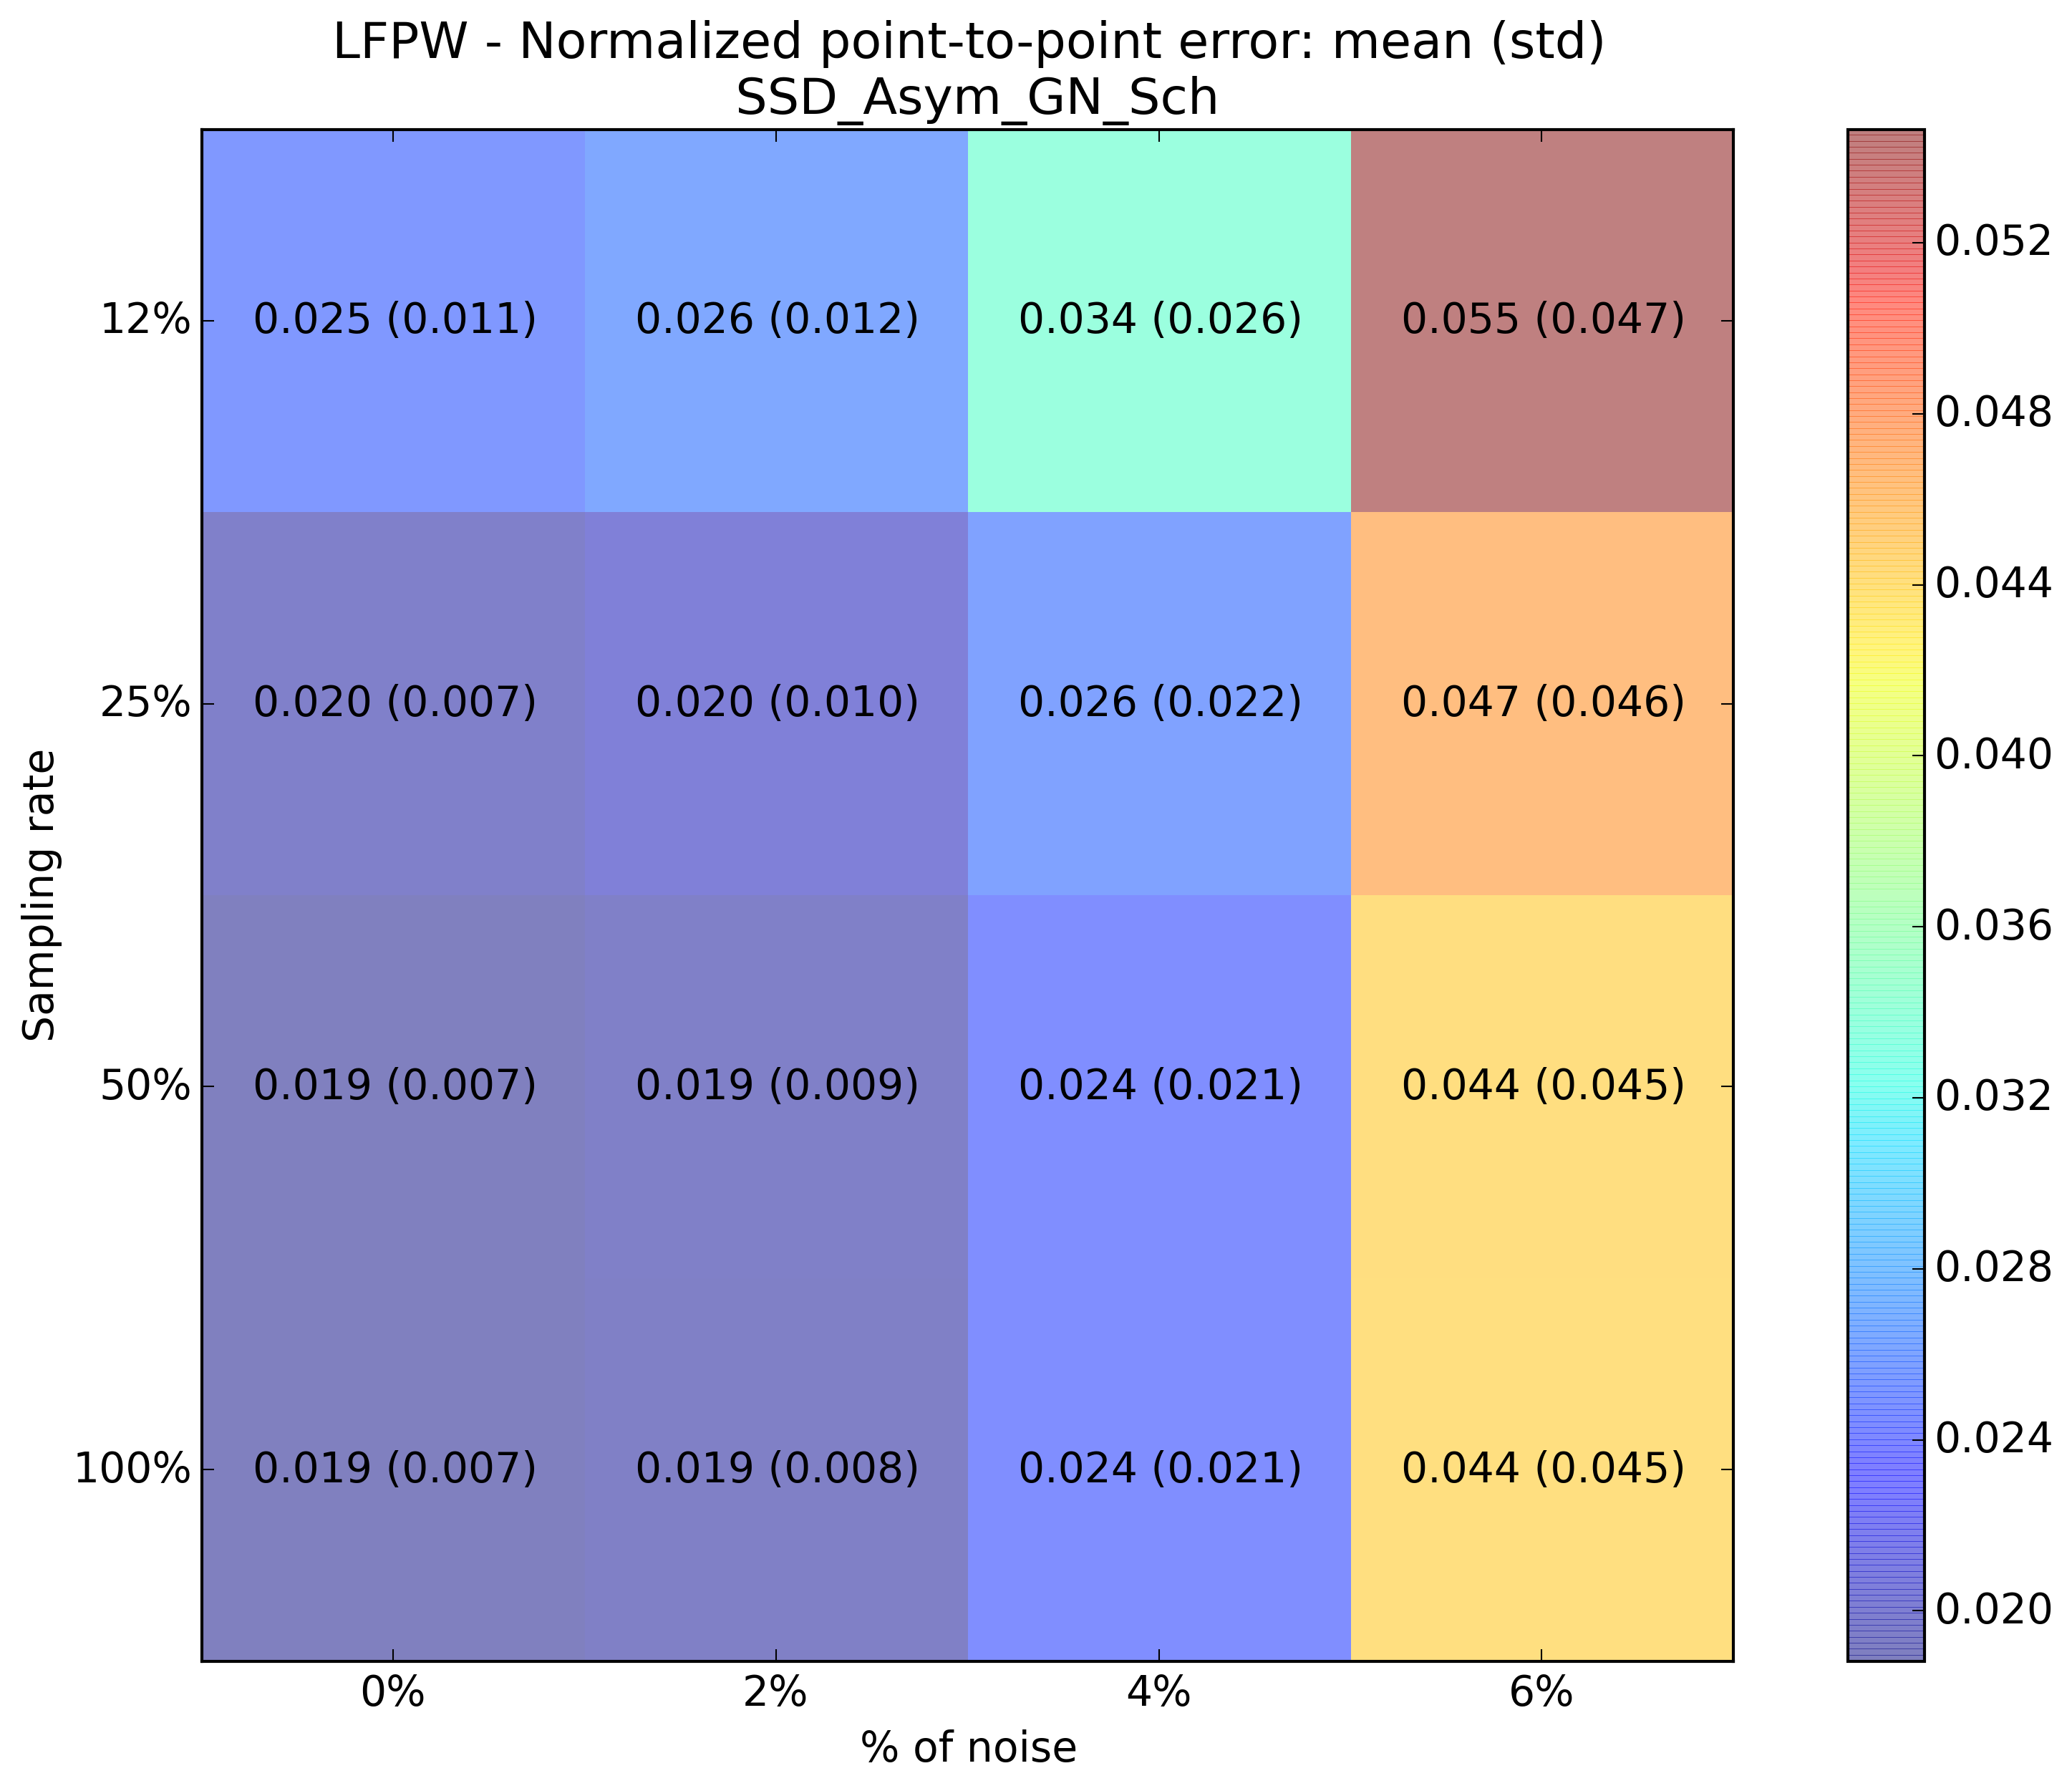
\includegraphics[width=0.45\textwidth]{experiments/sampling/ssd_asymmetric_gn/noise_vs_sampling_ssd_asymmetric.png}
    \caption{Mean and Std of normalized point-to-point error obtained on the LFPW test dataset by the SSD Asymmetric Gauss-Newton Schur algorithm for different sampling rates versus different amounts of noise \% on the initialization.}
    \label{fig:noise_vs_sampling_ssd_asymmetric}
\end{figure}

\begin{figure}[h!]
    \centering
    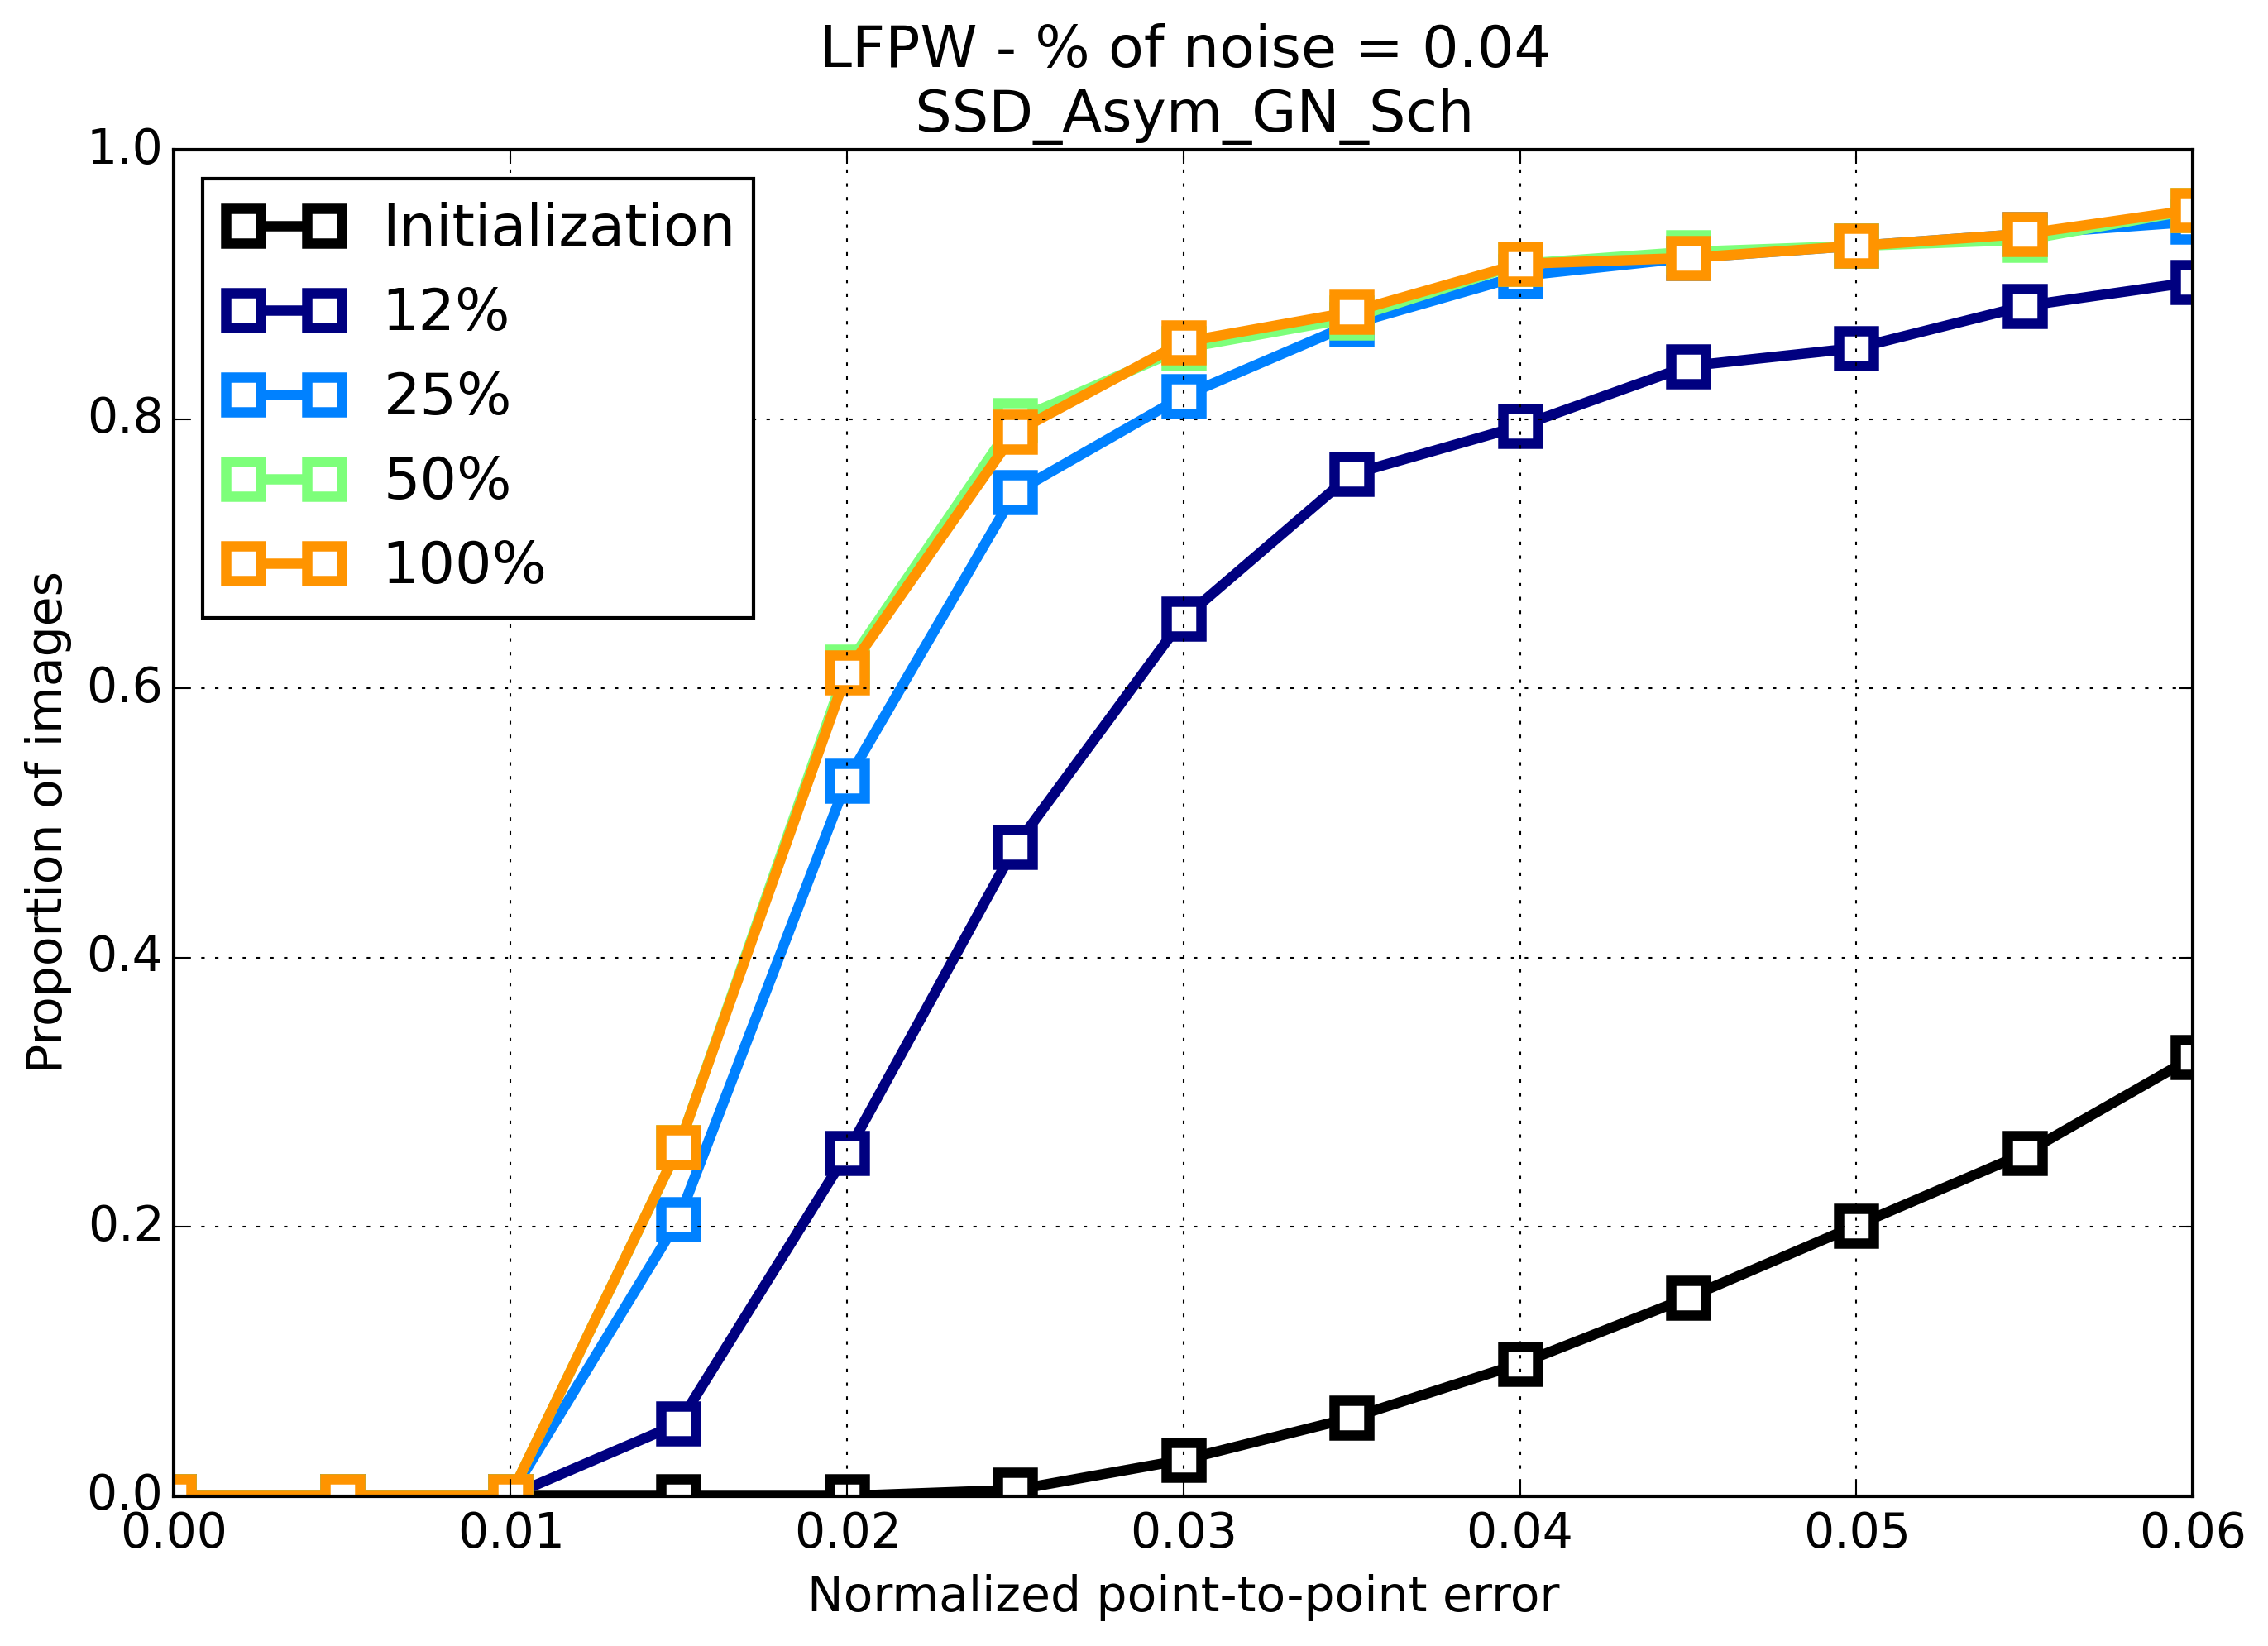
\includegraphics[width=0.50\textwidth]{experiments/sampling/ssd_asymmetric_gn/ced_ssd_asymmetric_gn_4.png}
    \caption{CED graph on the LFPW test dataset obtained by the SSD Asymmetric Gauss-Newton Schur algorithm for $4$\% noise on the initialization.}
    \label{fig:ced_ssd_asymmetric_gn_4}
\end{figure}

\begin{figure}[h!]
    \centering
    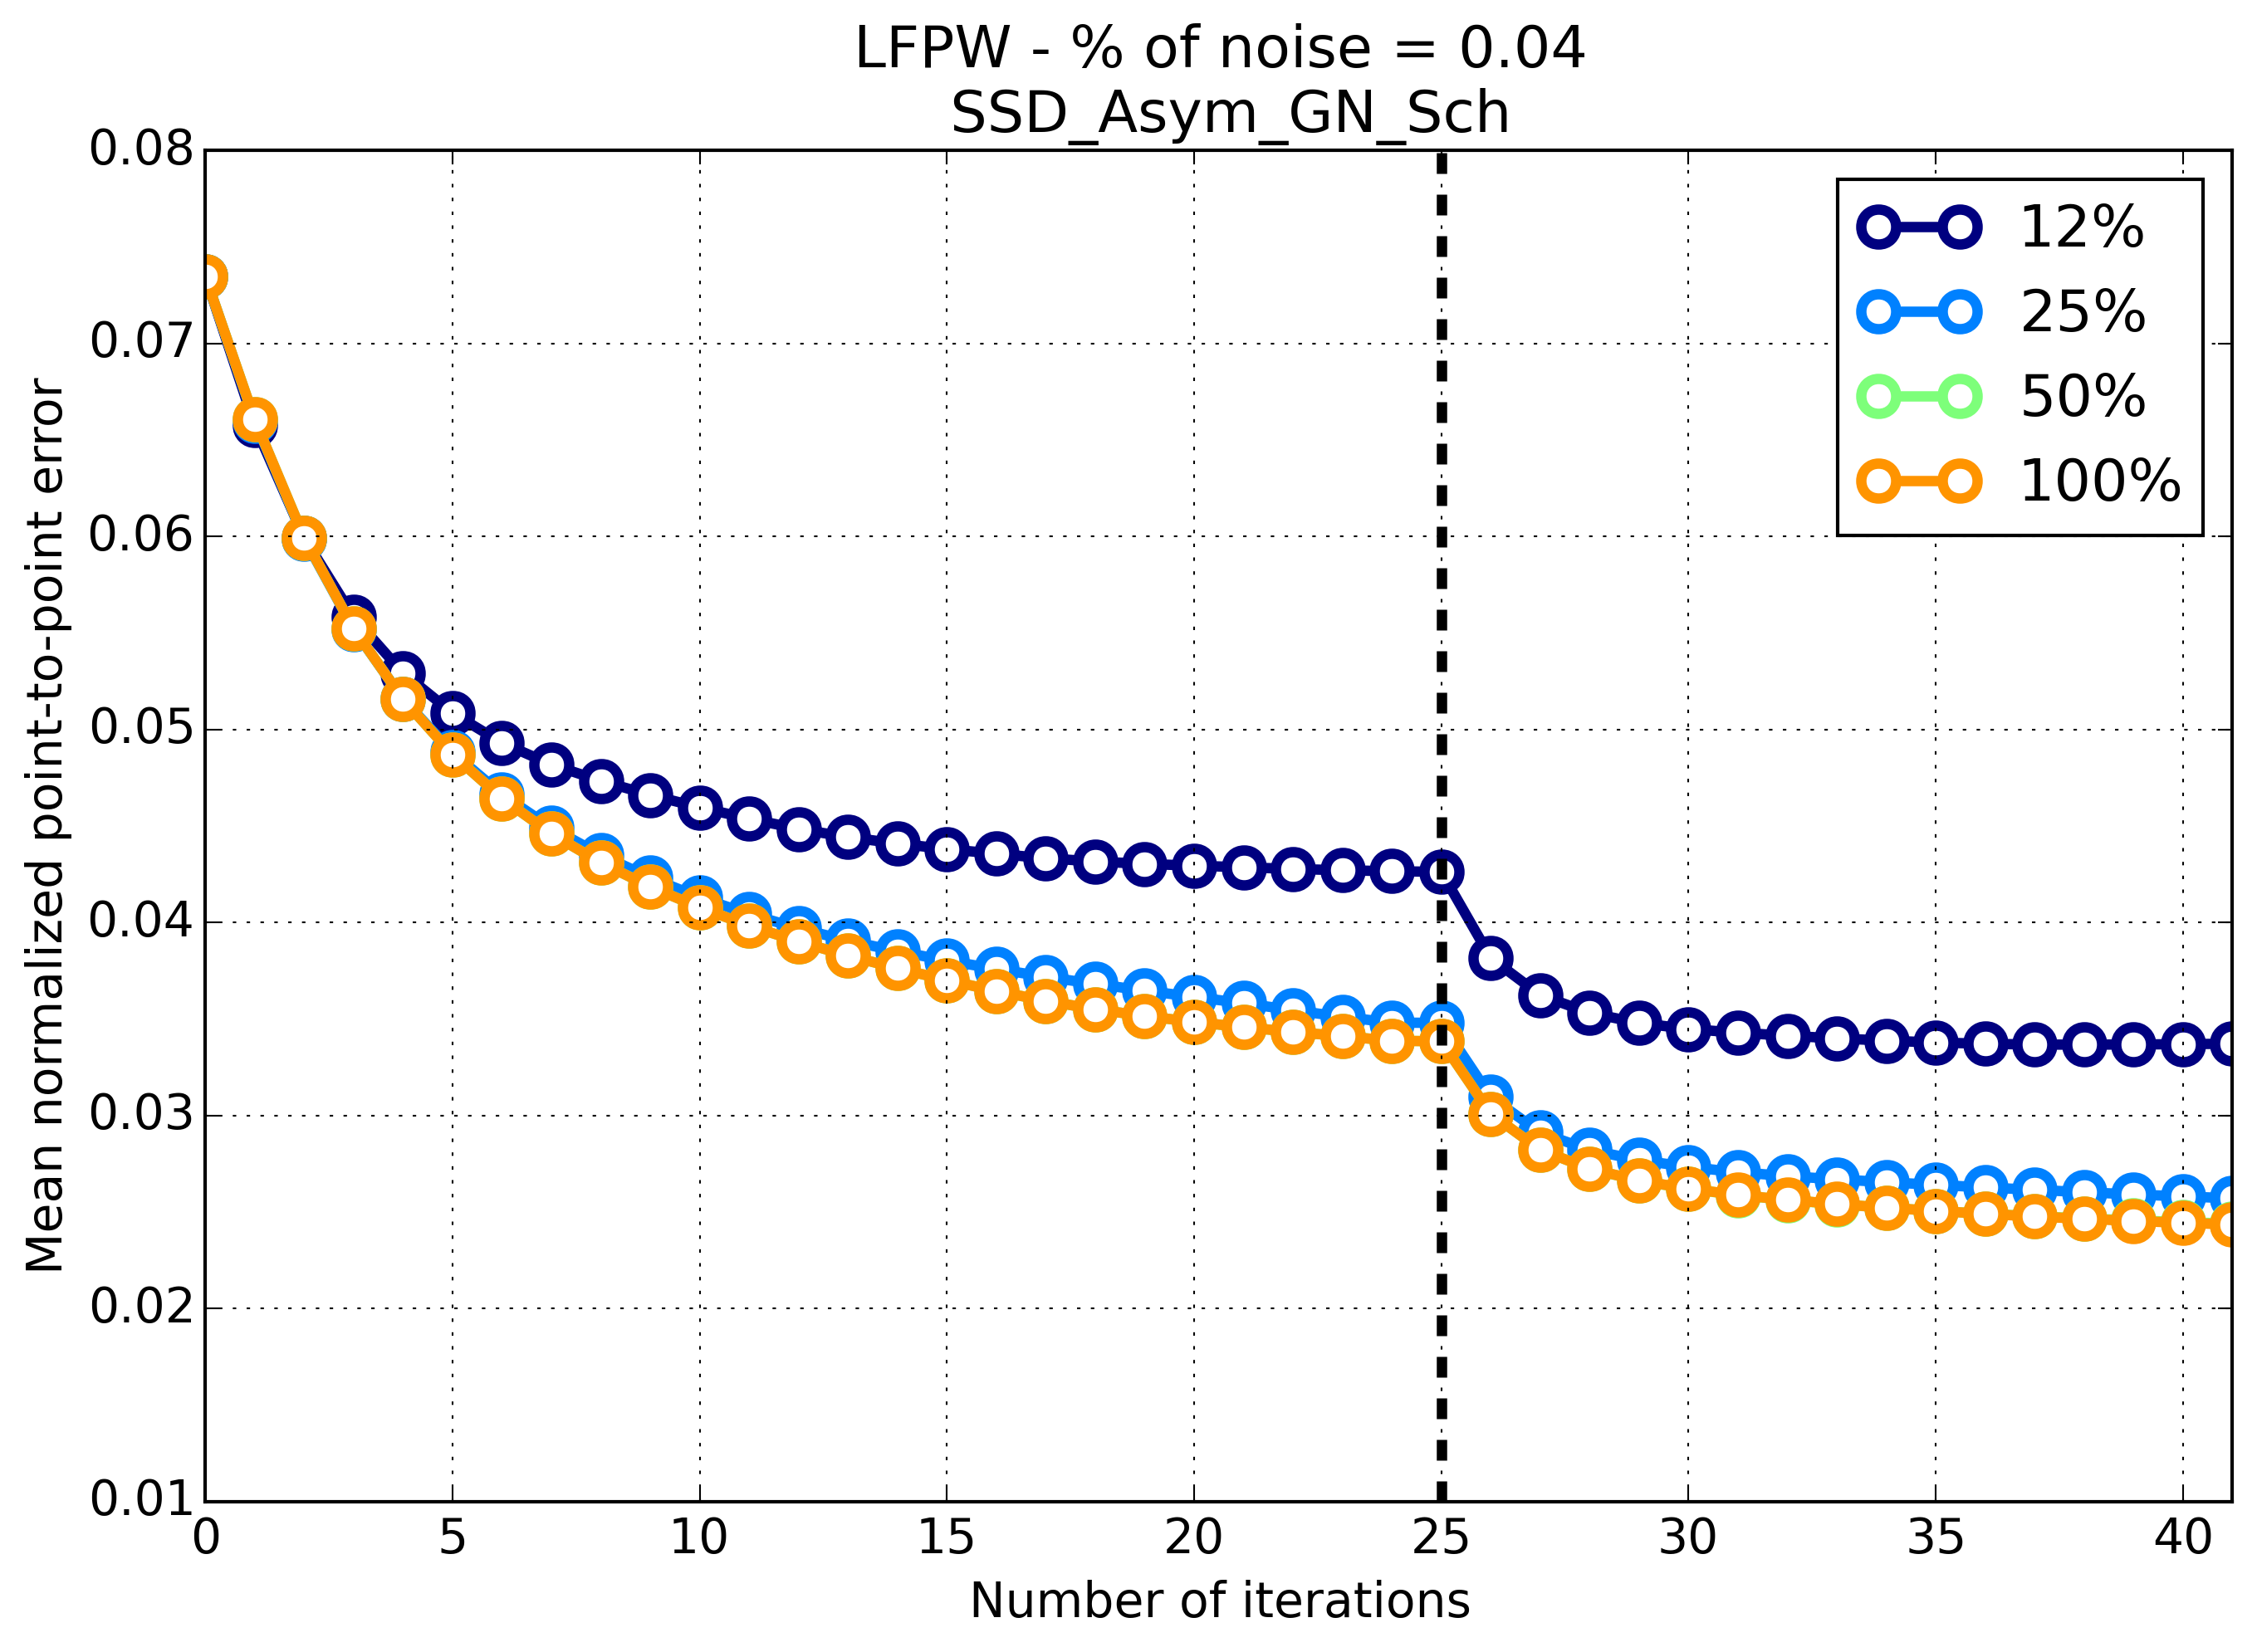
\includegraphics[width=0.50\textwidth]{experiments/sampling/ssd_asymmetric_gn/mean_error_vs_iters_ssd_asymmetric_gn_4.png}
    \caption{Mean normalized point-to-point error vs number of iterations graph on the LFPW test dataset obtained by the SSD Asymmetric Gauss-Newton Schur algorithm for $4$\% noise on the initialization.}
    \label{fig:mean_error_vs_iters_ssd_asymmetric_gn_4}
\end{figure}

\subsection{Comparison on Helen and AFW}





% This section reports the performance of the proposed method on the problem of face alignment in-the-wild. Results for two different experiments are reported. The first experiment compares the accuracy and convergence properties of the proposed Unified PIC-RLMS and AIC-RLMS algorithms with respect to those of PIC \cite{Baker2004}, AIC \cite{Papandreou2008} and and RLMS \cite{Saragih2011} on the popular LFPW \cite{Belhumeur2011} and Helen \cite{Le2012} datasets. The second experiment compares the performance of the previous algorithms against recently proposed state-of-the-art methods for face alignment in-the-wild, \ie the Supervised Descent Method of Xiong and De La Torre \cite{Xiong2013} and the Gauss-Newton Deformable Parts Model of Tzimiropoulos and Pantic \cite{Tzimiropoulos2014}, on the very challenging Annotated Faces in the Wild (AFW) dataset.

% \subsection{Comparison with AAMs and CLMs}
% Results for this experiment are reported over the 224 and 330 test images of the LFPW \cite{Belhumeur2011} and Helen\cite{Le2012} datasets. 66 points ground truth landmark annotations were provided by the iBUG group\footnote{\label{ibug_300}\url{http://ibug.doc.ic.ac.uk/resources/300-W/}}. All methods were initialized by perturbing the ground truth scale and translation parameters with Gaussian noise (rotations were not considered) and applying the resulting transformation to mean of the shape model. (Notice that this procedure produces initializations that are considerably more challenging than those reported in the recent AAM literature \cite{Tzimiropoulos2013, Tzimiropoulos2014}). The Cumulative Error Distributions (CED) for this experiment is shown in Figures \ref{fig:lfpw_exp1} and \ref{fig:helen_exp1}. Figures \ref{fig:lfpw_exp2} and \ref{fig:helen_exp2} shows the evolution of the mean normalized point-to-point error as a function of the number of iterations run by each algorithm. This experiment shows that our Unified AIC-RLMS approach considerably outperforms all other methods by a large margin on both datasets. More specifically, AIC-RLMS achieves a constant improvement of between 10\% to 20\% over PIC-RLMS and AIC at the significant region $0.020 < err > 0.040$ (at which the results are generally considered adequate by visual inspection). Note that the fast Unified PIC-RLMS algorithm is also the second most performant algorithm, surpassing both AIC and RLMS, on this particular experiment.

% \subsection{Comparison with state of the art}

% Results for this experiment are reported over the 337 images of the AFW \cite{Zhu2012} dataset. In this case, 49 points ground truth landmark annotations for this dataset were again provided by the iBUG group\footnoteref{ibug_300}. Results for \cite{Xiong2013} and \cite{Tzimiropoulos2014} were directly obtained using the publicly available models and fitting code kindly provided by the authors\footnote{\url{http://www.humansensing.cs.cmu.edu/intraface/}}$^{,}$\footnote{\url{http://ibug.doc.ic.ac.uk/resources/gauss-newton-deformable-part-models-face-alignment/}}. Note that, the provided models have been potentially trained using thousands of images in contrast to the only 813 images used to trained our method. In this experiment, all algorithms were initialized using the bounding box provided by our own in-house implementation of the face detector of \cite{Zhu2012}. The CED for this experiment are reported in Figure \ref{fig:afw_exp}. The results show that our Unified AIC-RLMS algorithm achieves state-of-the-art results on the AFW dataset, considerably outperforming both the Gauss-Newton Deformable Parts-Model of Tzimiropoulos and Pantic \cite{Tzimiropoulos2014} (which can be extremely accurate but sensitive to inaccurate initializations) and the SDM method of Xiong and De la Torre \cite{Xiong2013} (which can deal with very noisy initializations but is significantly less accurate than our method).

% \begin{figure}[t!]
% \centering
% \includegraphics[width=0.38\textwidth]{figures/graph7.png}
% \caption{Cumulative Error Distributions over 49 landmarks for the AFW dataset.}
% \label{fig:afw_exp}
% \end{figure}
